\chapter{Proofs and Supplementary Details for Chapter~\ref{ch:latent-bandits}}
\label{app:latent-bandits}

\aigen{This appendix provides the supporting lemmas, the proof of the de Finetti theorem for stateless and transition-agnostic contextual decision processes, the proofs of the offline subspace estimation guarantee (Theorem~\ref{thm:delta-off}), the online regret upper bounds for Algorithms~\ref{alg:local-ucb} and \ref{alg:proball-ucb} (Theorems~\ref{thm:local-ucb} and \ref{thm:proball-ucb}), the hybrid minimax lower bound, additional algorithmic variants (pseudoinverse subspace estimation and projected confidence-ball Thompson sampling), and supplementary experimental ablations for Chapter~\ref{ch:latent-bandits}.}


% --- From additional-lemmas.tex ---
\section{Additional Lemmas and Discussion}\label{app:additional-lemmas}

\subsection{Broader Impacts}\label{subapp:broader-impacts}
Often, protected groups with private identities have temporal behavior correlated with their private identities. Latent state estimation methods have the potential to identify such private identities online, and must be used with care. Use of such methods should comply with the relevant privacy and data protection acts, and corporations with access to a large customer base as well as governments should be mindful of the impact of the use of latent state methods on their customers and citizens respectively.

\subsection{Coherence with Equality is Necessary}
\begin{restatable}[Coherence with Equality is Necessary]{lemma}{CoherenceEquality}\label{lem:coh-equality}
    There exists a stateless decision process that is exchangeable and not coherent but satisfies the following property: for any two action sequences $\tau, \tau'$ of lengths $H$ and $H'$ sharing the same actions $(a_h, \dots a_k)$ from index $h$ to $k$, with $\gF_{H}(\tau) = (Y_1, \dots Y_{H})$ and $\gF_{H'}(\tau') = (Y_1', \dots Y_{H'}')$, we have $(Y_h, \dots Y_k) \sim (Y_h', \dots Y_k')$. Additionally, since the SDP is not coherent, it is not a latent bandit.
\end{restatable}

\begin{proof}
    Consider an SDP with action set $\gA = \{0,1\}$ equipped with a random variable $\theta \in \{0, 1\}$ distributed as $Ber(1/2)$. If the first action is $0$, then all rewards are given by $\theta$. If the first action is $1$, then the first reward $X_1 = \theta$ while all future rewards are $1-\theta$.

    Notice now that for any timestep $h$, its rewards are $Ber(1/2)$. We note that this process is clearly exchangeable. Moreover, this process is coherent in a weaker sense -- for any two action sequences $\tau, \tau'$ of lengths $H$ and $H'$ sharing the same actions $(a_h, \dots a_k)$ from index $h$ to $k$, with $\gF_{H}(\tau) = (Y_1, \dots Y_{H})$ and $\gF_{H'}(\tau') = (Y_1', \dots Y_{H'}')$, we have $(Y_h, \dots Y_k) \sim (Y_h', \dots Y_k')$. That is, the reward subsequences are only equal \textit{in distribution}. This is easy to see, since if $a_1$ is not included in the action subsequence or if $a_1 = 0$, the reward subsequence is always given by $(X, \dots X)$ for $X \sim Ber(1/2)$. If $a_1 = 1$ and $a_1$ is in the action subsequence, then the reward subsequence is always given by $(-X, X,  \dots X)$ for $X \sim Ber(1/2)$.

    However, the reward subsequences are not equal \textit{in value}. If the action subsequence is inside two action sequences $\tau = (a_1, \dots a_H)$ and $\tau' = (a'_1, \dots a'_H)$ with $a_1 = 0$ and $a_1'=1$, then their rewards are negatives of each other. So, this SDP is not coherent. This means that this SDP is not a latent bandit.
\end{proof}

\subsection{Contexts, Latent State and Behavior Policy cannot be Dependent}
\NecStochUnconf*

\begin{proof}

Let $e_1, e_2$ be the standard basis of $\R^2$. For all these examples, our two latent bandits will satisfy the following:
\begin{itemize}
        \item \textbf{Latent contextual bandit $1$:} Let $\btheta$ take values $e_1+e_2$ and $-e_1-e_2$ with probability $1/2$ each.
        \item \textbf{Latent contextual bandit $2$:} Let $\btheta$ take values $e_1-e_2$ and $e_2-e_1$ with probability $1/2$ each.
    \end{itemize} 
    

\subsubsection{Contexts cannot be dependent on each other}
We consider two actions, so $\gA = \{0,1\}$
    We have two contexts $x, y$ so that $\phi(x,0) = e_1$, $\phi(x,1) = 2e_1$ while $\phi(y,0) = e_2$, $\phi(y,1) = 2e_2$. We design them to be dependent so that any trajectory either only sees $x$ or only sees $y$. However, $x$ and $y$ are both seen with probability $1/2$. Pick $\pi_b$ so that it takes each action with probability $1/2$. Now note that the mean reward of $x, 0$ in either latent bandit takes values $\pm 1$ with probability $1/2$. So, the offline data distributions are also indistinguishable and every context-action pair is seen with probability at least $1/4$.
\subsubsection{Contexts and latent state cannot be dependent}
We consider two actions, so $\gA = \{0,1\}$
Again, consider two contexts $x, y$ so that $\phi(x,0) = e_1$, $\phi(x,1) = 2e_1$ while $\phi(y,0) = e_2$, $\phi(y,1) = 2e_2$. Let us say that for either latent bandit and for any $\btheta$, the context distribution is a Dirac-$\delta$ over the context whose features have a positive dot product with $\btheta$. Then, note that either context is seen in both latent bandits with probability $1/2$. Again, let $\pi_b$ take either action with probability $1/2$. So, the offline data distributions are indistinguishable and every context-action pair is seen with probability at least $1/4$.
\subsubsection{Latent state and behavior policy cannot be dependent}
We consider four actions, so that $\gA = \{0,1,2,3\}$. Let there be a single context $x$ with $\phi(x,0) = e_1, \phi(x,1) = e_2, \phi(x,2) = -e_1, \phi(x,3) = -e_2$. For any latent state $\btheta$ in either bandit, let $\pi_b$ be uniform over the actions that have a positive dot product with $\btheta$. It is then easy to see that the offline data distributions are indistinguishable and every context-action pair is seen with probability at least $1/4$.
\end{proof}


% --- From de-finetti.tex ---
\section{A de Finetti Theorem for decision processes}

\subsection{Discussion on \cite{liu2023definition}'s smaller class of generalized bandits}\label{subapp:de-finetti-disc}
We prove the de Finetti theorem for a very general formulation of decision processes. However, past work \citep{liu2023definition} has studied a simpler generalization of bandits, namely a stochastic process valued in $\R^{\gA}$. A sample point in this space is a \textit{sequence of functions} in $\gA \to \R$, which rules out the possibility of adaptivity. In contrast, a sample point in our space is a \textit{function of sequences}, which subsumes all sample points of their space, but allows for adaptivity. 

\cite{liu2023definition} are able to use the original de Finetti theorem on their random process directly, but work with a much more restrictive kind of decision process. We show that even when considering much more general stateless decision processes, latent bandits are the "right" objects produced by a de Finetti theorem for stateless decision processes.

\subsection{Proof of the De Finetti Theorem for Stateless Decision Processes}
\label{app:definetti}

\paragraph{A note on $F$, measurability and well-definedness in the definition of a latent bandit.} Recall that $F$ in the definition of a latent bandit needs to be a measurable map $\Omega \to (\gA \to \gP(\Real))$. To define measurability for the output space of functions $(\gA \to \gP(\Real))$, we endow $\gP(\Real)$ with the topology of weak convergence, endow the space $\gP(\Real)^\gA$ of maps $\gA \to \gP(\Real)$ with the topology of point-wise convergence, and require $F$ to be measurable w.r.t. the induced Borel $\sigma$-algebra. We also recall two abuses of notation in the definition of a latent bandit. First, we abuse notation to define the random measure $F(a) := (\omega \mapsto F(\omega)(a))$. Second, we also abuse notation to conflate $F(a)$ with the curried map $\kappa_a(\omega, B) := F(a)(\omega)(B)$, which is a map $\Omega \times \gB \to [0,1]$. This map $\kappa_a$ will turn out to be a kernel by the construction of $F$. Equating $F(a)$ to a regular conditional distribution in the definition of a latent bandit \textit{requires} that $\kappa_a$ be a kernel.

We recall our de Finetti theorem for stateless decision processes here.
\DeFinetti*
\begin{proof}
Consider an exchangeable and coherent stateless decision process. We will establish that there is a latent bandit with the same reward distribution as this process for any sequence of actions.

For any sequence $\tau = (a_1, \dots a_H)$, denote by $(Y_{\tau,1}, \dots Y_{\tau,H}) := \gF_H(a_1, \dots a_H)$. We intend to establish that there is a random measure-valued function $F$ such that $(Y_{\tau,1}, \dots Y_{\tau,H})$ are independent given $F$ and $\gL[Y_{\tau, h} \mid F] = F(a_h)$ for all $h \leq H$ almost surely. Since conditional independence is a property of finite subsets of a set of random variables, it suffices to show this for finite $H$. The version for $H = \infty$ will immediately follow by coherence.

First recall that regular conditional distributions $\gL[Y \mid F]$ are almost surely unique under if the $\sigma$-algebra of the output space of $Y$ is countably generated. Since the Borel $\sigma$-algebra on $\Real$ is countably generated, this is true for our case. We also recall for the rusty reader that conditioning on a random variable is the same as conditioning on the induced $\sigma$-algebra in the domain.


\subsection{Constructing $F$}\label{subapp:constructing}

Fix any finite trajectory $\tau = (a_1, \dots a_H)$ and index $h$. 

\textbf{The trick:} Consider the infinite sequence $\tau_\infty := (a_h, a_h, \dots)$. By coherence, $Y_{\tau, h} = Y_{\tau_\infty, h}$. Now $\tau_\infty$ is a sequence where exchanging any finite set of rewards preserves the reward distribution, since all actions are identical. Since $\Real$ is locally compact, we can apply the usual de Finetti representation theorem (Theorem 12.26 in \cite{Klenke2008ProbabilityTA}) to conclude that:
\begin{itemize}
    \item The random measure $\Xi_{a_h} = \wlim_{n \to \infty} \frac{1}{n}\sum_{j=1}^n \delta_{Y_{\tau_\infty, j}}$ is well defined. Here $\wlim$ is the weak limit of measures.
    \item The regular conditional distribution $\gL[Y_{\tau_\infty, j} \mid \Xi_{a_h}] = \Xi_{a_h}$ for all $j$.
\end{itemize}
Since $Y_{\tau, h} = Y_{\tau_\infty, h}$, we conclude that the conditional distribution $\gL[Y_{\tau, h} \mid \Xi_{a_h}] = \gL[Y_{\tau_\infty, h} \mid \Xi_{a_h}] = \Xi_{a_h}$.

\textbf{Constructing $F$:} For every action, consider such a random measure $\Xi_{a_h}$ and define a random measure-valued function $F: \Omega \to (\gA \to \gP(\Real))$ in the following manner: for any $\omega \in \Omega$, define $F(\omega)(a) := \Xi_{a_h}(\omega)$. We know that for any $a$, $\Xi_{a_h}$ is measurable w.r.t. the topology of weak convergence on $\gP(\Real)$. It is now tedious but straightforward to verify that $F$ is measurable w.r.t. the Borel $\sigma$-algebra generated by the topology of pointwise convergence on $\gP(\Real)^\gA$. 

\subsection{Establishing that $\gL[Y_{\tau, h} \mid F] = F(a_h)$ almost surely for all $h$}

Again, fix any finite trajectory $\tau = (a_1, \dots a_H)$ and index $h$. Recall that we abuse notation to denote by $F(a)$ the random-measure $\omega \mapsto F(\omega)(a)$. In particular, for any measurable set $B \subset \Real$, we conflate $F(a)(\omega)(B) = F(\omega)(a)(B) = F(a)(\omega, B)$, where the last equality holds since $F$ is a regular conditional distribution. Note that $F(a_h) = \Xi_{a_h}$ by the construction of $F$. Since $\Xi_{a_h} = F(a_h)$, we have $\gL[Y_{\tau,h} \mid F(a_h)] = F(a_h)$. Thus, it suffices to show that $\gL[Y_{\tau, h} \mid F] = \gL[Y_{\tau, h} \mid F(a_h)]$. 
\begin{lemma}
    $\gL[Y_{\tau, h} \mid F] = \gL[Y_{\tau, h} \mid F(a_h)]$ almost surely.
\end{lemma}
\begin{proof}
    First note that $F(a_h)$ is measurable w.r.t. $F$. For showing this, view the set of maps $\gP(\Real)^\gA$ as the product set $\prod_{a'} \gP(\Real)_{a'}$. Now merely note that $F^{-1}(E \times \prod_{a' \neq a} \gP(\Real)_{a'}) = (F(a_h))^{-1}(E)$ for any measurable subset $E \subset \gP(\Real)_a$. Hence, $F(a_h)$ is measurable w.r.t. $F$.
    
    Let $\gB$ be the Borel $\sigma$-algebra on $\Real$. Now recall that the regular conditional distribution $\gL[X \mid G]$ for a real-valued random variable $X$ is the almost surely unique kernel $\kappa_{G, X}: \Omega \times \gB \to \Real$ such that:
    \begin{itemize}
        \item $\omega \to \kappa_{G, X}(\omega, B)$ is $G$-measurable for any set $B \in \gB$
        \item $B \to \kappa_{G, X}(\omega, B)$ is a probability measure on $\Real$ for any sample point $\omega \in \Omega$.
        \item For any measurable set $B \subset \Real$ and any $G$-measurable set $A$, 
        $$\E[\ind_B(Y)\ind_A] = \int \ind_B(Y(\omega))\ind_A(\omega) d\prob(\omega) = \int \kappa_{G,X}(\omega, B) \ind_A(\omega) d\prob(\omega)$$
    \end{itemize}
    
    We will show our claim using the definition and a.s. uniqueness of the regular conditional distribution in our case. Consider any $F$-measurable set $A \subset \Omega$ and Borel-measurable set $B \subset \Real$, $B \in \gB$. Denote by $\kappa_F := \gL[Y_{\tau, h} \mid F]$ and by $\kappa_{a_h} :=  \gL[Y_{\tau, h} \mid F(a_h)] = F(a)$. Note that by the coherence and exchangeability in section~\ref{subapp:constructing},
$$\int \kappa_F(\omega, B) \ind_A(\omega) d\prob(\omega) = \E[\ind_B(Y_{\tau,h}) \ind_A] = \E[\ind_B(Y_{\tau_\infty, h})\ind_A] = \E[\ind_B(Y_{\tau_\infty, j})\ind_A] $$
for all $j$. Averaging all these equations and taking a limit, we get that
\begin{align*}
    \int \kappa_F(\omega, B) \ind_A(\omega) d\prob(\omega) = \E[\ind_B(Y_{\tau,h}) \ind_A] &= \E[\ind_B(Y_{\tau_\infty, h})\ind_A]\\
    &= \lim_{n\to\infty} \frac{1}{n}\sum_{j=1}^n \E[\ind_B(Y_{\tau_\infty, j})\ind_A]\\
    &= \E\left[\left(\lim_{n\to \infty} \frac{1}{n}\sum_{j=1}^n \ind_B(Y_{\tau_\infty, j}) \right)\ind_A\right]
\end{align*}
where the last equality holds by the dominated convergence theorem, if the limit exists. To establish that the limit exists and compute it, we apply the usual de Finetti theorem -- specificaly point $(i)$ of remark 12.27 in \cite{Klenke2008ProbabilityTA} with $f$ set to the identity map. This gives us that $\lim_{n\to \infty} \frac{1}{n}\sum_{j=1}^n \ind_B(Y_{\tau_\infty, j}) = \E[\ind_B(Y_{\tau_\infty, h}) \mid \Xi_{a_h}] = \Xi_{a_h}(B)$, where $\Xi_{a_h}(B)$ is the random variable $\omega \mapsto \Xi_{a_h}(\omega)(B)$. This in turn satisfies $\Xi_{a_h}(\omega)(B) = F(a_h)(\omega)(B) = \kappa_{a_h}(\omega, B)$. This establishes that for any $F$-measurable set $A$ and Borel set $B$,
$$\int \kappa_F(\omega, B) \ind_A(\omega) d\prob(\omega) = \int \kappa_{a_h}(\omega, B) \ind_A(\omega) d\prob(\omega)$$. In conclusion, $\kappa_{a_h}$ satisfies:
\begin{itemize}
        \item $F(a_h)(B) := \omega \to \kappa_{a_h}(\omega, B)$ is $F$-measurable for any set $B \in \gB$ since $F(a_h)(B)$ is $F(a_h)$ measurable by definition of $\kappa_{a_h}$ and $F(a_h)$ is $F$-measurable from above.
        \item $B \to \kappa_{a_h}(\omega, B)$ is a probability measure on $\Real$ for any sample point $\omega \in \Omega$ by definition of $\kappa_{a_h}$
        \item For any measurable set $B \subset \Real$ and any $F$-measurable set $A$, by the argument above,
        $$\E[\ind_B(Y_{\tau,h})\ind_A] = \int \kappa_{F}(\omega, B) \ind_A(\omega) d\prob(\omega) = \int \kappa_{a_h}(\omega, B) \ind_A(\omega) d\prob(\omega)$$
    \end{itemize}
By the definition as well as a.s. uniqueness of regular conditional distributions in our case, this establishes that $\gL[Y_{\tau, h} \mid F] = \kappa_F = \kappa_{a_h} = \E[\E[Y_{\tau, h} \mid F(a_h)]$ almost surely.

\end{proof}


\subsection{Establishing conditional independence of rewards}

This is the trickier to establish. It suffices to show that for any finite length $h$ trajectory $\tau = (a_1, \dots a_H)$ and any tuple $(f_1, \dots f_H)$ of bounded measurable functions, $\E\left[\prod_{h=1}^H f_h(Y_{\tau, h}) \mid F\right] = \prod_{h=1}^H \E[f_h(Y_{\tau, h}) \mid F]$. Equivalently, it suffices to show that for any bounded $F$-measurable real-valued random variable $U$, the following holds.
$$\E\left[U\prod_{h=1}^H f_h(Y_{\tau, h}) \right] = \E\left[U\prod_{h=1}^H \E[f_h(Y_{\tau, h}) \mid F]\right]$$

We will show this by induction on $H$. This clearly holds for $H=1$ by section~\ref{subapp:constructing} above. Now assume that this holds for $H = l-1$. 

\textbf{Replacing the last term, $f_l(Y_{\tau, l})$, by an empirical average:} Fix any trajectory $\tau = (a_1, \dots a_l)$. First consider the infinite trajectory $\tau' = (a_1, \dots a_{l-1}, a_l, a_l, a_l, \dots)$. This creates a random sequence of rewards $Y_{\tau', 1}, Y_{\tau', 2}, \dots$. Define $\tau_j'$ by switching indices $l$ and $l+j$ in $\tau'$ and considering the first $l$ actions. In particular, $\tau_j'$ gives the sequence of rewards $(Y_{\tau', 1}, \dots Y_{\tau', l-1}, Y_{\tau', l+j})$. 

First note that $\tau_0' = \tau$. By coherence, $(Y_{\tau, 1}, \dots Y_{\tau, l}) = (Y_{\tau', 1}, \dots Y_{\tau', l})$. By exchangeability and coherence, $(Y_{\tau', 1}, \dots Y_{\tau', l-1}, Y_{\tau', l}) \sim (Y_{\tau', 1}, \dots Y_{\tau', l-1}, Y_{\tau', l+j})$. This means that for any $j \geq 0$,
$$\E\left[U\prod_{h=1}^l f_h(Y_{\tau, h}) \right] = \E\left[U\left(\prod_{h=1}^{l-1} f_h(Y_{\tau', h})\right) f_l(Y_{\tau', l+j})\right]$$
We can then consider the average over all these equations for $j=0 \to n-1$ and get that for all $n \geq 1$,
$$\E\left[U\prod_{h=1}^l f_h(Y_{\tau, h}) \right] = \E\left[U\left(\prod_{h=1}^{l-1} f_h(Y_{\tau', h})\right) \left( \frac{1}{n}\sum_{j=0}^{n-1} f_l(Y_{\tau', l+j})\right)\right]$$
Taking limits and using the dominated convergence theorem, we get that
\begin{equation}\label{eqn:cond-indep-induction}
    \E\left[U\prod_{h=1}^l f_h(Y_{\tau, h}) \right] = \E\left[U\left(\prod_{h=1}^{l-1} f_h(Y_{\tau', h})\right) \left( \lim_{n \to \infty} \frac{1}{n}\sum_{j=0}^{n-1} f_l(Y_{\tau', l+j})\right)\right]
\end{equation}
if the limit on the right side exists.

\textbf{Showing that the empirical average is the conditional expectation:}
Again, consider a different infinite trajectory $\tau_l = (a_l, a_l, \dots )$. Again, by coherence, $Y_{\tau_l, l+j} = Y_{\tau', l+j}$ for all $j \geq 0$. From the usual de Finetti theorem, specifically point (i) of remark 12.27 in \cite{Klenke2008ProbabilityTA}, we have that $\frac{1}{m}\sum_{j=1}^m f_l(Y_{\tau_l, j}) \to \E[f_l(Y_{\tau_l, l}) \mid F]$. We can then observe that by general properties of convergence, the following holds.
\begin{align*}
    \E[f_l(Y_{\tau_l, l}) \mid F] &= \lim_{m \to \infty} \frac{1}{m}\sum_{j=1}^m f_l(Y_{\tau_l, j}) = \lim_{m \to \infty} \frac{1}{m-l}\sum_{j=l}^{m-1} f_l(Y_{\tau_l, j})\\
    &= \lim_{m\to \infty} \frac{1}{m-l}\sum_{j=l}^{m-1} f_l(Y_{\tau', j}) = \lim_{n\to\infty} \frac{1}{n}\sum_{j=0}^{n-1} f_l(Y_{\tau', l+j})
\end{align*}
We can combine this with equation~\ref{eqn:cond-indep-induction} to get that
\begin{align*}
    \E\left[U\prod_{h=1}^l f_h(Y_{\tau, h}) \right] = \E\left[U\left(\prod_{h=1}^{l-1} f_h(Y_{\tau', h})\right)\E[f_l(Y_{\tau_l, l}) \mid F]\right]
\end{align*}
Since both $U$ and $\E[f_l(Y_{\tau_l, l}) \mid F]$ are now $F$ measurable, we can apply the induction hypothesis to $\tau'$ truncated at $l-1$ and conclude that
\begin{align*}
     \E\left[U\prod_{h=1}^{l} f_h(Y_{\tau, h}) \right] = \E\left[U\E[f_l(Y_{\tau_l, l}) \mid F]\prod_{h=1}^{l-1} f_h(Y_{\tau, h}) \right] = \E\left[U\left(\prod_{h=1}^{l} \E[f_h(Y_{\tau', h}) \mid F] \right)\right]
\end{align*}
Thus, the induction step holds and the claim holds for all finite $H$. We discussed at the beginning of the section how this implies conditional independence for $H=\infty$ as well.
\end{proof}

\subsection{A de Finetti theorem for TACDPs}\label{app:tacdps}

We consider contexts and define contextual decision processes in a manner agnostic to context transitions. That is, the process only carries the data of how rewards are generated from given sequences of contexts and actions, while the context transitions themselves may be generated by a different process.
\begin{definition}
    A \textit{transition-agnostic contextual decision process} (TACDP) with action set $\gA$ and context set $\gX$ is a probability space $(\Omega, \gG, \prob)$ equipped with a family of random maps $\gF_H: \Omega \to ((\gX \times\gA)^H \to \Real^H)$ for $H \in \N$ as well as a map $\gF_\infty: \Omega \to ((\gX \times \gA)^\N \to \Real^\N)$.
\end{definition}
It is natural to isolate away context dynamics for processes like stochastic contextual bandits, in which actions do not affect the context transitions -- in contrast to transition-aware definitions in \cite{jiang2016contextual}. 

\begin{definition}\label{defn:coherence-contextual}
A TACDP is said to be \textit{coherent} if for any $h \leq k \leq H, H' \in \N \cup \{\infty\}$ and for any two context-action sequences $\tau, \tau'$ of lengths $H$ and $H'$ sharing the same context-action pairs $((x_h, a_h), \dots (x_k,a_k))$ from index $h$ to $k$, with $\gF_{H}(\tau) = (Y_1, \dots Y_{H})$ and $\gF_{H'}(\tau') = (Y_1', \dots Y_{H'}')$, we have $(Y_h, \dots Y_k) = (Y_h', \dots Y_k')$, viewed as functions of $\Omega$.
\end{definition}
\begin{definition}
    A stateless decision process is said to be exchangeable if for any permutation $\pi: [H] \to [H]$ and $\gF_H((x_1, a_1), \dots (x_H, a_H)) = (Y_1, \dots Y_H)$, we have $\gF_h((x_{\pi(1)}, a_{\pi(1)}), \dots (x_{\pi(H)}, a_{\pi(H)})) \sim (Y_{\pi(1)}, \dots Y_{\pi(H)})$.
\end{definition}


\begin{definition}
    A latent contextual bandit is a stateless decision process equipped with a random measure-valued function $F: \Omega \to ((\gX \times \gA) \to \gP(\Real))$ so that for any $H$ and context-action sequence $((x_1, a_1), \dots (x_H, a_H))$, the rewards $(Y_1, \dots Y_H) := \gF_H((x_1, a_1), \dots (x_H, a_H))$ are independent conditioned on $F$. Moreover, the conditional distribution $\gL[Y_h \mid F] = F((x_h, a_h))$ for all $h\leq H$.\footnote{We abuse notation twice here. First, we write $F((x_h, a_h)) := (\omega \mapsto F(\omega)((x_h, a_h)))$. Second, as the regular conditional distribution $\gL[Y_h \mid F]$ is a kernel that maps from $\Omega \times \gB \to \Real$, we view $F((x_h, a_h))$ as its curried map $(\omega, B) \mapsto F((x_h, a_h))(\omega)(B)$. A discussion of issues like measurability and well-definedness is in Appendix \ref{app:definetti}.}
\end{definition}

\begin{restatable}[De Finetti Theorem for Stateless Decision Processes]{theorem}{DeFinettiContextual}\label{thm:definetti-contextual}
    Every exchangeable and coherent TACDP is a latent contextual bandit.
\end{restatable}
\begin{proof}
    The proof is verbatim the same as that for Theorem~\ref{thm:definetti} after merely replacing $\gA$ with $\gX \times \gA$ and $a$ with $(x,a)$.
\end{proof}

% --- From subspace-est.tex ---
\section{Proofs for \aigen{Algorithm~\ref{alg:sold}}}
\label{app:sold}

    Recall that $\mu_\theta:= \E[\btheta]$ and define $\mu_\beta := \E[\bbeta] = \BU_\star \mu_\theta$. Also recall that $\Lambda := \E[\btheta_n\btheta_n^\top]$. For a trajectory with index $n$, denote by $\bbeta_n := \BU_\star \btheta_n$. Denote by $X_n := [\phi(x_1, a_1), \dots \phi(x_H, a_H)]^\top$. Denote by $\eta_n := [\epsilon_{n,1}, \epsilon_{n,2} \dots \epsilon_{n,H}]^\top$ the vector of subgaussian noises with subgaussian parameter $\sigma^2$. Since rewards are bounded by $R$, we know that $\sigma^2 \leq R^2$. Denote by $X_{n,i}$ and $\eta_{n,i}$ the action matrix and noise vector corresponding to the trajectory halves $\tau_{n,i}$ for $i=1,2$. Since rewards are bounded by $R$, $\epsilon_{n,h}$ is subgaussian for all $h$ and so $\eta_{n,i}$ is $\sigma^2$-subgaussian for $i=1,2$.
    Also note that 
    \begin{align*}
        \hat \bbeta_{n,i} &= (\mu I + X_{n,i}^\top X_{n,i})^{-1}X_{n,i}^\top r_{n,i}\\
        &= (\mu I + X_{n,i}^\top X_{n,i})^{-1}X_{n,i}^\top (X_{n,i}\bbeta_{n} + \eta_{n,i})\\
        &= (I - \mu(\mu I + X_{n,i}^\top X_{n,i})^{-1})\bbeta_{n} + (\mu I + X_{n,i}^\top X_{n,i})^{-1}X_{n,i}^\top\eta_{n,i}\\
        &= (I - \mu(\mu I + X_{n,i}^\top X_{n,i})^{-1})\bbeta_{n} + (\mu I + X_{n,i}^\top X_{n,i})^{-1}X_{n,i}^\top\eta_{n,i}
    \end{align*}
    Note that $\hat \bbeta_{n,1}$ and $\hat \bbeta_{n,2}$ are identically distributed. Now recall that 
    $$\BM_n = \frac{1}{2}(\hat \bbeta_{n,1} \hat \bbeta_{n,2}^\top + \hat \bbeta_{n,2} \hat \bbeta_{n,1}^\top)$$
    are i.i.d. random matrices. Denote by $\BD_{n,i} := (I - \mu(\mu I + X_{n,i}^\top X_{n,i})^{-1})$ and denote by $u_i := (\mu I + X_{n,i}^\top X_{n,i})^{-1}X_{n,i}^\top\eta_{n,i}$. 

    \begin{lemma}\label{lem:bounding-m-em}
        If the per-reward noise is $\sigma^2$-subgaussian, then the following inequalities hold 
        \begin{align*}
            \|\BM_n\|_2 &\leq R^2\left(2 + \frac{H}{2\mu}\right)\\
            \|\E[\BM_n^2]\|_2 &\leq R^4 + \frac{\sigma^4(d_A+1)}{8\mu^2}
        \end{align*}
    \end{lemma}
    \begin{proof}
        We prove various bounds and assemble them.
        
        \textbf{Bounding $\|(\mu I + X_{n,i}^\top X_{n,i})^{-1}X_{n,i}^\top\|_2$:} Consider any $X$ with SVD $X = U^\top\Sigma V$. This means that
    \begin{align*}
        \|(\mu I + X^\top X)^{-1}X^\top\|_2 &= V^\top(\Sigma^2 + \mu)^{-1}\Sigma U \\
        &=\|V^\top(\Sigma^2 + \mu)^{-1}\Sigma\|_2 = \|(\Sigma^2 + \mu)^{-1}\Sigma\|_2\\
        &\leq \max_a \frac{a}{a^2+\mu}\\
        &= \frac{1}{2\sqrt{\mu}}
    \end{align*}
    We can now apply this to $X = X_{n, i}$ and conclude that $\|(\mu I + X_{n,i}^\top X_{n,i})^{-1}X_{n,i}^\top\|_2 \leq \frac{1}{2\sqrt{\mu}}$
 
    \textbf{$u_i$ are independent, $\frac{\sigma^2}{4\mu}$-subgaussian and $\frac{\sigma\sqrt{H}}{2\sqrt{\mu}}$-bounded:} We claim that $u_i$ are independent, $\frac{\sigma^2}{4\mu}$-subgaussian and $\|u_i\|_2^2 \leq \frac{\sigma\sqrt{H}}{2\sqrt{\mu}}$. Recall that $\eta_{n,i}$ are $\sigma^2$-subgaussian vectors and $\|(\mu I + X_{n,i}^\top X_{n,i})^{-1}X_{n,i}^\top\|_2 \leq \frac{1}{2\sqrt{\mu}}$. So, we have that $u_i = (\mu I + X_{n,i}^\top X_{n,i})^{-1}X_{n,i}^\top\eta_{n,i}$ is $\frac{\sigma^2}{4\mu}$-subgaussian. Also recall that $u_1$ and $u_2$ are independent since both contexts and reward-noise are generated independently at each timestep. Finally, since $|\epsilon_{n,h}| \leq R$, we also have that $\|\eta_{n,i}\|_2^2 \leq R^2H$, so $\|u_i\|_2^2 \leq \frac{R^2H}{4\mu}$ since $\|(\mu I + X_{n,i}^\top X_{n,i})^{-1}X_{n,i}^\top\|_2 \leq \frac{1}{2\sqrt{\mu}}$.

    \textbf{Bounding $\|\BM_n\|_2$:} Note that $\|\BD_{n,i}\|_2 \leq 1$, $\|\bbeta_2\|_n \leq R$ and $\|u_i\|_2 \leq \frac{\sigma\sqrt{H}}{2\sqrt{\mu}}$. So, we have that
    \begin{align*}
        \|\BM_n\|_2 \leq \left(R + \frac{R\sqrt{H}}{2\sqrt{\mu}}\right)^2 \leq R^2\left(2 + \frac{H}{2\mu}\right)
    \end{align*}

    \textbf{Bounding $\|\E[\BM_n^2]\|_2$:}
    We compute that
    \begin{align*}
        \E[\BM_n^2] &= \frac{1}{4}\Big(\E[\BD_{n,1}\bbeta_n\bbeta_n^\top \BD_{n,1}]\E[\bbeta_n^\top \BD_{n,2}^2\bbeta_n] + \E[\BD_{n,2}\bbeta_n\bbeta_n^\top \BD_{n,2}]\E[\bbeta_n^\top \BD_{n,1}^2\bbeta_n]\\
        & \qquad + \E[(\bbeta_n^\top \BD_{n,2}\BD_{n,1}\bbeta_n)\BD_{n,1}\bbeta_n\bbeta_n^\top \BD_{n,2}]] + \E[(\bbeta_n^\top \BD_{n,1}\BD_{n,2}\bbeta_n)\BD_{n,2}\bbeta_n\bbeta_n^\top \BD_{n,1}]]\\
        & \qquad \E[\|u_1\|_2^2]\E[u_2u_2^\top] + \E[\|u_2\|_2^2]\E[u_1u_1^\top] + \E[u_1 u_2^\top u_1 u_2^\top] + \E[u_2 u_1^\top u_2 u_1^\top]\Big)
    \end{align*}
Now since $\|\BD_{n,i}\|_2 \leq 1$ and $\|\beta_n\|_2 \leq R$, the norm of the first four terms is bounded by $R^4$. Now note that 
\begin{gather*}
    \|\E[u_i u_i^\top]\|_2 = \max_{\textbf{v}, \|\textbf{v}\|_2 \leq 1} \E[\textbf{v}^\top u_i u_i^\top \textbf{v}] = \max_{\textbf{v}, \|\textbf{v}\|_2 \leq 1} \E[(u_i^\top \textbf{v})^2] \leq \frac{\sigma^2}{2\mu}\\
    \|\E[\|u_i\|_2^2]\|_2 = \tr(\E[u_i u_i^\top]) \leq \|\E[u_i u_i^\top]\|_2d_A \leq \frac{\sigma^2d_A}{2\mu}\\
    \|\E[u_2 u_1^\top u_2 u_1^\top]\|_2 = \|\E[u_1 u_2^\top u_1 u_2^\top]\|_2 = \max_{\textbf{v}, \|\textbf{v}\|_2 \leq 1} \E[\textbf{v}^\top u_1 u_2^\top u_1 u_2^\top \textbf{v}]\\
    \max_{\textbf{v}, \|\textbf{v}\|_2 \leq 1} \E[\textbf{v}^\top u_1 u_2^\top u_1 u_2^\top \textbf{v}] = \max_{\textbf{v}, \|\textbf{v}\|_2 \leq 1} \tr(\textbf{v}^\top \E[u_1 u_1^\top] \E[u_2 u_2^\top] \textbf{v}] = \|\E[u_1 u_1^\top] \E[u_2 u_2^\top]\|_2 \leq \frac{\sigma^4}{4\mu^2}
\end{gather*}
Combining all of these, we get that
\begin{align*}
    \|\E[\BM_n^2]\|_2 \leq R^4 + \frac{\sigma^4(d_A+1)}{8\mu^2}
\end{align*}
    \end{proof}


\begin{restatable}[Confidence Bound for $\BBM_N$]{proposition}{ConfBoundM}\label{prop:conf-bound-bbm}
    With probability at least $1-\delta/2$, we have that $\|\BBM_N  - \E[\BM_1]\|_2 \leq \Delta_M$ with
    \begin{align*}
        \Delta_M &:= \sqrt{2\left\Vert \sum_{n=1}^N \BM_n^2\right\Vert_2\frac{\log(4d_A/\delta)}{N}} +2R^2\left(2 + \frac{H}{2\mu}\right)\left(\frac{2\log(4d_A/\delta)}{N}\right)^{3/4}\\
    &\qquad + 4R^2\left(2 + \frac{H}{2\mu}\right)\frac{\log(4d_A/\delta)}{3N}
    \end{align*}
\end{restatable}
\begin{proof}
Now since $\|\BM_n^2\|_2 \leq \|\BM_n\|_2^2 \leq R^4\left(2 + \frac{H}{4\mu}\right)^2$, we have that $\|\BM_n^2 - \E[\BM_1^2]\|_2 \leq 2R^4\left(2 + \frac{H}{4\mu}\right)^2$ by the matrix Hoeffding bound, we have that with probability $1-\delta/2$,
\begin{align*}
    \left\Vert\frac{1}{N}\sum_{n=1}^N \BM_n^2 - \E[\BM_1^2]\right\Vert_2 \leq 4R^4\left(2 + \frac{H}{2\mu}\right)^2\sqrt{\frac{\log(d_A/\delta)}{N}}
\end{align*}
Further, by the matrix Bernstein inequality, we have that with probability $1-\delta/2$,
\begin{align*}
    \left\Vert\frac{1}{N}\sum_{n=1}^N \BM_n  - \E[\BM_1]\right\Vert_2 \leq \sqrt{2\|\E[\BM_1^2]\|_2\frac{\log(d_A/\delta)}{N}} + 4R^2\left(2 + \frac{H}{2\mu}\right)\frac{\log(d_A/\delta)}{3N}
\end{align*}
Combining the two results and using a union bound, we get that with probability $1-\delta/2$
\begin{align*}
    \|\BBM_N  - \E[\BM_1]\|_2 &= \left\Vert\frac{1}{N}\sum_{n=1}^N \BM_n  - \E[\BM_1]\right\Vert_2\\
    &\leq \sqrt{2\left\Vert \sum_{n=1}^N \BM_n^2\right\Vert_2\frac{\log(2d_A/\delta)}{N}} +2R^2\left(2 + \frac{H}{2\mu}\right)\left(\frac{2\log(2d_A/\delta)}{N}\right)^{3/4}\\
    &\qquad + 4R^2\left(2 + \frac{H}{2\mu}\right)\frac{\log(d_A/\delta)}{3N}
\end{align*}


\end{proof}

\begin{restatable}[Confidence Bound for $\overline{\BD}_{N,i}$]{proposition}{ConfBoundD}\label{prop:conf-bound-d}
    With probability $1-\delta/4$, for $i=1,2$, we have that $\|\BBD_{N,i}  - \E[\BD_{n,i}]\|_2 = \left\Vert\frac{1}{N}\sum_{n=1}^N \BD_{n,i}  - \E[\BD_{n,i}]\right\Vert_2 \leq \Delta_D$ with
    \begin{align*}
    \Delta_D \leq \sqrt{\frac{8\log(4d_A/\delta)}{N}}
\end{align*}
\end{restatable}
\begin{proof}
    Since $\|\BD_{n,i}\|_2 \leq 1$, this immediately follows by the matrix Hoeffding inequality.
\end{proof}

\begin{restatable}[Confidence Bound for $\BBD_{N,1}^{-1}\BBM_N\BBD_{N,2}^{-1}$]{lemma}{ConfBoundDMD}\label{lem:conf-bound-dmd}
    We have that with probability $1-\delta$
    \begin{align*}
        \|\BBD_{N,1}^{-1}\BBM_N\BBD_{N,2}^{-1} - \E[\BD_{N,1}]^{-1}\E[\BM_{N,1}]\E[\BD_{N,2}]^{-1}\|_2 &\leq \left(\frac{B_D^3(2-B_D\Delta_D)}{(1-B_D\Delta_D)^2}\right)(R^2+\Delta_M)\Delta_D\\
        &\qquad + \left(\frac{B_D}{1-B_D\Delta_D}\right)^2\Delta_M
    \end{align*}
    where $B_D = \max_{i=1,2} \|\overline{\BD}_{N,i}^{-1}\|_2$.
\end{restatable}
\begin{proof}
    For brevity, just for this proof, we define $\BD_i = \E[\BBD_{N,i}]$ for $i=1,2$ and by $\BM := \E[\BM_{1}] = \E[\BBM_{N}]$. By a union bound, Propositions~\ref{prop:conf-bound-bbm} and \ref{prop:conf-bound-d} hold with probability at least $1-\delta$. The statements in the rest of this proof thus hold with probability at least $1-\delta$. Now note that
    \begin{align*}
        \|\BBD_{N,1}^{-1}\BBM_{N,1}\BBD_{N,2}^{-1}-\BD_1^{-1}\BM\BD_2^{-1}\|_2 &\leq \|\BBD_{N,1}^{-1}\|_2\|\BBM_{N,1}\|_2\|\BBD_{N,2}^{-1} - \BD_2^{-1}\|_2\\
        &\qquad + \|\BBD_{N,1}^{-1}-\BD_1^{-1}\|_2\|\BBM_{N,1}\|_2\|\BD^{-1}\|_2\\
        &\qquad + \|\BD_1^{-1}\|_2\|\BBM_{N,1} - \BM\|_2\|\BD_2^{-1}\|_2
    \end{align*}
    Now note that by inequality (1.1) from 
    \citet{wei2005perturb}, we have that
    $$\|\BBD_{N,i}^{-1} - \BD_i^{-1}\|_2 \leq \frac{B_D^2\Delta_D}{1-B_D\Delta_D}$$
    This means that 
    $$\|\BD_i^{-1}\|_2 \leq \|\BBD_{N,i}^{-1}\|_2 + \|\BBD_{N,i}^{-1} - \BD_i^{-1}\|_2 \leq \frac{B_D}{1-B_D\Delta_D}$$
    Also, since contexts in both trajectory halves have the same distribution and contexts are generated independently, $\BM = \E[\BBM_{1}] = \BD_i\E[\beta_1\beta_1^\top]\BD_i$. So, $\|\BM\|_2 \leq \|\BD_1\|_2\|\BD_2\|_2R^2 \leq R^2$. This implies that
    $$\|\BBM_{N,1}\|_2 \leq R^2 + \|\BBM_{N,1}-\BM\|_2 \leq R^2 + \Delta_M$$
    Combining all these with the bound above, we get that
    \begin{align*}
        \|\BBD_{N,1}^{-1}\BBM_N\BBD_{N,2}^{-1} - \E[\BBD_{N,1}]^{-1}\E[\BM_{n,1}]\E[\BBD_{N,2}]^{-1}\|_2 &\leq \left(\frac{B_D^3(2-B_D\Delta_D)}{(1-B_D\Delta_D)^2}\right)(R^2+\Delta_M)\Delta_D\\
        &\qquad + \left(\frac{B_D}{1-B_D\Delta_D}\right)^2\Delta_M
    \end{align*}
\end{proof}

%\DeltaOff*

\begin{proof}
First note that $\E[\BD_{N,1}]^{-1}\E[\BM_{N,1}]\E[\BD_{N,2}]^{-1} = \BU_\star(\Lambda + \mu_\theta\mu_\theta^\top) \BU_\star^\top$. Also recall that $\hat \BU$ is given by the top-$d_K$ eigenvectors for $\E[\BD_{N,1}^{-1}\BM_{N,1}\BD_{N,2}^{-1}]$. This means that there is a $d_K \times d_K$ unitary matrix $\BW$ such that $\BU_\star \BW$ forms the eigenvectors for $\BU_\star(\Lambda + \mu_\theta\mu_\theta^\top) \BU_\star^\top$. This means that by the Davis-Kahan theorem for statisticians \cite{yu2014useful} and Lemma~\ref{lem:conf-bound-dmd}, we have that with probability $1 - \delta$
\begin{align*}
    \|\hat \BU \hat \BU^\top - \BU_\star \BU_\star^\top\|_2 &= \|\hat \BU \hat \BU^\top - \BU_\star \BW \BW^\top \BU_\star^\top\|_2 = \sqrt{2}(d_K - \|\hat \BU^\top \BU_\star\|_F^2)\\
    &\leq \frac{2\sqrt{2d_K}}{\hat \lambda}\|\E[\BD_{N,1}]^{-1}\E[\BM_{N,1}]\E[\BD_{N,2}]^{-1} -\BD_{N,1}^{-1}\BM_{N,1}\BD_{N,2}^{-1}\|_2 \\
    &\leq \frac{2\sqrt{2d_K}}{\hat \lambda}\left(\left(\frac{B_D^3(2-B_D\Delta_D)}{(1-B_D\Delta_D)^2}\right)(R^2+\Delta_M)\Delta_D + \left(\frac{B_D}{1-B_D\Delta_D}\right)^2\Delta_M\right)
\end{align*}

We thus set $\Delta_{\off}$ to be the value above.

\textbf{Bounding $\Delta_{\off}$:} Now note that for large enough $N$, $\|\E[\BD_{n,1}]^{-1}\|_2\Delta_D = \sqrt{\frac{8\log(d_A/\delta)}{\lambda_A N}}\leq \frac{1}{2}$. In particular, by applying inequality (1.1) from \citet{wei2005perturb}, we have that $B_D \leq 2\|\E[\BD_{n,1}]^{-1}\|_2 = \frac{2}{\lambda_A}$. This already gives us the much simpler expression 
    \begin{align*}
        \Delta_{\off} \leq \frac{2\sqrt{2d_K}}{\hat \lambda}\left(\frac{64}{\lambda_A^3}(R^2 + \Delta_M)\Delta_D + \frac{16}{\lambda_A^2}\Delta_M \right)
    \end{align*}
    Also note that by Lemma~\ref{lem:bounding-m-em} and the matrix Hoeffding inequality, we have that
    \begin{align*}
        \|\frac{1}{N} \sum_{n=1}^N \BM_n^2\| &\leq \|\E[\BM_1^2]\| + 4R^4\left(2 + \frac{H}{2\mu}\right)^2\sqrt{\frac{\log(d_A/\delta)}{N}}\\
        &\leq R^4 + \frac{\sigma^4(d_A+1)}{8\mu^2} + 4R^4\left(2 + \frac{H}{2\mu}\right)^2\sqrt{\frac{\log(d_A/\delta)}{N}} 
    \end{align*}
    We combine this with Proposition~\ref{prop:conf-bound-bbm} to get that
    \begin{align*}
        \Delta_M = O \left( \left(R^2 + \frac{\sigma^2\sqrt{d_A}}{\mu} \right) \sqrt{\frac{\log(d_A/\delta)}{N}}\right)
    \end{align*}
    Since $\sigma^2 \leq R^2$, we get that
    \begin{align*}
        \Delta_M = O \left( R^2\sqrt{\frac{d_A\log(d_A/\delta)}{N}}\right) = O(R^2)
    \end{align*}
    Also recall from Proposition~\ref{prop:conf-bound-d}, we get that
    \begin{align*}
        \Delta_D = \sqrt{\frac{8\log(d_A/\delta)}{N}}
    \end{align*}
    Also recall that $\lambda_{\theta}$ is the minimum eigenvalue of $\frac{1}{R^2}\Lambda$, and so the minimum eigenvalue of $\BU_\star (\Lambda + \mu_\theta \mu_\theta^\top) \BU_\star^\top$ is larger than $R^2\lambda_{\theta}$. We then conclude that $\hat \lambda \geq R^2\lambda_{\theta} - 2\Delta_M \geq \frac{\lambda_{\theta}}{2}$ for large enough $N$. 
    Combining all these, we get that
    \begin{align*}
        \Delta_{\off} &= O\left(\frac{\sqrt{d_K}}{R^2\lambda_{\theta}}\left(\frac{R^2}{\lambda_A^3} + \frac{R^2}{\lambda_A^2}\sqrt{d_A}\right) \sqrt{\frac{\log(d_A/\delta)}{N}} \right)\\
        &= O\left(\frac{1}{\lambda_{\theta}\lambda_A^3}\sqrt{\frac{d_Kd_A\log(d_A/\delta)}{N}}\right)
    \end{align*}
\end{proof}


% --- From local-ucb.tex ---
\section{Proofs for \aigen{Algorithm~\ref{alg:local-ucb}}}
\LocalUCB*


\begin{proof}
    Let the true latent state for the given trajectory be $\btheta_\star$, so that the reward parameter $\bbeta_\star = \BU_\star\btheta_\star$. 
    
    \textbf{Showing that $\BU_\star, \bbeta_\star$ are in our confidence set:} We check all our constraints:
    \begin{itemize}
        \item Note that with probability $1-\delta/3$, $\BU_\star$ satisfies $\|\hat \BU^\top \BU_\star\|_F \geq \sqrt{d_K - \Delta_{\off}^2/2}$.
        \item From the standard confidence ellipsoid bound for linear models applied to dimension $d_A$, with probability $1-\delta/3T$, $\|\hat{\bbeta}_{2,t} - \bbeta_\star\|_{\BV_t^{-1}} \leq \alpha_{2,t}$ for all $t$.
        \item Note that $\BU_\star \BU_\star^\top \bbeta_\star = \bbeta_\star$. 
        \item Finally, we apply the standard confidence ellipsoid bound for linear models to dimension $d_K$ instead of $d_A$ with model $r_t = (\phi(x_t, a_t)^\top \BU_\star)(\BU_\star^\top \beta_\star) + \epsilon_t$. This means that $\|\BU_\star^\top\beta_\star - \BU_\star^\top \hat \beta_{1,t}\|_{\BV_{1,t}^{-1}} \leq \alpha_{1,t}$ where $\BV_{1,t} = (\BI_{d_K} + \sum_{s=1}^{t-1} \BU_\star^\top \phi(x_t, a_t)\phi(x_t, a_t)^\top \BU_\star)$. Note that since $\BU_{\star}\BU_\star^\top = \BI_{d_K}$, we have that $\BV_{1,t} = (\BU_\star^\top \BV_t \BU_\star)$. So, $\| \BU_\star^\top (\bbeta - \hat \bbeta_{1,t})\|_{(\BU_\star^T \BV_t \BU_\star)^{-1}} \leq \alpha_{1,t}$ holds with probability at least $1-\delta/3T$ for all $t$.
    \end{itemize} 
    So, by a union bound over all events, we get that for all actions $a$, the tuple $(a, \bbeta_\star, \BU_\star)$ satisfies our conditions with probability $1-\delta$. 
    
    \textbf{Leveraging optimism in low dimension:} From above and by the optimistic design of the algorithm, with probability $1-\delta$, $\phi(x_t, a_t)^\top \tilde \bbeta_t$ is an upper bound on $\phi(x_t, a)^\top \bbeta_\star$ for any action $a$. Thus, we have the following regret decomposition with probability at least $1-\delta$:
    \begin{align*}
        \Reg_T &= \sum_{t=1}^T \phi(x_t, a_t^\star)^\top \bbeta_\star - \phi(x_t, a_t)^\top \bbeta_\star\\
        &\leq \sum_{t=1}^T \phi(x_t, a_t)^\top \tilde \bbeta_t - \phi(x_t, a_t)^\top \bbeta_\star\\
        &\stackrel{(i)}{=} \sum_{t=1}^T \phi(x_t, a_t)^\top \tilde \BU_t \tilde \BU_t^\top \tilde \bbeta_t - \phi(x_t, a_t)^\top \BU_\star \BU_\star^\top \bbeta_\star\\
        &\leq \sum_{t=1}^T \phi(x_t, a_t)^\top \tilde (\BU_t \tilde \BU_t^\top - \BU_\star \BU_\star^\top) \tilde \bbeta_t + \phi(x_t, a_t)^\top \BU_\star \BU_\star^\top (\bbeta_t - \bbeta_\star)\\
        &\leq RT\|\BU_t \tilde \BU_t^\top - \BU_\star \BU_\star^\top\|_2 +  \sum_{t=1}^T \phi(x_t, a_t)^\top \BU_\star \BU_\star^\top (\bbeta_t - \bbeta_\star)\\
        &\leq RT\Delta_{\off} +  \sum_{t=1}^T \phi(x_t, a_t)^\top \BU_\star \BU_\star^\top (\bbeta_t - \bbeta_\star)\\
        &\leq RT\Delta_{\off} +  \sum_{t=1}^T \|\phi(x_t, a_t)^\top \BU_\star\|_{(\BU_\star^\top \BV_t \BU_\star)^{-1}} \|\BU_\star^\top (\bbeta_t - \bbeta_\star)\|_{(\BU_\star^\top \BV_t \BU_\star)^{-1}}\\
        &\leq RT\Delta_{\off} +  \sum_{t=1}^T \alpha_{2,t}\|\phi(x_t, a_t)^\top \BU_\star\|_{(\BU_\star^\top \BV_t \BU_\star)^{-1}} \\
        &\stackrel{(ii)}{=} RT\Delta_{\off} +  \sum_{t=1}^T \alpha_{2,t}\|\phi(x_t, a_t)^\top \BU_\star\|_{\BV_{1,t}^{-1}} \\
        &\stackrel{(iii)}{\leq} RT\Delta_{\off} + O\left(d_K\sqrt{T\log\left(T/\delta\right)}\right)\\
        &\stackrel{(iv)}{=} O\left(Rd_K\sqrt{T\log\left(T/\delta\right)} + \frac{R\lambda_D^3}{\lambda_{\min}}\sqrt{\frac{T^2d_Kd_A\log(d_A/\delta)}{N}}\right)\\
        &= O\left(Rd_K\sqrt{T\log\left( T/\delta\right)}\left(1 + \frac{\lambda_D^3}{\lambda_{\min}}\sqrt{\frac{Td_A\log(d_A)}{d_KN}}\right)\right)\\
        &= \tilde O\left(Rd_K\sqrt{T}\left( 1+ \sqrt{\frac{Td_A}{d_KN}}\right)\right)
    \end{align*}
where $(i)$ holds since $\tilde \BU_t \tilde \BU_t^\top \tilde \bbeta_t = \tilde \bbeta_t$ and $\BU_\star \BU_\star^\top \bbeta_\star = \bbeta_\star$ $(ii)$ holds since $\BV_{1,t}^{-1} = (\BU_\star^\top \BV_t \BU_\star)^{-1}$, $(iii)$ holds by the usual proof of LinUCB applied to dimension $d_K$, and $(iv)$ holds by Theorem~\ref{thm:delta-off}.

\textbf{Leveraging optimism in high dimension:} This is merely the proof of LinUCB. From above and by the optimistic design of the algorithm, with probability $1-\delta$, $\phi(x_t, a_t)^\top \tilde \bbeta_t$ is an upper bound on $\phi(x_t, a)^\top \bbeta_\star$ for any action $a$. Thus, we have the following regret decomposition with probability at least $1-\delta$:
    \begin{align*}
        \Reg_T &= \sum_{t=1}^T \phi(x_t, a_t^\star)^\top \bbeta_\star - \phi(x_t, a_t)^\top \tilde \bbeta_\star\\
        &\leq \sum_{t=1}^T \phi(x_t, a_t)^\top \tilde \bbeta_t - \phi(x_t, a_t)^\top \bbeta_\star\\
        &= \sum_{t=1}^T \|\phi(x_t, a_t)^\top\|_{\BV_t^{-1}}\|\tilde \bbeta_t - \bbeta_\star\|_{\BV_t}\\
        &= O(Rd_A\sqrt{T\log(T/\delta)})\\
        &= \tilde O(Rd_A\sqrt{T})
    \end{align*}
where the last line follows from the standard regret bound for LinUCB applied to dimension $d_A$.

Combining the two bounds, we have our result.
\begin{align*}
    \Reg_T &= O\left(\min\left(Rd_A\sqrt{T\log(T/\delta)}, Rd_K\sqrt{T\log\left( T/\delta\right)}\left(1 + \frac{\lambda_D^3}{\lambda_{\min}}\sqrt{\frac{Td_A\log(d_A)}{d_KN}}\right)\right)\right)\\
    &= \tilde O\left(\min\left(Rd_A\sqrt{T}, Rd_K\sqrt{T}\left( 1+ \sqrt{\frac{Td_A}{d_KN}}\right)\right)\right)\\
\end{align*}

\end{proof}

% --- From proball-ucb.tex ---
\section{Proofs for \aigen{Algorithm~\ref{alg:proball-ucb}}}

\subsection{Confidence bound for the low-dimensional reward parameter}
\begin{restatable}[Confidence Bound for $\hat \bbeta_{1,t}$]{lemma}{ConfBoundHatBBeta}\label{lem:self-norm-conc}
    If for all timesteps $t$, $\phi(x_t,a_t)$ lies in the span of $\hat \BU$, we have that for a universal constant $C$,
    \begin{align*}
        \left\Vert \hat \BU^\top \hat \bbeta_{1,t} - \hat \BU^\top \bbeta_\star \right\|_{\BV_{1,t}^{-1}} \leq R\sqrt{\mu} + CR\sqrt{d_A\log(t/\delta)}
    \end{align*}
    Otherwise, we have that
    \begin{align*}
        \left\Vert \hat \BU^\top \hat \bbeta_{1,t} - \hat \BU^\top \bbeta_\star \right\|_{\BV_{1,t}^{-1}} \leq R\sqrt{\mu} + R\kappa_t + \Delta_{\off}CR\sqrt{d_A\log(t/\delta)}
    \end{align*}
    where $\kappa_t = \|\hat \BU^\top \BX_t^\top \BX_t\|_{(\hat \BU^\top \BV_t \hat \BU)^{-1}}$, with notation $\|\BA\|_\BC := \sqrt{\|\BA^\top \BC \BA\|_2}$
\end{restatable}

\begin{proof}
    For brevity, in this proof we will denote by $\BX_t := [\phi(x_1, a_1), \dots \phi(x_{t-1}, a_{t-1})]^\top$, which is a $t \times d_A$ matrix. Recall that $\BV_t = \mu\BI_{d_A} + \BX_t^\top\BX_t$. We will also denote $\BV_{1,t} = \hat \BU^\top \BV_t \hat \BU$. Note that the vector of rewards is given by $\BX_t\bbeta_\star + \eta_t$, where $\eta_t$ is a random vector of $t$ independent $R^2$-subgaussian entries. So, $\bb_t = \BX_t^\top(\BX_t\bbeta_\star + \eta_t)$. 
    Also define the notation $\Delta_U := \hat\BU \hat \BU^\top - \BU_\star \BU_\star^\top$. 
    
    \textbf{If all actions lie in the span of $\hat \BU$.} Note that since all actions taken lie in the span of $\hat \BU$, $\BX_t = \BX_t\hat \BU \hat \BU^\top$. \textit{This is the key observation.} 
    Now note that
    \begin{align*}
        \hat \bbeta_{1,t} &= \hat \BU \BV_{1,t}^{-1} \hat \BU^\top \BX_t^\top (\BX_t\bbeta_\star + \eta_t)\\
        &= \hat \BU \BV_{1,t}^{-1} \hat \BU^\top \BX_t^\top \BX_t\bbeta_\star + \hat \BU \BV_{1,t}^{-1} \hat \BU^\top \BX_t^\top \eta_t\\
        &= \hat \BU \BV_{1,t}^{-1} \hat \BU^\top \BX_t^\top \BX_t \hat \BU \hat \BU^\top \bbeta_\star + \hat \BU\BV_{1,t}^{-1} \hat \BU^\top \BX_t^\top \eta_t\\
        &= \hat \BU \BV_{1,t}^{-1} (\BV_{1,t} - \mu\BI_{d_K}) \hat \BU^\top \bbeta_\star + \hat \BU\BV_{1,t}^{-1} \hat \BU^\top \BX_t^\top \eta_t\\
        &= \hat \BU \BU^\top \bbeta_\star - \mu\hat \BU \BV_{1,t}^{-1} \hat \BU^\top\bbeta_\star + \hat \BU\BV_{1,t}^{-1} \hat \BU^\top \BX_t^\top \eta_t\\
    \end{align*}

The rest of the proof is similar to Theorem 2 in \cite{abbasi2011improved}. We first note that for any $x$, we have that
\begin{align*}
    x^\top(\hat \bbeta_{1,t} - \hat \BU \hat \BU^\top \bbeta_\star) &\leq \left\vert (x^\top \hat \BU) \BV_{1,t}^{-1} (-\mu\hat \BU^\top\bbeta_\star + \hat \BU^\top \BX_t^\top \eta_t)\right\vert\\
    &\leq \|\hat \BU^\top x\|_{\BV_{1,t}^{-1}} \left\Vert (-\mu\hat \BU^\top\bbeta_\star + \hat \BU^\top \BX_t^\top \eta_t)\right\Vert_{\BV_{1,t}^{-1}}\\
    &\leq \|\hat \BU^\top x\|_{\BV_{1,t}^{-1}} \left( \mu\|\hat \BU^\top\bbeta_\star\|_{\BV_{1,t}^{-1}} + \|\hat \BU^\top \BX_t^\top \eta_t\|_{\BV_{1,t}^{-1}} \right)\\
\end{align*}

Now note that $ \mu\|\hat \BU^\top\bbeta_\star\|_{\BV_{1,t}^{-1}} \leq \|\hat \BU^\top\bbeta_\star\|_2\sqrt{\mu} \leq R\sqrt{\mu}$ and by the self normalized martingale concentration inequality from \cite{abbasi2011improved} applied to $d_K$ dimensional vectors $\hat \BU^\top \BX_t$, we have that with probability at least $1-\delta$,
$\|\hat \BU^\top \BX_t^\top \eta_t\|_{\BV_{1,t}^{-1}} \leq CR\sqrt{d_A\log(t/\delta)}$ for some universal constant $C$. So we have with probability at least $1-\delta$ that
\begin{align*}
    = \left\Vert \hat \BU(\hat \bbeta_{1,t} - \hat \BU \hat \BU^\top \bbeta_\star) \right\|^2_{\BV_{1,t}^{-1}} &\leq \left\Vert \hat \bbeta_{1,t} - \hat \BU \hat \BU^\top \bbeta_\star \right\|_{\BV_{1,t}^{-1}}\left(R\sqrt{\mu} + CR\sqrt{d_A\log(t/\delta)}\right)
\end{align*}
This means that
\begin{align*}
     \left\Vert \hat \BU^\top \hat \bbeta_{1,t} - \hat \BU^\top \bbeta_\star \right\|_{\BV_{1,t}^{-1}} &= \left\Vert \hat \bbeta_{1,t} - \hat \BU \hat \BU^\top \bbeta_\star \right\|_{\BV_{1,t}^{-1}}\\
     &\leq R\sqrt{\mu} + CR\sqrt{d_A\log(t/\delta)}
\end{align*}

\textbf{If all actions don't lie in the span of $\hat \BU$.}
    This time note that
    \begin{align*}
        \hat \bbeta_{1,t} &= \hat \BU \BV_{1,t}^{-1} \hat \BU^\top \BX_t^\top (\BX_t\bbeta_\star + \eta_t)\\
        &= \hat \BU \BV_{1,t}^{-1} \hat \BU^\top \BX_t^\top \BX_t\bbeta_\star + \hat \BU \BV_{1,t}^{-1} \hat \BU^\top \BX_t^\top \eta_t\\
        &= \hat \BU \BV_{1,t}^{-1} \hat \BU^\top \BX_t^\top \BX_t \hat \BU_\star \BU_\star^\top \bbeta_\star + \hat \BU\BV_{1,t}^{-1}  \BU^\top \BX_t^\top \eta_t\\
        &= \hat \BU \BV_{1,t}^{-1} \hat \BU^\top \BX_t^\top \BX_t  \hat \BU \hat \BU^\top \bbeta_\star + \hat \BU \BV_{1,t}^{-1} \hat \BU^\top \BX_t^\top \BX_t \Delta_U\bbeta_\star + \hat \BU\BV_{1,t}^{-1} \hat \BU^\top \BX_t^\top \eta_t\\
        &= \hat \BU \BV_{1,t}^{-1} (\BV_{1,t} - \mu\BI_{d_K}) \hat \BU^\top \bbeta_\star + \hat \BU \BV_{1,t}^{-1} \hat \BU^\top \BX_t^\top \BX_t \Delta_U\bbeta_\star + \hat \BU\BV_{1,t}^{-1} \hat \BU^\top \BX_t^\top \eta_t\\
        &= \hat \BU \BU^\top \bbeta_\star - \mu\hat \BU \BV_{1,t}^{-1} \hat \BU^\top\bbeta_\star + \hat \BU \BV_{1,t}^{-1} \hat \BU^\top \BX_t^\top \BX_t \Delta_U\bbeta_\star + \hat \BU\BV_{1,t}^{-1} \hat \BU^\top \BX_t^\top \eta_t\\
    \end{align*}

The rest of the proof is similar to Theorem 2 in \cite{abbasi2011improved}. We first note that for any $x$, we have that
\begin{align*}
    x^\top(\hat \bbeta_{1,t} - \hat \BU \hat \BU^\top \bbeta_\star) &\leq \left\vert (x^\top \hat \BU) \BV_{1,t}^{-1} (-\mu\hat \BU^\top\bbeta_\star + \hat \BU^\top \BX_t^\top \BX_t \Delta_U\bbeta_\star + \hat \BU^\top \BX_t^\top \eta_t)\right\vert\\
    &\leq \|\hat \BU^\top x\|_{\BV_{1,t}^{-1}} \left\Vert (-\mu\hat \BU^\top\bbeta_\star + \hat \BU^\top \BX_t^\top \BX_t \Delta_U\bbeta_\star + \hat \BU^\top \BX_t^\top \eta_t)\right\Vert_{\BV_{1,t}^{-1}}\\
    &\leq \|\hat \BU^\top x\|_{\BV_{1,t}^{-1}} \left( \mu\|\hat \BU^\top\bbeta_\star\|_{\BV_{1,t}^{-1}} + \|\hat \BU^\top \BX_t^\top \BX_t \Delta_U\bbeta_\star\|_{\BV_{1,t}^{-1}} + \|\hat \BU^\top \BX_t^\top \eta_t\|_{\BV_{1,t}^{-1}} \right)\\
    &\stackrel{(i)}{\leq} \|\hat \BU^\top x\|_{\BV_{1,t}^{-1}} \left( \mu\|\hat \BU^\top\bbeta_\star\|_{\BV_{1,t}^{-1}} + \|\Delta_U\bbeta_\star\|_2\|\hat \BU^\top \BX_t^\top \BX_t\|_{\BV_{1,t}^{-1}} + \|\hat \BU^\top \BX_t^\top \eta_t\|_{\BV_{1,t}^{-1}} \right)\\
     &\leq \|\hat \BU^\top x\|_{\BV_{1,t}^{-1}} \left( \mu\|\hat \BU^\top\bbeta_\star\|_{\BV_{1,t}^{-1}} + R\|\Delta_U\|_2\|\hat \BU^\top \BX_t^\top \BX_t\|_{\BV_{1,t}^{-1}} + \|\hat \BU^\top \BX_t^\top \eta_t\|_{\BV_{1,t}^{-1}} \right)\\
     &\leq \|\hat \BU^\top x\|_{\BV_{1,t}^{-1}} \left( \mu\|\hat \BU^\top\bbeta_\star\|_{\BV_{1,t}^{-1}} + R\Delta_{\off}\|\hat \BU^\top \BX_t^\top \BX_t\|_{\BV_{1,t}^{-1}} + \|\hat \BU^\top \BX_t^\top \eta_t\|_{\BV_{1,t}^{-1}} \right)
\end{align*}
Here, $(i)$ holds because for any matrices $\BA, \BC$ and any vector $\textbf{v}$, we have that $\|\BA \textbf{v}\|_\BC = \sqrt{\textbf{v}^\top \BA^\top \BC \BA \textbf{v}} \leq \|\textbf{v}\|_2\sqrt{\|\BA^\top \BC \BA\|_2} = \|\textbf{v}\|_2\|\BA\|_\BC$, where we recall that $\|\BA\|_\BC := \sqrt{\|\BA^\top \BC \BA\|_2}$.

Now note that $ \mu\|\hat \BU^\top\bbeta_\star\|_{\BV_{1,t}^{-1}} \leq \|\hat \BU^\top\bbeta_\star\|_2\sqrt{\mu} \leq R\sqrt{\mu}$ and by the self normalized martingale concentration inequality from \cite{abbasi2011improved} applied to $d_K$ dimensional vectors $\hat \BU^\top \BX_t$, we have that with probability at least $1-\delta$,
$\|\hat \BU^\top \BX_t^\top \eta_t\|_{\BV_{1,t}^{-1}} \leq CR\sqrt{d_A\log(t/\delta)}$ for some universal constant $C$. Also recall that $\|\hat \BU^\top \BX_t^\top \BX_t\|_{\BV_{1,t}^{-1}} = \kappa_t$. So we have with probability at least $1-\delta$ that
\begin{align*}
    \left\Vert \hat \BU(\hat \bbeta_{1,t} - \hat \BU \hat \BU^\top \bbeta_\star) \right\|^2_{\BV_{1,t}^{-1}} &\leq \left\Vert \hat \BU^\top (\hat \bbeta_{1,t} - \hat \BU \hat \BU^\top \bbeta_\star) \right\Vert_{\BV_{1,t}^{-1}}\left(R\sqrt{\mu} + R\Delta_{\off}\kappa_t + CR\sqrt{d_A\log(t/\delta)}\right)
\end{align*}
This means that
\begin{align*}
     \left\Vert \hat \BU^\top \hat \bbeta_{1,t} - \hat \BU^\top \bbeta_\star \right\|_{\BV_{1,t}^{-1}} &= \left\Vert \hat \BU(\hat \bbeta_{1,t} - \hat \BU \hat \BU^\top \bbeta_\star )\right\Vert_{\BV_{1,t}^{-1}}\\
     &\leq R\sqrt{\mu} + R\Delta_{\off}\kappa_t + CR\sqrt{d_A\log(t/\delta)}
\end{align*}

Note that $\kappa_t = \left\Vert \sum_{s=1}^{t-1} \hat \BU^\top \phi(x_s, a_s)\phi(x_s, a_s)^\top \right\Vert_{\BV_{1,t}^{-1}} = \frac{1}{\sqrt{\mu}}\left\Vert \sum_{s=1}^{t-1} \hat \BU^\top \phi(x_s, a_s)\phi(x_s, a_s)^\top \right\Vert_2 =  O(t)$, but this is a worst case bound.
\end{proof}

We also state a lemma, borrowed from the standard proof of LinUCB regret.
\begin{lemma}\label{lem:feature-square-sum-bound}
    For any sequence of actions and contexts $x_t, a_t$ and $\BV_t = \mu\BI + \sum_{s=1}^{t-1} \phi(x_t, a_t)\phi(x_t, a_t)^\top $, we have that
    \begin{align*}
        \sum_{t=1}^T \min\left(\|\phi(x_t, a_t)\|^2_{\BV_t^{-1}}, 1\right) = O(\sqrt{d_A})\\
        \sum_{t=1}^T \min\left(\|\hat \BU^\top \phi(x_t, a_t)\|^2_{(\hat \BU^\top \BV_t \hat \BU)^{-1}}, 1\right) = O(\sqrt{d_K})
    \end{align*}
\end{lemma}
\begin{proof}
    This follows immediately from Lemma 11 of \cite{abbasi2011improved}.
\end{proof}

\subsection{Proof of the theorem}

\ProBALLUCB*

\begin{proof}

We will first show that our bonuses give optimistic estimates of the true reward whp and then leverage the optimism. 

\textbf{Showing optimism when $\tau \Delta_{\off} \sqrt{T} \leq d_A$:} In this case, we are inside the "if" statement and are running a projected and modified version of LinUCB. In that case, for all timesteps the projected version is run, all features will lie in the span of $\hat \BU$. This is because the maximization problem is given by
$$a_t = \arg\max_{a, \|\phi(x_t, a)\|_2 \leq 1} \phi^\top \hat \BU \hat \BU^\top \hat \bbeta_{1,t} + \|\hat \BU^\top \phi(x_t,a)\|_{(\hat \BU^\top \BV_{1,t} \hat \BU)^{-1}}$$
If our features are isotropic, then this is only maximized by a feature in the span of $\hat \BU$. So, the conditions of the first bound in Lemma~\ref{lem:self-norm-conc} are fulfilled. We will denote $\BV_{1,t} = \hat \BU^\top \BV_t \hat \BU$. We have that with probability $1-\delta/2$, for all $x,a, t$, the following holds.
\begin{align*}
    |\phi(x,a)^\top \bbeta_\star -\phi(x,a)^\top \hat \BU \hat \BU^\top \hat \bbeta_{1,t}| &\leq |\phi(x,a)^\top \hat \BU (\hat \BU^\top \bbeta_\star - \hat \BU^\top \hat \bbeta_{1,t})| + |\phi(x,a)^\top (\BU_\star \BU_\star^\top - \hat \BU \hat \BU^\top)\bbeta_\star|\\
    &\leq \|\hat \BU^\top \phi(x,a)\|_{\BV_{1,t}^{-1}} \|\hat \BU^\top \bbeta_\star - \hat \BU^\top \hat \bbeta_{1,t}\|_{\BV_{1,t}^{-1}} + R \|\BU_\star \BU_\star^\top - \hat \BU \hat \BU^\top\|_2\\
    &\leq \alpha_{1,t}\|\hat \BU^\top \phi(x,a)\|_{\BV_{1,t}^{-1}} + R\Delta_{\off}
\end{align*}
This shows that with probability at least $1-\delta$ and for all $x, a, t$, 
\begin{align*}
    \phi(x,a)^\top \bbeta_\star \leq \phi(x,a)^\top \hat \BU \hat \BU^\top \hat \bbeta_{1,t} + \alpha_{1,t}\|\hat \BU^\top \phi(x,a)\|_{\BV_{1,t}^{-1}} + R\Delta_{\off}
\end{align*}
This implies that with probability at least $1-\delta$, for any action $a$,
\begin{align*}
    \phi(x_t,a)^\top \bbeta_\star &\leq \max_a \phi(x_t,a)^\top \hat \BU \hat \BU^\top \hat \bbeta_{1,t} + \alpha_{1,t}\|\hat \BU^\top \phi(x_t,a)\|_{\BV_{1,t}^{-1}} + R\Delta_{\off}\\
    &= \phi(x_t,a_t)^\top \hat \BU \hat \BU^\top \hat \bbeta_{1,t} + \alpha_{1,t}\|\hat \BU^\top \phi(x_t,a_t)\|_{\BV_{1,t}^{-1}} + R\Delta_{\off}\\
\end{align*}

\textbf{Leveraging optimism when $\tau \Delta_{\off} \sqrt{T} \leq d_A$:} Consider the standard regret decomposition, which holds with probability $1-\delta$:
\begin{align*}
    \Reg_T &= \sum_{t=1}^T \phi(x_t, a_t^\star)^\top \bbeta_\star - \phi(x_t, a_t)^\top \bbeta_\star\\
    &\leq \sum_{t=1}^T \phi(x_t,a_t)^\top \hat \BU \hat \BU^\top \hat \bbeta_{1,t} - \phi(x_t, a_t)^\top \bbeta_\star + \alpha_{1,t}\|\hat \BU^\top \phi(x_t,a_t)\|_{\BV_{1,t}^{-1}} + R\Delta_{\off}\\
    &\leq  \sum_{t=1}^T 2\alpha_{1,t}\|\hat \BU^\top \phi(x_t,a_t)\|_{\BV_{1,t}^{-1}} + 2R\Delta_{\off} \numberthis \label{eqn:proball}\\
    &\stackrel{(i)}{\leq}  \sum_{t=1}^T 2\alpha'_{1,t}\min\left(\|\hat \BU^\top \phi(x_t,a_t)\|_{\BV_{1,t}^{-1}}, 1\right)+ 2R\Delta_{\off}\\
    &\leq  \sum_{t=1}^T 2(R\sqrt{\mu} + C\sqrt{d_K\log(T/\delta)})\min\left(\|\hat \BU^\top \phi(x_t,a_t)\|_{\BV_{1,t}^{-1}}, 1\right) + 2R\Delta_{\off}\\ 
    &\qquad + \sum_{t=1}^T 2R\Delta_{\off}\kappa_t\min\left(\|\hat \BU^\top \phi(x_t,a_t)\|_{\BV_{1,t}^{-1}}, 1\right)\\
    &\stackrel{(ii)}{\leq}  2(R\sqrt{\mu} + C\sqrt{d_K\log(T/\delta)})\sqrt{\sum_{t=1}^T \min\left(\|\hat \BU^\top \phi(x_t,a_t)\|^2_{\BV_{1,t}^{-1}}, 1\right)} + 2R\Delta_{\off}T\\ 
    &\qquad + 2R\Delta_{\off}\sqrt{\sum_{t=1}^T\kappa^2_t}\sqrt{\sum_{t=1}^T \min\left(\|\hat \BU^\top \phi(x_t,a_t)\|^2_{\BV_{1,t}^{-1}}, 1\right)}\\
    &\stackrel{(iii)}{\leq}  O(d_K\sqrt{T\log(T/\delta)}) + 2R\Delta_{\off}T + 2R\Delta_{\off}\sqrt{\frac{\sum_{t=1}^T\kappa^2_t}{T}}\sqrt{d_KT} \numberthis \label{eqn:delta-off-step}\\
    &=O\left(Rd_K\sqrt{T\log(T/\delta)}\left(1 + \Delta_{\off}\left(\frac{\sqrt{T}}{d_K} + \sqrt{\frac{1}{T{d_K}}\sum_{t=1}^T \kappa_t^2}\right)\right)\right)    
\end{align*}
where $(i)$ holds since $\phi(x_t, a_t^\star)^\top\bbeta_\star - \phi(x_t, a_t)^\top \bbeta_\star \leq 2R$, $(ii)$ holds by the Cauchy Schwarz inequality and $(iii)$ holds by Lemma~\ref{lem:feature-square-sum-bound}. So, we have that
\begin{align*}
    \Reg_T &= O\left(Rd_K\sqrt{T\log\left( T/\delta\right)}\left(1 + \frac{1}{\lambda_A^3\lambda_{\theta}}\sqrt{\frac{d_A\log(d_A)}{Nd_K}}\left(\sqrt{{T}} + \sqrt{\frac{d_K}{T}\sum_{t=1}^S\kappa_t^2}\right)\right)\right)\\
    &= \widetilde O\left(Rd_K\sqrt{T}\left(1 + \frac{1}{\lambda_A^3\lambda_{\theta}}\left(\sqrt{\frac{d_AT}{Nd_K}} + \sqrt{\frac{d_A}{TN}\sum_{t=1}^T\kappa_t^2}\right)\right)\right)\\
    &= \widetilde O\left(Rd_K\sqrt{T}\left(1 + \frac{1}{\lambda_A^3\lambda_{\theta}}\left(\sqrt{\frac{d_AT}{Nd_K}} + \sqrt{\frac{d_A}{\min(S,T)N}\sum_{t=1}^{\min(S,T)}\kappa_t^2}\right)\right)\right)
\end{align*}
where the last inequality holds since $T<S$ for the first timestep $S$ satisfying $\Delta_{\off}\left(\sqrt{S} + \sqrt{\frac{d_K}{S}\sum_{t=1}^S \kappa_t^2}\right) \geq d_A$. Additionally, since $\Delta_{\off}\left(\sqrt{T} + \sqrt{\frac{d_K}{T}\sum_{t=1}^T \kappa_t^2}\right) \leq d_A$, we have using equation~\ref{eqn:delta-off-step} that
\begin{align*}
    \Reg_T = \widetilde O(d_A\sqrt{T})
\end{align*}
as well. So, we have that when $\tau \Delta_{\off}\sqrt{T} \leq d_A$,
\begin{align*}
     \Reg_T &= \widetilde O\left(\min\left(d_A\sqrt{T}, Rd_K\sqrt{T}\left(1 + \frac{1}{\lambda_A^3\lambda_{\theta}}\left(\sqrt{\frac{d_AT}{Nd_K}} + \sqrt{\frac{d_A}{\min(S,T)N}\sum_{t=1}^{\min(S,T)}\kappa_t^2}\right)\right)\right)\right)
\end{align*}

\textbf{Bounding regret when $\tau\Delta_{\off}\left(\sqrt{T} + \sqrt{\frac{d_K}{T}\sum_{t=1}^T \kappa_t^2}\right) \geq d_A$:} In this regime, after the first timestep $S$ satisfying $\Delta_{\off}\left(\sqrt{S} + \sqrt{\frac{d_K}{S}\sum_{t=1}^S \kappa_t^2}\right) \geq d_A$, we run standard LinUCB with dimension $d_A$ and incur $\widetilde O(d_A\sqrt{T})$ regret with probability $1-\delta$. Until timestep $S-1$, we run the projected and modified version of LinUCB and incur regret bounded by
\begin{align*}
    \widetilde O(d_K\sqrt{S}) + 2R\Delta_{\off}S + 2R\Delta_{\off}\sqrt{\frac{\sum_{t=1}^S\kappa^2_t}{S}}\sqrt{d_KS} &=\widetilde O\left(d_A\sqrt{S} + d_K\sqrt{S}\right)\\
    &= \widetilde O(d_A\sqrt{T} + d_K\sqrt{T})\\
    &= \widetilde O(d_A\sqrt{T})
\end{align*}
Combining these, we incur $O(d_A\sqrt{T})$ regret during the whole method.

Also, since $d_A\sqrt{T} \leq \Delta_{\off}\left(\sqrt{TS} + \sqrt{\frac{d_KT}{S}\sum_{t=1}^S \kappa_t^2}\right)$, we get that our regret is also bounded by
\begin{align*}
    \Reg_T &= \widetilde O\left(\Delta_{\off}\left(\sqrt{TS} + \sqrt{\frac{d_KT}{S}\sum_{t=1}^S \kappa_t^2}\right)\right)\\
    &= \widetilde O(d_K\sqrt{T} + \Delta_{\off}\left(\sqrt{TS} + \sqrt{\frac{d_KT}{S}\sum_{t=1}^S \kappa_t^2}\right))\\
    &= \widetilde O\left(Rd_K\sqrt{T}\left(1 + \frac{1}{\lambda_A^3\lambda_{\theta}}\left(\sqrt{\frac{d_AT}{Nd_K}} + \sqrt{\frac{d_A}{\min(S,T)N}\sum_{t=1}^{\min(S,T)}\kappa_t^2}\right)\right)\right)
\end{align*}
So, our regret satisfies
\begin{align*}
    \Reg_T &= \widetilde O\left(\min\left(d_A\sqrt{T}, Rd_K\sqrt{T}\left(1 + \frac{1}{\lambda_A^3\lambda_{\theta}}\left(\sqrt{\frac{d_AT}{Nd_K}} + \sqrt{\frac{d_A}{\min(S,T)N}\sum_{t=1}^{\min(S,T)}\kappa_t^2}\right)\right)\right)\right)
\end{align*}

\subsubsection{Understanding $\kappa_t$}
\label{app:appendix-e21-proball-kappa}
Letting $\BX_t = \hat \BU^\top[\phi(x_1, a_1), \dots \phi(x_t, a_t)]^\top$, recall that $\kappa_t := \|\hat \BU \BX_t^\top\BX_t\|_{(\mu\BI + \BX_t^\top\BX_t)^{-1}}$. In the worst case, $\kappa_t \leq \|\hat \BU \BX_t^\top\BX_t\|_2 = O(t)$ since actions have norm $1$. In that case, $\frac{1}{S}\sum_{t=1}^{S} \kappa_t = O(S^2)$. However, if $\BX_t$ lies in the span of $\hat \BU^\top$, then $\BX_t\hat \BU^\top \hat \BU = \BX_t$. This means that for $\BY_t := \BX_t\hat \BU^\top$, 
\begin{align*}
    \kappa_t &= \sqrt{\hat \BU \BX_t^\top\BX_t \hat \BU^\top \hat \BU (\mu\BI + \BX_t^\top\BX_t )^{-1}\BU^\top \hat \BU  \BX_t^\top\BX_t \hat \BU^\top}\\
    &= \sqrt{\BY_t^\top \BY_t(\mu I + \BY_t^\top \BY_t)^{-1} \BY_t^\top \BY_t}\\
    &= \sqrt{(\BI - \mu(\mu \BI + \BY_t^\top\BY_t)) \BY_t^\top \BY_t}\\
    &= \widetilde O(\sqrt{t})
\end{align*}
So, $\frac{1}{S}\sum_{t=1}^{S} \kappa_t = O(S) = O(T)$.

\end{proof}

% --- From lower-bounds.tex ---
\section{Lower Bounds}\label{app:lower-bounds}

We formally state and prove the lower bound below. Much like how we generate families of reward parameters in lower bound proofs for purely online regret, we are now generating a family of tuples of latent bandits (for the offline data) and reward parameters represented in the latent bandit (for the online interaction).

\begin{restatable}[Regret Lower Bound]{theorem}{RegretLowerBound}\label{thm:regret-lower-bound}
    Let $d_A^2H \leq 2T$, $d_A^2 \leq N$, $d_K > 1$. Consider the action set $\gA = \{a \mid \|a\|_2 \leq 1\}$. For each regime, either $\frac{d_KT}{(d_A-d_K)N}$ being larger than $1$, or between $1$ and $1/2$, or less than $1/2$, there exists a family of tuples $(F, \bbeta)$, where $F$ is a latent bandit with a rank $d_K$ latent subspace and $\bbeta$ is a reward parameter in its support, satisfying the following: 
    
    \begin{enumerate}
        \item[(i)] For any offline behavior policy $\pi_b$, all $F$ have uniformly bounded $\lambda_\theta$ associated to the offline data.
        \item[(ii)] For any offline behavior policy $\pi_b$ and any learner, there is a $(F, \bbeta)$ such that the regret $\Reg(T, \bbeta)$ of the learner under offline data from $\pi_b$ and $F$ and online reward parameter $\bbeta$ is bounded below by
    \begin{align*}
        \Reg(T, \bbeta) \geq \Omega\left(\min\left(d_A\sqrt{T}, d_K\sqrt{T}\left(1 + \sqrt{\frac{d_AT}{d_KN}} \right)\right)\right)
    \end{align*}
    \end{enumerate}
\end{restatable}

\begin{remark}
\begin{itemize}
\item We are stating a version with no contexts and only actions here for notational simplicity, the version for contextual bandits has the same proof verbatim. One just replaces $\gA$ with $\{\phi(x, a) \mid x \in \gX, a \in \gA\}$. 
\item Note that the theorem statement is complicated to ensure that it is essentially the strongest version of the theorem possible. Condition $(i)$ is needed to ensure that we aren't cheating by ensuring that the offline data itself obscures the correct subspace. Condition $(ii)$ is the actual regret lower bound. 
\end{itemize}
\end{remark}

\begin{proof}
    
    The proof is inspired by the proof of Theorem 24.2 in \citet{lattimore2018bandit}, giving a regret lower bound for standard stochastic linear bandits with a unit ball action set. Without loss of generality, we can assume that $d_A \geq 1.01d_K$, otherwise both terms in the minimum have the same order and the proof is complete. An astute reader will note that the regimes are separated based on whether $d_K\sqrt{T}\left(1 + \sqrt{\frac{(d_A-d_K)T}{d_KN}}\right) \leq d_A\sqrt{T}$. We will first address the difficult regime where $\frac{1}{2} \leq \sqrt{\frac{d_KT}{(d_A-d_K)N}} \leq 1$. Until stated otherwise in this proof, we will work in this regime and assume that $\frac{1}{2} \leq \sqrt{\frac{d_KT}{(d_A-d_K)N}} \leq 1$.

    \subsection{Setup}
    Consider $\Delta_{\inside} = \frac{1}{5\sqrt{3}} \sqrt{d_K/T}$ and $\Delta_{\out} = \frac{1}{4\sqrt{3}} \sqrt{d_K/N}$. Let $\gB := \{\pm \Delta_{\inside}\}^{d_K-1} \times \{0\} \times \{\pm \Delta_{\out}\}^{d_A-d_K}$ and let $\bbeta \in \gB$. We set the $d_K^{th}$ coordinate to $0$ for technical reasons. For any bandit instance $\bbeta$, let the rewards have Gaussian noise with variance $1$. Construct a family of latent bandit-online latent state pairs as follows. Define $F_{\bbeta}$ to be a latent bandit with a uniform distribution over all $2^{d_K-1}$ reward parameters obtained by negating any of the first $d_K-1$ coordinates of $\bbeta$. Notice that this latent bandit has $2^{d_K-1}$ latent states sharing a $d_K$-dimensional subspace. Let us construct the family of pairs $(F_{\bbeta}, \bbeta)$, where $F_{\bbeta}$ is the latent bandit used to generate offline data and $\bbeta$ is the reward parameter underlying the online trajectory. 

    Note that condition $(i)$ is satisfied by merely computing the matrix $\E_{\bbeta}[\bbeta\bbeta^\top]$ and noticing that eigenvalues are merely norms $\frac{d_K}{T\|\bbeta\|_2}$ or $\frac{d_K}{N\|\bbeta\|_2}$, up to a constant. Now note that $\|\bbeta\|_2 = \sqrt{\frac{d_K^2}{T} + \frac{d_K(d_A-d_K)}{N}}$ up to a constant, so $\lambda_\theta$ is bounded since $\frac{1}{2} \leq \frac{d_KT}{(d_A-d_K)N} \leq 1$
    
    Notice that if $\bbeta'$ is $\bbeta$ with any of the first $d_K-1$ coordinates negated, then $F_{\bbeta'}$ is the same latent bandit as $F_{\bbeta}$. Assume that a fixed behavior policy $\pi_b$ is used to produce offline data, producing a known dataset of contexts and actions shared across all latent bandit instances. We will repeatedly use the fact that $d_K-1 \geq d_K/2$ in this proof.

    \subsection{Proof Sketch and Intuition}

    Notice that we are working in the regime where $N$ is significantly larger than $T$. That means that we are treating the first $d_K$ coordinates as the main subspace and the rest of the coordinates as perturbations out of the subspace. This is represented in the notation $\Delta_{\inside}$ and $\Delta_{\out}$. In our regime, where $\sqrt{\frac{d_KT}{(d_A-d_K)N}} \leq 1$, $\Delta_{\out}$ should be thought of as much smaller than $\Delta_{\inside}$.

    Eventually, we intend to lower bound the average regret over all pairs $(F_{\bbeta}, \bbeta)$ ranging over the vertices of a hypercuboid $\gB$ of reward parameters. This will allow us to claim that there exists one parameter $\bbeta \in \gB$ for which the regret is larger than this average. To lower bound this average, we first use change of measure inequalities, careful computation and clever design of $\gB$ to get an intermediate lower bound, bounding the average regret over any pair of "adjacent" tuples $(F', \bbeta')$ and $(F, \bbeta)$. These are pairs where the sign of only one coordinate is flipped from $\bbeta$ to $\bbeta'$ and $F$ and $F'$ at most differ in their "out of subspace" perturbation. We can then average over all such pairs to lower bound the regret averaged over all $\bbeta \in \gB$, as desired.

    We will need two separate computations for the intermediate lower bound -- one for when the pair of adjacent reward parameters corresponds to a coordinate $i < d_K$, and another for when it corresponds to a coordinate $i > d_K$. The proof ends with the averaging trick mentioned in the previous paragraph.

    \subsection{Regret Lower Bound Decomposition}
    For $i < d_K$, define $\tau_i = T \wedge \min \{t: \sum_{s=1}^t A_{si}^2 \geq T/d_K\}$. For $i \geq d_K,$ define $\tau_i = T \wedge \min \{t: \sum_{s=1}^t A_{si}^2 \geq T/(d_A - d_K)\}$. For now, let us denote the regret under parameter $\bbeta$ to be $\Reg(T, 
    \bbeta)$. Now note the following decomposition of the lower bound.

    \begin{align*}
        \Reg(T, \bbeta) &= \E_{\bbeta} \Big[\Delta_{\inside}\sum_{t=1}^T\sum_{i=1}^{d_K-1} \left(\frac{1}{\sqrt{d_K-1}} - A_{ti}\sign(\beta_i) \right)\\
        & \qquad + \Delta_{\out} \sum_{t=1}^T\sum_{i=d_K+1}^{d_A} \left(\frac{1}{\sqrt{d_A-d_K}} - A_{ti}\sign(\beta_i) \right)\Big]\\
        &\geq \E_{\bbeta} \Big[\frac{\Delta_{\inside}\sqrt{d_K-1}}{2}\sum_{t=1}^T\sum_{i=1}^{d_K-1} \left(\frac{1}{\sqrt{d_K-1}} - A_{ti}\sign(\beta_i) \right)^2 \\
        & \qquad + \frac{\Delta_{\out}\sqrt{d_A-d_K}}{2} \sum_{t=1}^T\sum_{i=d_K+1}^{d_A} \left(\frac{1}{\sqrt{d_A-d_K}} - A_{ti}\sign(\beta_i) \right)^2\Big]\\
        &\geq \frac{\Delta_{\inside}\sqrt{d_K-1}}{2}\sum_{i=1}^{d_K-1}  \E_{\bbeta}\left[\sum_{t=1}^{\tau_i}\left(\frac{1}{\sqrt{d_K-1}} - A_{ti}\sign(\beta_i) \right)^2\right] \\
        & \qquad + \frac{\Delta_{\out}\sqrt{d_A-d_K}}{2} \sum_{i=d_K+1}^{d_A}\E_{\bbeta} \left[\sum_{t=1}^{\tau_i}\left(\frac{1}{\sqrt{d_A-d_K}} - A_{ti}\sign(\beta_i) \right)^2\right]
    \end{align*}

The first inequality holds by merely evaluating the square, simplifying and noting that $\|A_t\|_2^2 \leq 1$. The second inequality For $i<d_K$ and $x \in \{\pm 1\}$, define $U_i(x) := \sum_{t=1}^{\tau_i}\left(\frac{1}{\sqrt{d_K-1}} - A_{ti}\sign(\beta_i) \right)^2$. For $i > d_K$ and $x \in \{\pm 1\}$, define $U_i(x) := \sum_{t=1}^{\tau_i}\left(\frac{1}{\sqrt{d_A-d_K}} - A_{ti}\sign(\beta_i) \right)^2$.

Fix $i$ and let $\bbeta'$ be such that $\beta_j' = \beta_j$ for $j \neq i$ and $\beta_i' = -\beta_i$. Let $\prob$ and $\prob'$ be the joint laws of the offline data and the bandit/learner interaction measure for $\bbeta$ and $\bbeta'$ respectively. We will bound $\E_{\bbeta} [U_i(1)] + \E_{\bbeta'}[U_i(-1)]$ in the following subsections, treating $i< d_K$ and $i>d_K$ separately. This will allow us to bound $\sum_{\bbeta \in \gB} \E_{\bbeta}[U_i(\sign(\beta_i))]$ later and apply an averaging trick.

\subsection{Bounding $\E_{\beta} [U_i(1)] + \E_{\beta'}[U_i(-1)]$ when $i < d_K$}

Note that
\begin{align*}
    \E_{\bbeta}[U_i(1)] &\stackrel{(i)}{\geq} \E_{\bbeta'}[U_i(-1)] - \left(\frac{6T}{d_K} + 2\right)\sqrt{\frac{1}{2}D(\prob, \prob')}\\
    &\stackrel{(ii)}{\geq} \E_{\bbeta'}[U_i(-1)] - \Delta_{\inside}\left(\frac{3T}{d_K} + 1\right)\sqrt{\sum_{t=1}^{\tau_i} A_{ti}^2}\\
    &\stackrel{(iii)}{\geq} \E_{\bbeta'}[U_i(-1)] - \Delta_{\inside}\left(\frac{3T}{d_K} + 1\right)\sqrt{\frac{T}{d_K} + 1}\\
    &\stackrel{(iv)}{\geq} \E_{\bbeta'}[U_i(-1)] - \frac{5\sqrt{3}\Delta_{\inside}T}{d_K}\sqrt{\frac{T}{d_K}} \numberthis \label{eqn:reg-lower-bound-decomposition}
\end{align*}

where in $(i)$, we rely on the bound below and then use the TV distance change of measure inequality, followed by Pinsker's inequality. The bound below relies on the fact that $d_K-1 \geq d_K/2$.

\begin{align*}
    U_i(1) = \sum_{t=1}^{\tau_i}\left(\frac{1}{\sqrt{d_K-1}} - A_{ti}\sign(\beta_i) \right)^2 \leq 2\sum_{t=1}^{\tau_i}\frac{1}{d_K-1} + 2\sum_{t=1}^{\tau_i} A_{ti}^2 \leq \frac{4T}{d_K} + \frac{2T}{d_K} + 2 = \frac{6T}{d_K} + 2
\end{align*}

For the bound above, we use the definition of $\tau_i$. In $(ii)$, we use the chain rule for KL divergence under a stopping time, and crucially note that the offline data distributions is identical in this case since $F_{\bbeta} = F_{\bbeta'}$. Inequality $(iii)$ holds by the definition of $\tau_i$, and inequality $(iv)$ holds since $d_K \leq d_A \leq 2T$ since $d_A^2H \leq 2T$.

So, we can conclude that
\begin{align*}
    \E_{\bbeta} [U_i(1)] + \E_{\bbeta'}[U_i(-1)] &\geq \E_{\bbeta'} [U_i(1) + U_i(-1)] - \frac{5\sqrt{3}\Delta_{\inside}T}{d_K}\sqrt{\frac{T}{d_K}}\\
    &= 2\E_{\bbeta'}\left[\frac{\tau_i}{d_K-1} + \sum_{t=1}^{\tau_i} A_{ti^2}\right] -  \frac{5\sqrt{3}\Delta_{\inside}T}{d_K}\sqrt{\frac{T}{d_K}}\\
    &\geq \frac{2T}{d_K} -  \frac{5\sqrt{3}\Delta_{\inside}T}{d_K}\sqrt{\frac{T}{d_K}}\\
    &= \frac{T}{d_K} \numberthis \label{eqn:i-leq-d-k}
\end{align*}

\subsection{Bounding $\E_{\beta} [U_i(1)] + \E_{\beta'}[U_i(-1)]$ when $i > d_K$}

Note the following computation, where we let $A_{r,h}$ be the action chosen at step $h$ of offline trajectories $d$, where $h = 1 \to H$ and $r = 1 \to N$.
\begin{align*}
    \E_{\bbeta}[U_i(1)] &\stackrel{(i)}{\geq} \E_{\bbeta'}[U_i(-1)] - \left(\frac{4T}{d_A - d_K} + 2\right)\sqrt{\frac{1}{2}D(\prob, \prob')}\\
    &\stackrel{(ii)}{\geq} \E_{\bbeta'}[U_i(-1)] - \Delta_{\out}\left(\frac{2T}{d_A - d_K} + 1\right)\sqrt{\sum_{t=1}^{\tau_i} A_{ti}^2 + \frac{d_K}{48N}\E_{\pi_b}[\sum_{r=1}^N \sum_{h=1}^H A_{r,h,i}^2]}\\
    &\stackrel{(iii)}{\geq} \E_{\bbeta'}[U_i(-1)] - \Delta_{\out}\left(\frac{2T}{d_A - d_K} + 1\right)\sqrt{\frac{T}{d_A-d_K} + \frac{d_KH}{48}}\\
    &\stackrel{(iv)}{\geq} \E_{\bbeta'}[U_i(-1)] - \frac{5\sqrt{3}\Delta_{\out}T}{d_A - d_K}\sqrt{\frac{T}{d_A - d_K}}
\end{align*}

where again in $(i)$, we rely on the bound below and use the TV distance change of measure inequality, followed by Pinsker's inequality.

\begin{align*}
    U_i(1) = \sum_{t=1}^{\tau_i}\left(\frac{1}{\sqrt{d_A - d_K}} - A_{ti}\sign(\beta_i) \right)^2 \leq 2\sum_{t=1}^{\tau_i}\frac{1}{d_A - d_K} + 2\sum_{t=1}^{\tau_i} A_{ti}^2 \leq \frac{4T}{d_A - d_K} + 2
\end{align*}

For the bound above, we use the definition of $\tau_i$. In $(ii)$, we use the chain rule for KL divergence under a stopping time and include the non-zero KL divergence coming from the offline term this time, which appears as the second term in the square root. Inequality $(iii)$ holds by the definition of $\tau_i$ and the fact that $A_{ri}^2 \leq 1$. Inequality $(iv)$ holds since $d_k(d_A-d_K)H \leq d_A^2H \leq 2T$.

So, we can conclude that
\begin{align*}
    \E_{\bbeta} [U_i(1)] + \E_{\bbeta'}[U_i(-1)] &\geq \E_{\bbeta'} [U_i(1) + U_i(-1)] - \frac{4\sqrt{3}\Delta_{\out}T}{d_A-d_K}\sqrt{\frac{T}{d_A-d_K}}\\
    &= \E_{\bbeta'}\left[\frac{\tau_i}{d_A-d_K} + \sum_{t=1}^{\tau_i} A_{ti^2}\right] -  \frac{4\sqrt{3}\Delta_{\out}T}{d_A-d_K}\sqrt{\frac{T}{d_A-d_K}}\\
    &\geq \frac{2T}{d_A-d_K} -  \frac{4\sqrt{3}\Delta_{\out}T}{d_A-d_K}\sqrt{\frac{T}{d_A-d_K}}\\
    &= \frac{2T}{d_A-d_K} - \frac{T}{d_A-d_K}\sqrt{\frac{d_KT}{(d_A-d_K)N}}\\
    &\geq \frac{T}{d_A-d_K} \numberthis \label{eqn:i-greater-than-d-k}
\end{align*}

where crucially, the last inequality holds since $\sqrt{\frac{d_KT}{(d_A-d_K)N}} \leq 1$.

\subsection{Lower bounding regret using an averaging trick}

For $i\leq  d_K$, define by $\gB_{-i} := \{\pm \Delta_{\inside}\}^{d_K-2} \times \{0\} \times \{\pm \Delta_{\out}\}^{d_A-d_K}$, which is the slice of $\gB$ where all coordinates but $\beta_i$ vary. Similarly, for $i>d_K$, define the slice $\gB_{-i} := \{\pm \Delta_{\inside}\}^{d_K-1} \times \{0\} \times \{\pm \Delta_{\out}\}^{d_A-d_K-1}$. We will denote the tuple of coordinates of $\bbeta$ other than $i$ by $\beta_{-i}$. We thus get the following lower bound on regret, using inequalities~\ref{eqn:reg-lower-bound-decomposition}, \ref{eqn:i-leq-d-k} and \ref{eqn:i-greater-than-d-k}. 

\begin{align*}
    \sum_{\bbeta \in \gB} \Reg(T, \bbeta) &\geq \frac{\Delta_{\inside}\sqrt{d_K-1}}{2}\sum_{i=1}^{d_K-1}\sum_{\bbeta \in \gB} \E_{\bbeta}[U_i(\sign(\beta_i))]\\
    & \qquad + \frac{\Delta_{\out}\sqrt{d_A - d_K}}{2}\sum_{i=d_K+1}^{d_A}\sum_{\bbeta \in \gB} \E_{\bbeta}[U_i(\sign(\beta_i))]\\
    &= \frac{\Delta_{\inside}\sqrt{d_K-1}}{2}\sum_{i=1}^{d_K-1}\sum_{\beta_{-i} \in \gB_{-i}} \sum_{\beta_i \in \{\pm \Delta_{\inside}\}}\E_{\bbeta}[U_i(\sign(\beta_i))] \\
    & \qquad + \frac{\Delta_{\out}\sqrt{d_A - d_K}}{2}\sum_{i=d_K+1}^{d_A}\sum_{\beta_{-i} \in \gB_{-i}} \sum_{\beta_i \in \{\pm \Delta_{\out}\}}\E_{\bbeta}[U_i(\sign(\beta_i))]\\
    &\geq \frac{\Delta_{\inside}\sqrt{d_K-1}}{2}\sum_{i=1}^{d_K-1}\sum_{\beta_{-i} \in \gB_{-i}} \frac{T}{d_K} + \frac{\Delta_{\out}\sqrt{d_A - d_K}}{2}\sum_{i=d_K+1}^{d_A}\sum_{\beta_{-i} \in \gB_{-i}} \frac{T}{d_A-d_K}\\
     &\geq \frac{\Delta_{\inside}\sqrt{d_K}}{2\sqrt{2}}\sum_{\beta_{-i} \in \gB_{-i}} \frac{T}{2} + \frac{\Delta_{\out}\sqrt{d_A - d_K}}{2}\sum_{\beta_{-i} \in \gB_{-i}}{T}\\
    &= \frac{2^{d_A}}{80\sqrt{6}}d_K\sqrt{T}\left(1+ 5\sqrt{2\frac{(d_A-d_K)T}{d_KN}} \right)
\end{align*}

That means that there exists $\bbeta \in \gB$ so that
\begin{align*}
    \Reg(T, \bbeta) \geq \frac{1}{80\sqrt{6}}d_K\sqrt{T}\left(1+ \sqrt{\frac{(d_A-d_K)T}{d_KN}} \right)
\end{align*}
As desired.


\subsection{The Other Two Regimes}
In the regime $d_KT \geq (d_A-d_K)N$, one can simply use the $2^{d_A}$ bandit instances in the standard unit ball regret lower bound from Theorem 24.2 in \citet{lattimore2018bandit} with dimension $d_A$, and follow the proof essentially verbatim. The only difference is that we will be choosing pairs of tuples $(F', \bbeta')$ and $(F, \bbeta)$ instead of just pairs of reward parameters $\bbeta'$ and $\bbeta$. One can choose any latent bandit with $d_K$ reward parameters in its support, two of which are $\bbeta$ and $\bbeta'$, and set both $F$ and $F'$ to this. For this, it is convenient to choose the latent bandit to have a uniform distribution over $2^d_K$ reward parameters obtained by flipping signs of $d_K$ chosen coordinates, since then one can easily compute that $\lambda_\theta = 1$. This will ensure that offline data distributions are identical and the KL divergence contribution from the offline data distribution is $0$, allowing us to follow the proof of Theorem 24.2 in \citet{lattimore2018bandit} essentially verbatim. This establishes condition $(ii)$, and we have also establis

Similarly, when $d_KT \ll (d_A-d_K)N$, we can use the standard lower bound from Theorem 24.2 in \citet{lattimore2018bandit} again, this time with dimension $d_K$. Fix $F$ to be the latent bandit with a uniform distribution over all $2^{d_K}$ reward parameters $\gB = \{\pm \Delta_{\inside}\}^{d_K} \times \{0\}^{d_A-d_K}$, and consider the family $(F, \bbeta)$ of tuples with fixed $F$ and $\bbeta$ varying through $\gB$. We can now follow the proof of Theorem 24.2 in \citet{lattimore2018bandit} verbatim. Again, the only difference is that we will be choosing pairs of tuples $(F, \bbeta')$ and $(F, \bbeta)$ instead of just pairs of reward parameters $\bbeta'$ and $\bbeta$. And yet again, we can check that $\lambda_\theta = 1$ and condition $(i)$ is thus satisfied.
\end{proof}

% --- From additional-algs.tex ---

\section{Additional Algorithms}
\label{app:algorithms}

We provide a version of \aigen{Algorithm~\ref{alg:sold}} that utilizes pseudoinverses. We use this within our experiments to avoid having to search for regularization parameters, and recommend that the user use this instead of Algorithm \ref{alg:sold} when finding a suitable regularization parameter is a concern.


\begin{algorithm}[htbp!]
\centering
	\caption{\aigen{Offline Moment-Corrected Subspace Estimation} -- Pseudoinverse Version}
    \label{alg:thresh-bandit}
	\begin{algorithmic}[1]
	    \STATE \textbf{Input:} Dataset $\gD_{\off}$ of collected trajectories $\tau_n = ((x_{n,1}, a_{n,1}, r_{n,1}),...,(x_{n,H}, a_{n,H}, r_{n,1}))$ under a behavior policy $\pi_b$, dimension of latent subspace $d_K$.
        \STATE \textbf{Divide} each $\tau_n$ into odd and even steps, giving trajectory halves $\tau_{n,1}$ and $\tau_{n,2}$.
        \STATE \textbf{Estimate} reward parameters $\hat \bbeta_{n,i} \gets \BV_{n,i}^{\dagger} \bb_{n,i}$, where $\BV_{n,i} \gets \sum_{(x,a,r) \in \tau_{n,i}} \phi(x,a)\phi(x,a)^\top$ and $\bb_{n,i} \gets \sum_{(x,a,r) \in \tau_{n,i}} \phi(x,a) r $ for $i = 1,2$.
        \STATE \textbf{Compute} $\BM_n \gets \frac{1}{2}(\hat \bbeta_{n,1} \hat \bbeta_{n,2}^\top + \hat \bbeta_{n,2} \hat \bbeta_{n,1}^\top)$ and compute $\BBM_N \gets \frac{1}{N}\sum_{n=1}^N \BM_n$.
        \STATE \textbf{Compute} $\BW_{n,i}$, the eigenvectors of $\BV_{n,i}$ corresponding to nonzero eigenvalues.
        \STATE \textbf{Compute} $\overline{\BD}_{N,i} \gets \frac{1}{N} \sum_{n=1}^N (\BW_{n,i}\BW_{n,i}^\top)^\dagger$, $i=1,2$.
        \STATE \textbf{Obtain} $\hat \BU$, the top $d_K$ eigenvectors of $\overline{\BD}_{N,1}^{-1} {\overline{\BM}_N} {\overline{\BD}_{N,2}^{-1}}$.
		\RETURN Projection matrix $\hat \BU \hat \BU^\top$, $\Delta_{\off}$ as in Theorem~\ref{thm:delta-off}
	\end{algorithmic}
    \label{alg:sold-practical}
\end{algorithm}

We also provide a method of instantiating the ProBALL framework with linear Thompson sampling. Like \aigen{Algorithm~\ref{alg:proball-ucb}}, \aigen{projected confidence-ball Thompson sampling (Algorithm~\ref{alg:proball-ts})} operates within the estimated subspace until the online uncertainty is low enough. We therefore maintain two normal posterior distributions, one over the latent state parameter in the estimated subspace, and one over the high-dimensional reward parameter, and sample from them as such.

\begin{algorithm}[htbp!]
\centering
	\caption{Projection and Bonuses for Accelerating Latent bandit Thompson Sampling (\aigen{projected confidence-ball Thompson sampling (Algorithm~\ref{alg:proball-ts})})}
    \label{alg:proball-ts}
	\begin{algorithmic}[1]
	    \STATE \textbf{Input:} Projection matrix $\hat \BU \hat \BU^\top$, confidence bound $\Delta_{\off}$. Hyperparameters $\alpha_{1,t}, \alpha_{2,t}, \tau, \tau'$.
        \STATE \textbf{Initialize} $\BV_1 \gets I$, $\bb_{1} \gets 0$, $\BC_t \gets 0$
        \FOR{$t= 1,\dots T$}
            \IF{$ \Delta_{\off} \tau\sqrt{t} + \Delta_{\off}\tau'\sqrt{{d_K}\textstyle{\sum}_{s=1}^t \kappa_s^2/t} \leq d_A$}
            \STATE \textbf{Compute} $\bar \btheta_{1,t} \gets (\hat \BU^\top \BV_{t} \hat \BU)^{-1} \hat \BU^\top \bb_t$
            \STATE \textbf{Sample} $\hat \btheta_{1,t} \sim \gN\left(\bar \bbeta_{1,t}, \alpha_{1,t}^2(\hat \BU^\top \BV_{t} \hat \BU)^{-1} \right)$
            \STATE \textbf{Play} $a_t \gets \arg\max_{a} \phi(x_t, a)^\top \hat \BU \hat \btheta_{1,t}$
            \ELSE 
            \STATE \textbf{Compute} $\bar \bbeta_{2,t} \gets \BV_{t}^{-1} \bb_t$
            \STATE \textbf{Sample} $\hat \bbeta_{2,t} \sim \gN\left(\bar \bbeta_{2,t}, \alpha_{2,t}^2 \BV_{t}^{-1} \right)$
            \STATE \textbf{Play} $a_t \gets \arg\max_{a} \phi(x_t, a)^\top \hat \bbeta_{2,t}$
            \ENDIF
            \STATE \textbf{Observe} reward $r_t$ and update $\bb_{t+1} \gets \bb_t + \phi(x_t, a)r_t$, $\BV_{t+1} \gets \BV_t + \phi(x_t, a)\phi(x_t, a)^\top$
            \STATE \textbf{Update} $\BC_{t+1} \gets \BC_t + \hat \BU^\top \phi(x_t, a_t)\phi(x_t, a_t)^\top $, $\kappa_{t+1} \gets \|\BC_{t+1}\|_{(\hat \BU^\top \BV_{t+1} \hat \BU)^{-1}}$
        \ENDFOR
	\end{algorithmic}
\end{algorithm}


% --- From subspace-exps.tex ---

\section{Experimental Details and Additional Experiments}
\label{app:experiments}

\subsection{Determining the Latent Rank from Offline Data}
We note that as discussed in \ref{sec:subspace-est}, we can use the eigenvalues of $\overline{\BD}_{N,1}^{-1} {\overline{\BM}_N} {\overline{\BD}_{N,2}^{-1}}$ to determine the rank of our subspace. We use the version of this arising from pseudo-inverses instead of regularization, just like in the MovieLens experiments. We demonstrate that we can indeed determine that the $d_K=18$ by finding the significant eigenvalues of the pseudo-inverse version of $\overline{\BD}_{N,1}^{-1} {\overline{\BM}_N} {\overline{\BD}_{N,2}^{-1}}$ estimated from the offline dataset of 5000 samples. We show the plots and log plots of these eigenvalues. We also plot the eigenvalues of the completed ratings matrix for comparison. Notice that they match and both fall after $18$ eigenvalues.

\begin{figure}[H]
    \centering
    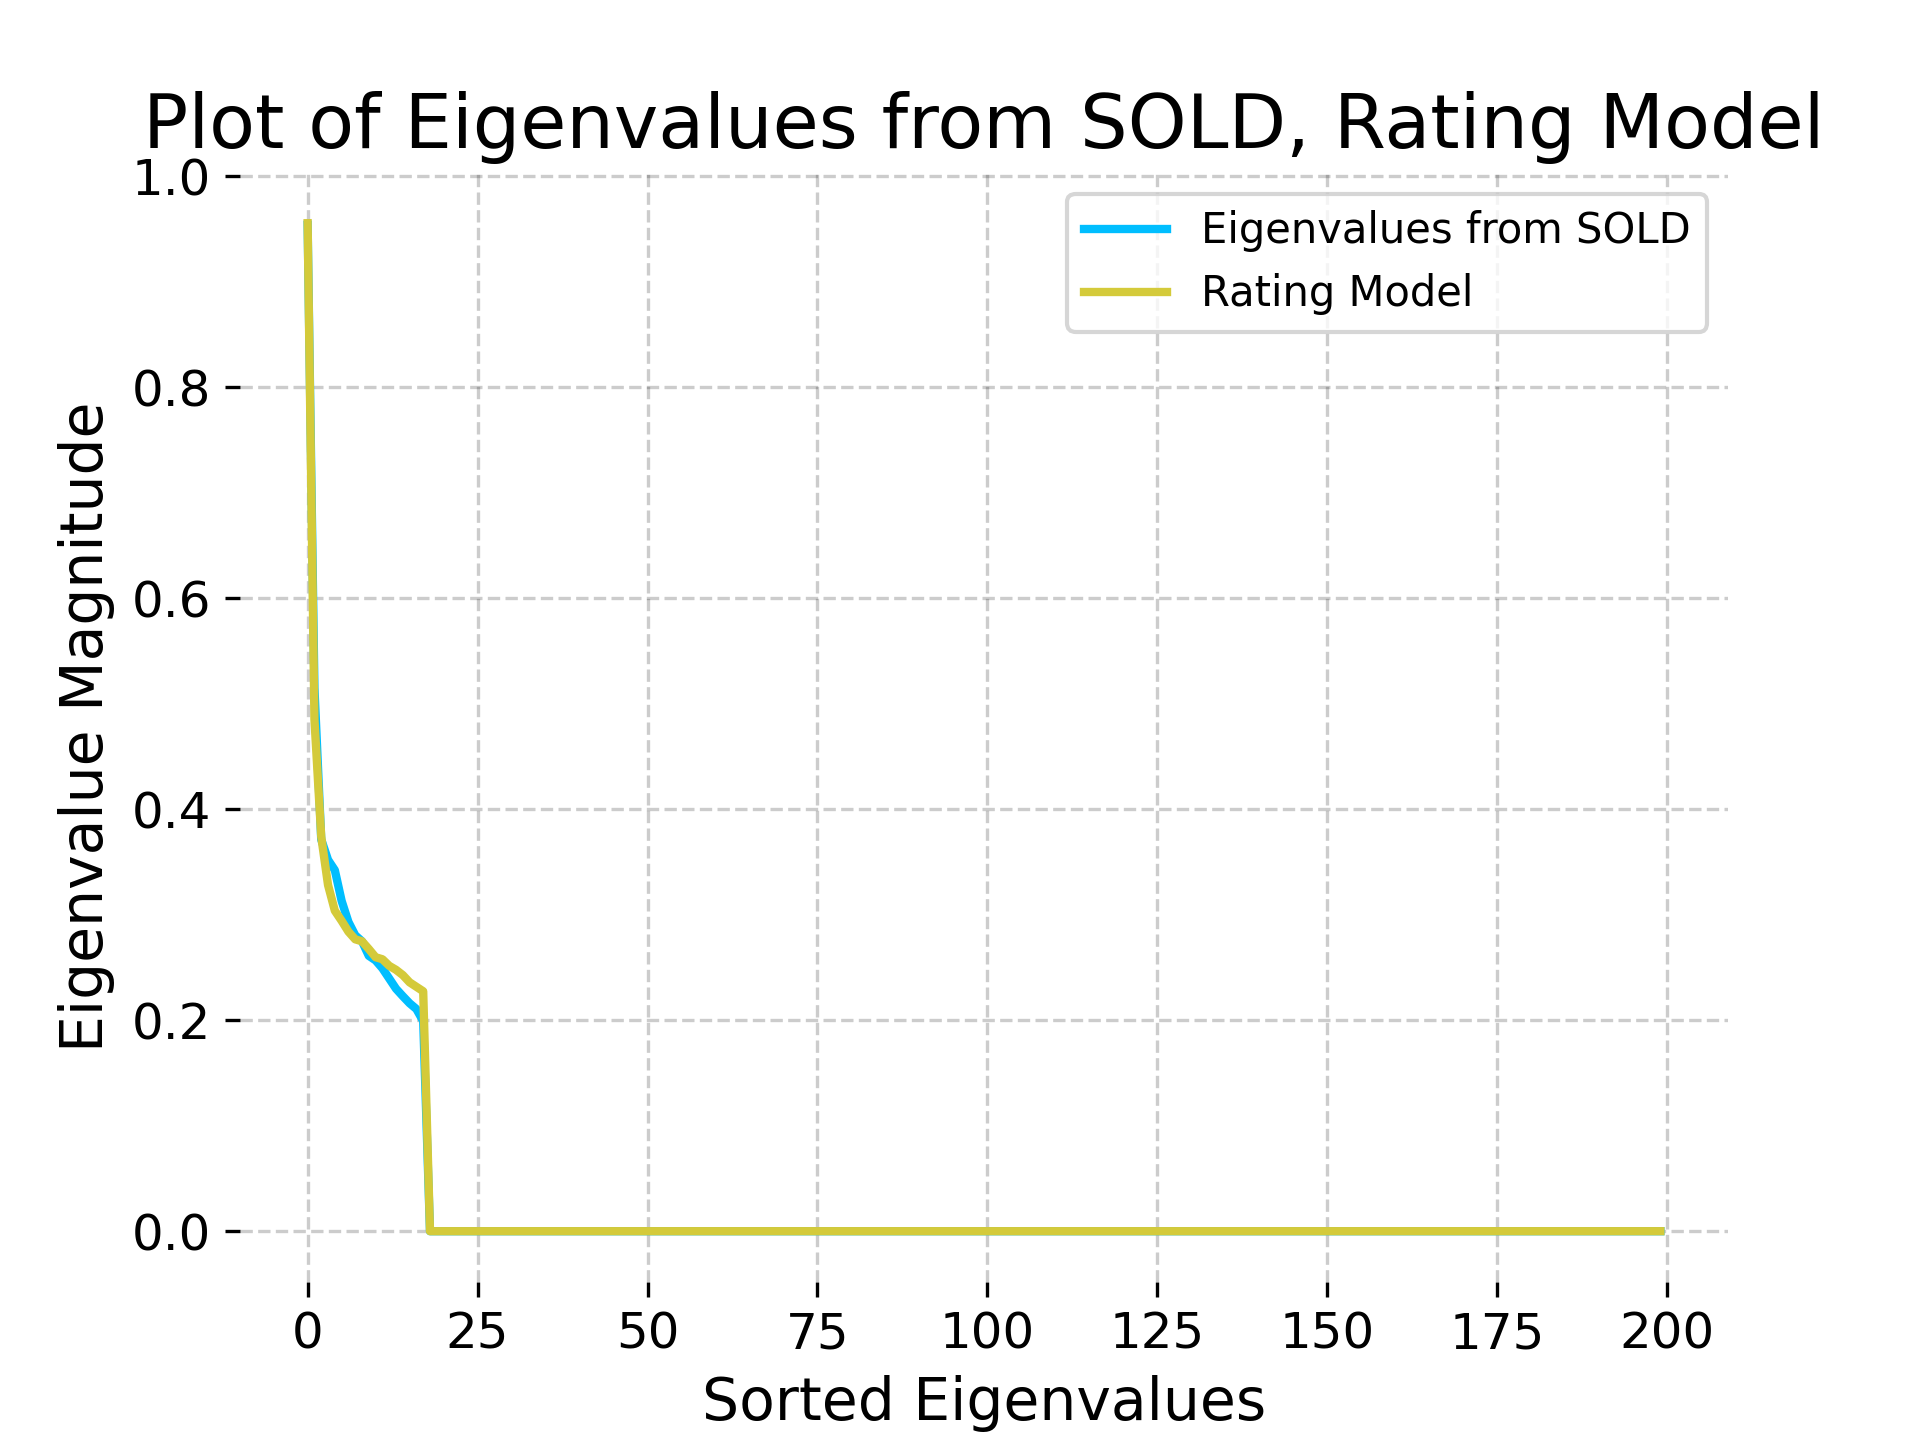
\includegraphics[scale=0.5]{figures/ch03/imgs/movies/sold_eigs.png}
    \caption{Plot of eigenvalues of aforementioned matrix. Notice the drop after $18$ eigenvalues. }
    \label{fig:eig-plot}
\end{figure}

\begin{figure}[H]
    \centering
    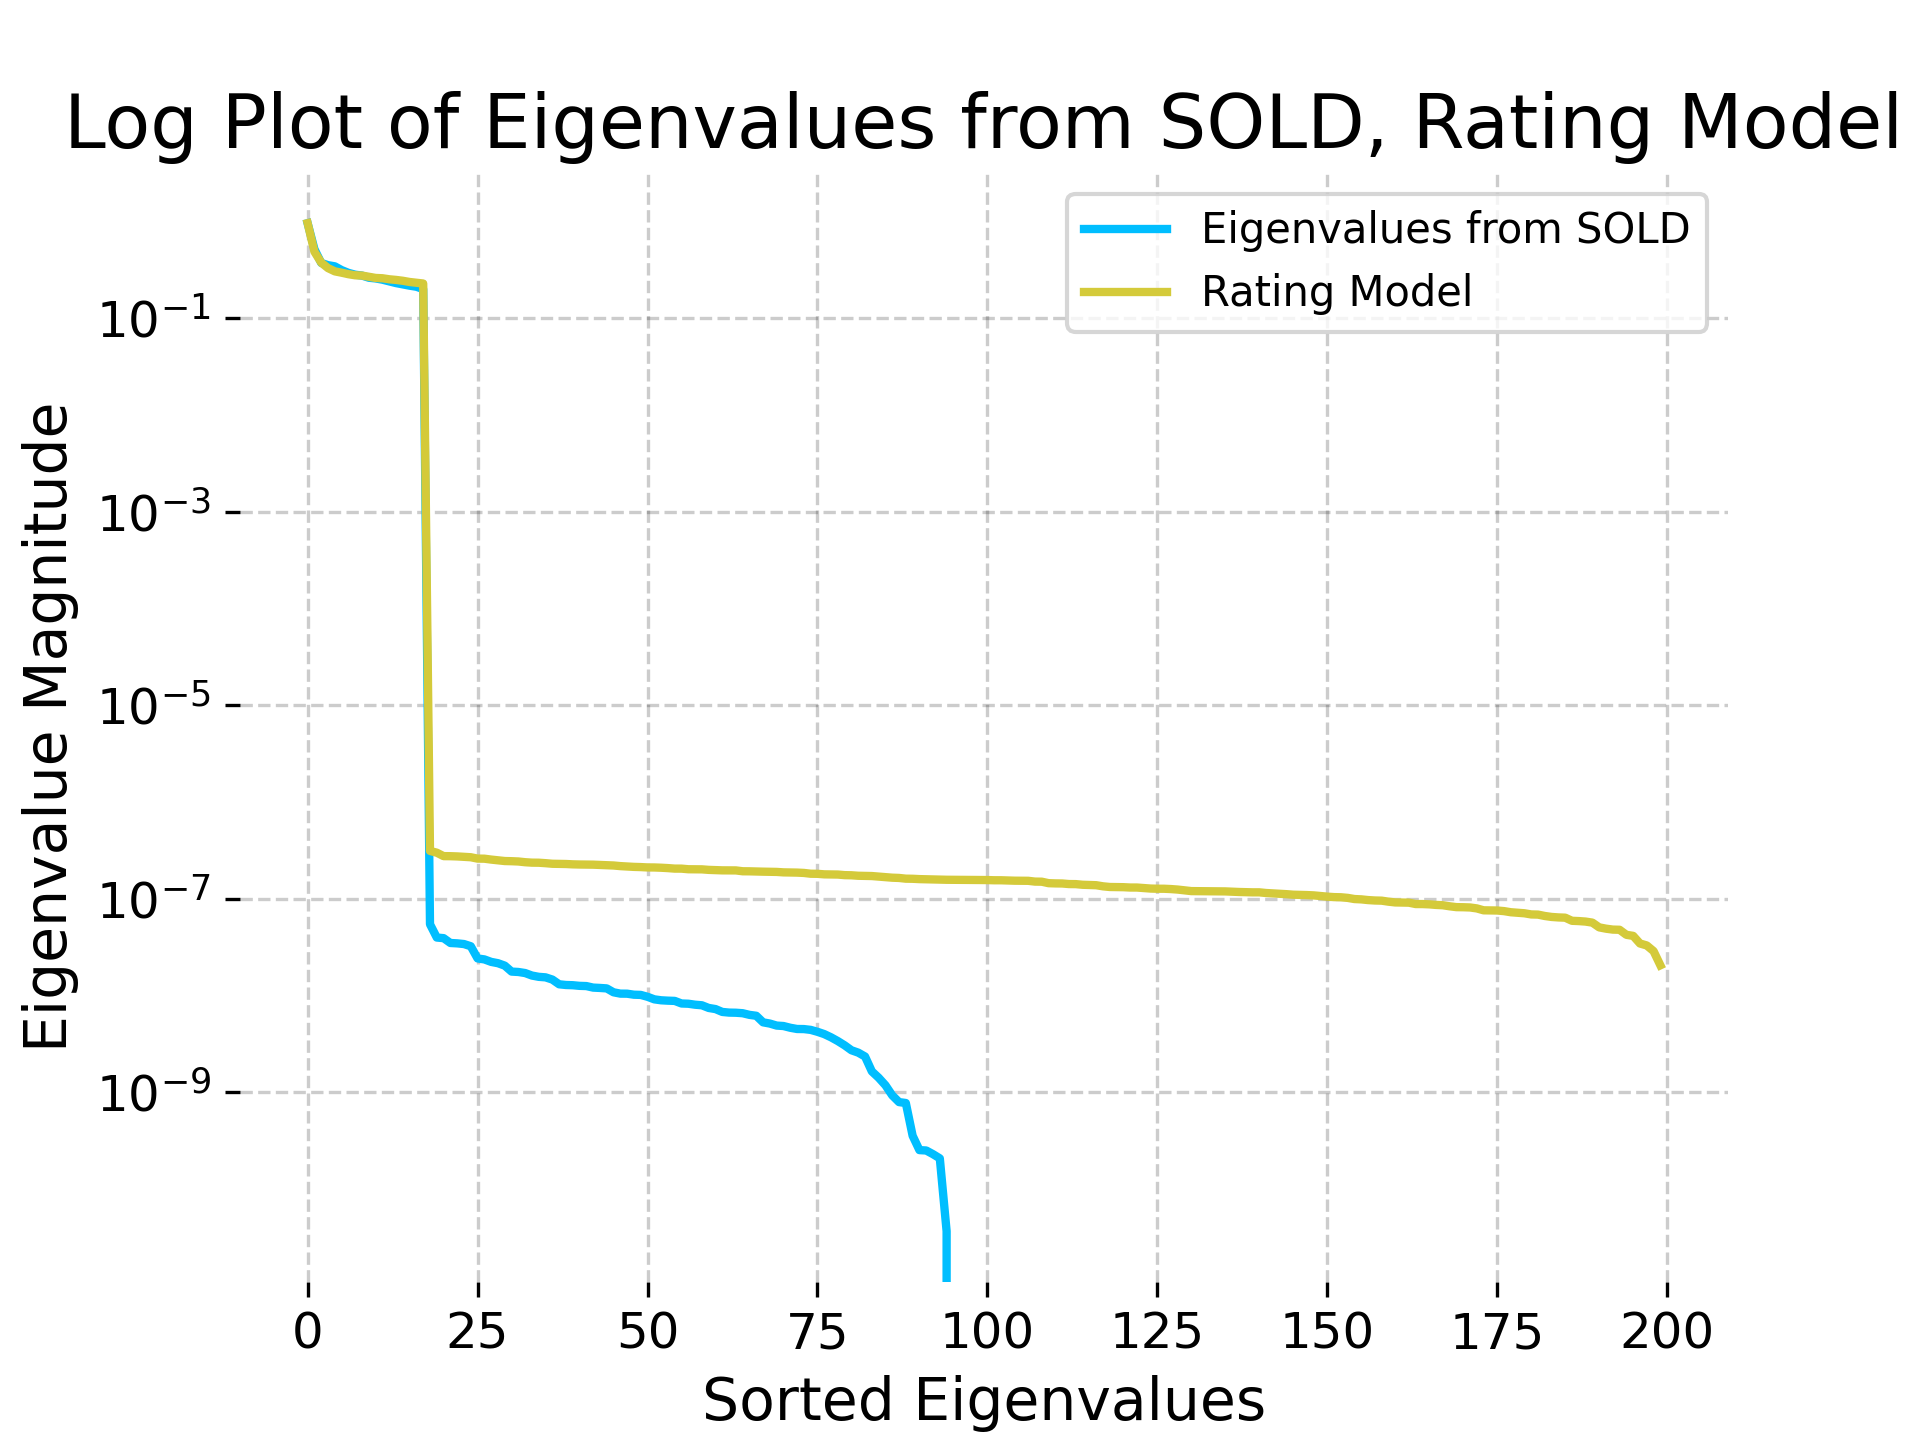
\includegraphics[scale=0.5]{figures/ch03/imgs/movies/sold_eigs_log.png}
    \caption{Log-plot of eigenvalues of aforementioned matrix. Notice the drop after $18$ eigenvalues. }
    \label{fig:eig-log-plot}
\end{figure}

\newpage
\subsection{Simulation Study}
We generate $\BU_*$ with $\BU_{ij} \text{ i.i.d. } \text{Unif}(0,\frac{2.5}{d_K d_A})$. We simulate the hidden labels $\btheta_n \sim \gN(0, d_K^{-1}\BI_{d_K})$, generate feature vectors $\phi(x_{n,h}, a_{n,h}) \sim \gN(0, \BI_{d_A})$ normalized to unit norm, and sample noise $\epsilon_{n,h} \text{ i.i.d. } \gN(0, 0.5^2)$. We use \aigen{Algorithm~\ref{alg:sold}} to estimate $\hat{\BU}$ from the offline dataset $\gD_{\off}$, which consists of $5000$ trajectories of length $20$ each. In accordance with the confidence set determined by \cite{Li_2010}, we choose $\alpha_{1,t} = 0.33\sqrt{d_K\log(1+10T/d_K)}$ and $\alpha_{2,t} = 0.33\sqrt{d_A\log(1+10T/d_A)}$, and share the LinUCB and \aigen{Algorithm~\ref{alg:proball-ucb}} hyperparameters by assigning $\alpha_t=\alpha_{2,t}$. 
\footnote{All experiments were run on a single computer with an Intel i9-13900k CPU, 128GB of RAM, and a NVIDIA RTX 3090 GPU, in no more than an hour in total.}

\begin{figure}[H]
    \centering
    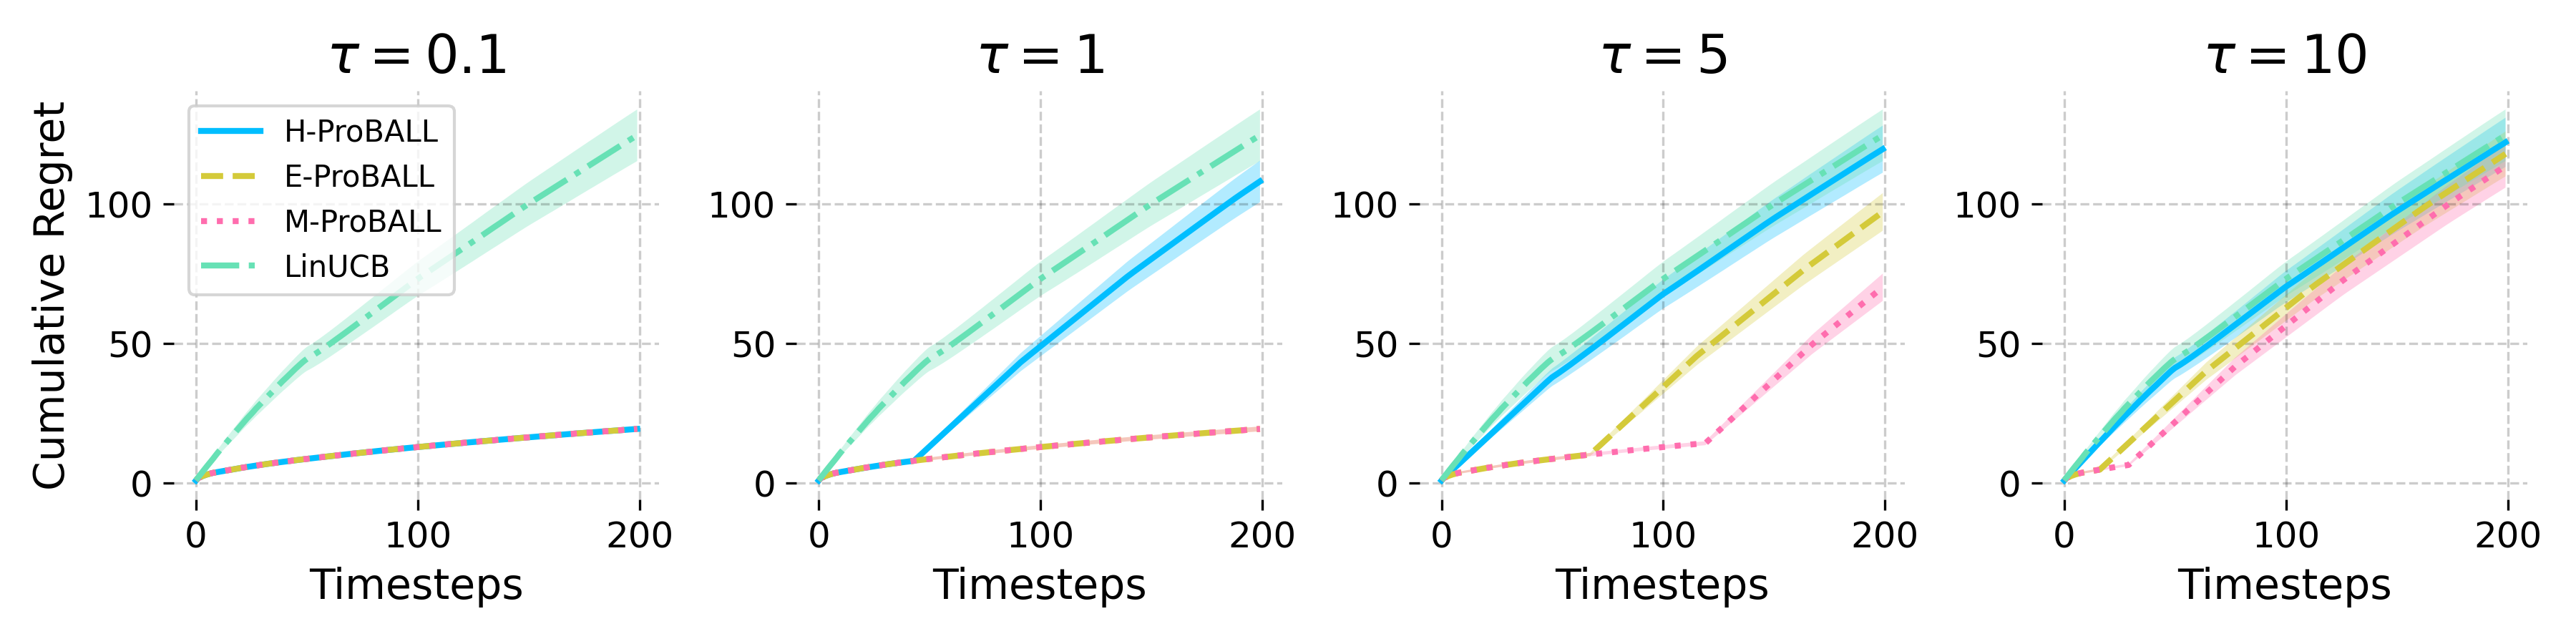
\includegraphics[width=\textwidth]{figures/ch03/imgs/sims/bayes_regret_sims.png}
    \caption{Comparison of \aigen{Algorithm~\ref{alg:proball-ucb}} with LinUCB, for different choices of $\tau$ and confidence bound constructions. All variants perform no worse than LinUCB, with martingale Bernstein performing the best. The shaded area depicts $1$-standard error confidence intervals over $30$ trials.}
    \label{fig:regret-sims-ablation}
\end{figure}

\newpage
\subsection{MovieLens}

MovieLens \citep{movielens} is a large-scale movie recommendation dataset comprising $6040$ users and $3883$ movies, where each user may rate one or more movies. Like \cite{hong2020latent}, we filter the dataset to include only movies rated by at least $200$ users and vice-versa.
%-- but we get slightly different numbers for the remaining users ($1589$) and movies ($1426$) post-filtering.
We factor the sparse rating matrix into user parameters $\bbeta$ and movie features $\Phi$ using the probabilistic matrix factorization algorithm of \cite{mnih2007pmf}, using nuclear norm regularization so that the rank of $\bbeta$ is $d_K=18$. However, we consider a much higher dimensional problem than \cite{hong2020latent} do -- we let $d_A = 200$ so $\bbeta\in \Real^{1589\times 200}, \Phi \in \Real^{200 \times 1426}$. At each round for user $i$, the agent chooses between $20$ movies of different genres with features $\Phi_{a_1},...,\Phi_{a_{20}}$, and has to recommend the best movie presented to it to maximize the user's rating of the movie. We generate rewards for recommending movie $j$ to user $i$ by $\bbeta_{i}^T\Phi_j + \epsilon_{ij}, \epsilon_{ij} \text{ i.i.d. } \gN(0, 0.5)$. 

Our hyperparameters are chosen and varied just as in the simulation study. To reproduce the methods of \cite{hong2020latent}, we cluster the user features into $d_K$ clusters using k-means, and provide mUCB and mmUCB with the mean vectors of each cluster as latent models. We initialize \aigen{Algorithm~\ref{alg:proball-ucb}} with a subspace estimated with an unregularized variant of \aigen{Algorithm~\ref{alg:sold}}, that uses pseudo-inverses instead of inverses, because of difficulties in finding an appropriate regularization parameter for this large, noisy, and high-dimensional dataset. The subspace was estimated from $5000$ trajectories of length $50$ simulated from the reward model and the uniform behavior policy. Note that we assign $\Delta_{\off}$ for $\epsilon$ in mmUCB, as this is their tolerance parameter for model misspecification.

\begin{figure}[H]
    \centering
    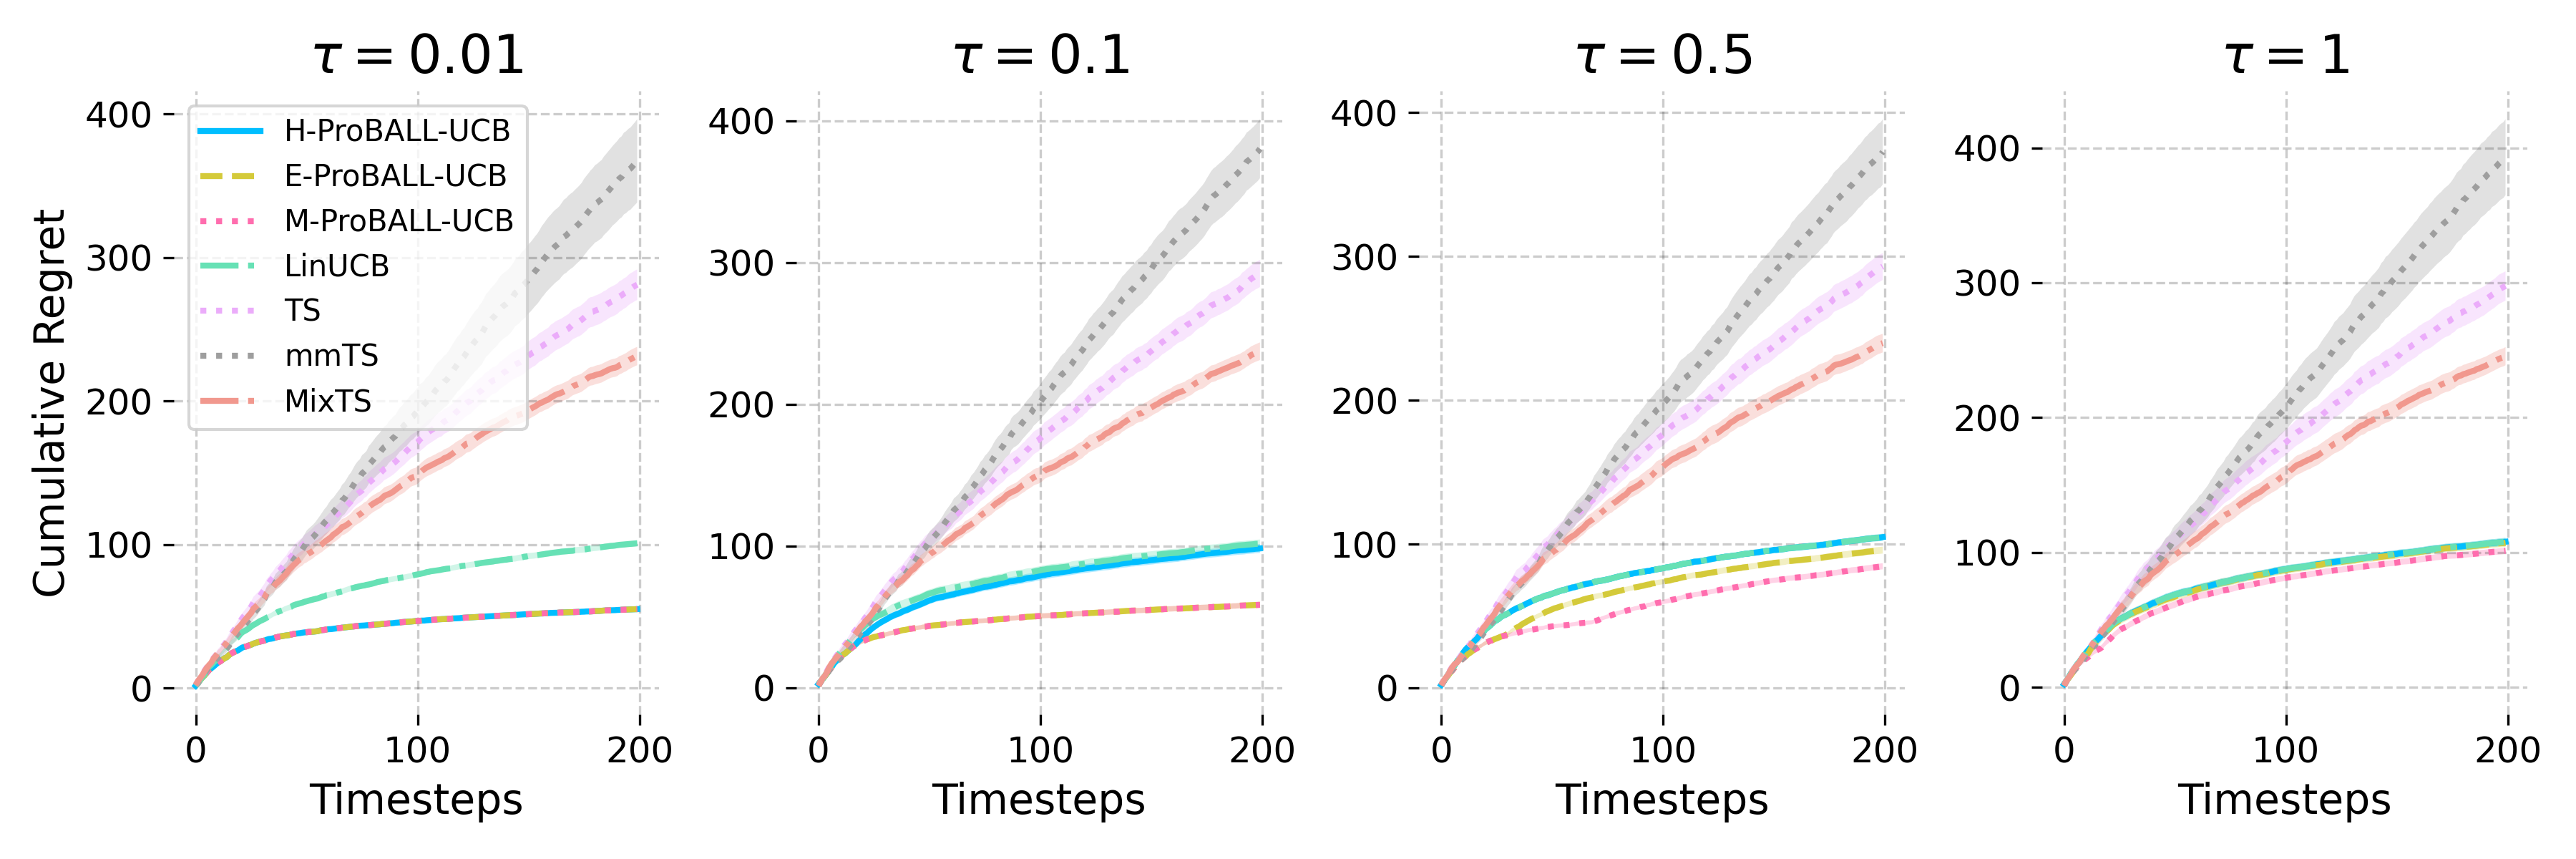
\includegraphics[scale=0.5]{figures/ch03/imgs/movies/bayes_regret_comparison_sold_movies.png}
    \caption{Comparison of \aigen{Algorithm~\ref{alg:proball-ucb}} with LinUCB and TS algorithms, for different choices of $\tau$ and confidence bound constructions. All variants perform no worse than LinUCB and outperform the TS algorithms, with martingale Bernstein performing the best. The shaded area depicts $1$-standard error confidence intervals over $30$ trials.}
    \label{fig:regret-sims} 
\end{figure}



\begin{figure}[H]
    \centering
    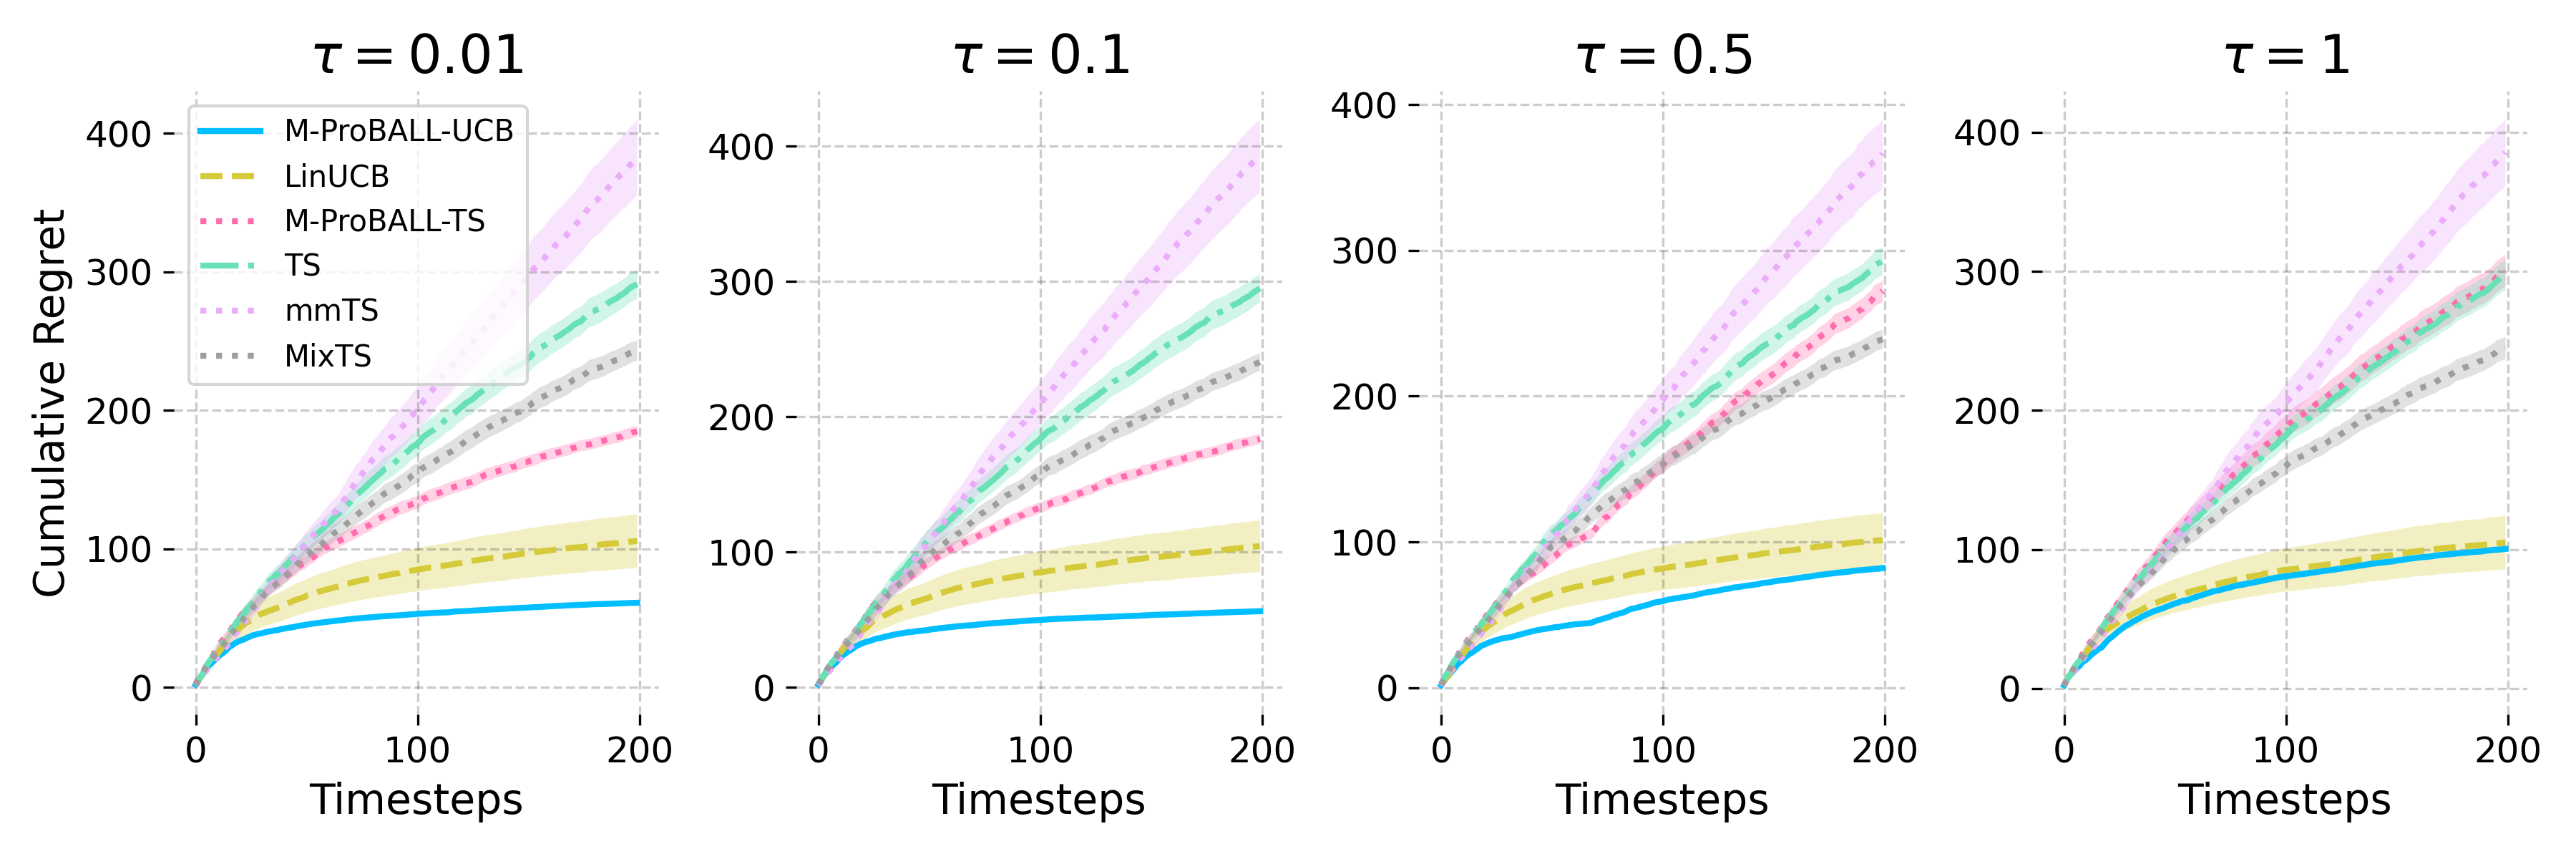
\includegraphics[scale=0.5]{figures/ch03/imgs/movies/bayes_regret_ucb_ts_sold_movies.png}
    \caption{Comparison of \aigen{Algorithm~\ref{alg:proball-ucb}} and \aigen{projected confidence-ball Thompson sampling (Algorithm~\ref{alg:proball-ts})} initialized with \aigen{Algorithm~\ref{alg:sold}} against LinUCB, TS, MixTS, and mmTS, for different choices of $\tau$ and confidence bound constructions. \aigen{Algorithm~\ref{alg:proball-ucb}} outperforms LinUCB, and \aigen{projected confidence-ball Thompson sampling (Algorithm~\ref{alg:proball-ts})} outperforms MixTS and mmTS. Shaded area depicts $1$-standard error confidence intervals over $30$ trials with fresh $\btheta$. The confidence intervals on regret thus account for the variation in frequentist regret for changing $\btheta$.}
    \label{fig:regret-movies-ucb-ts}
\end{figure}

\newpage
\begin{minipage}{\textwidth}
\subsubsection{UCB Algorithms}

\begin{figure}[H]
    \centering
    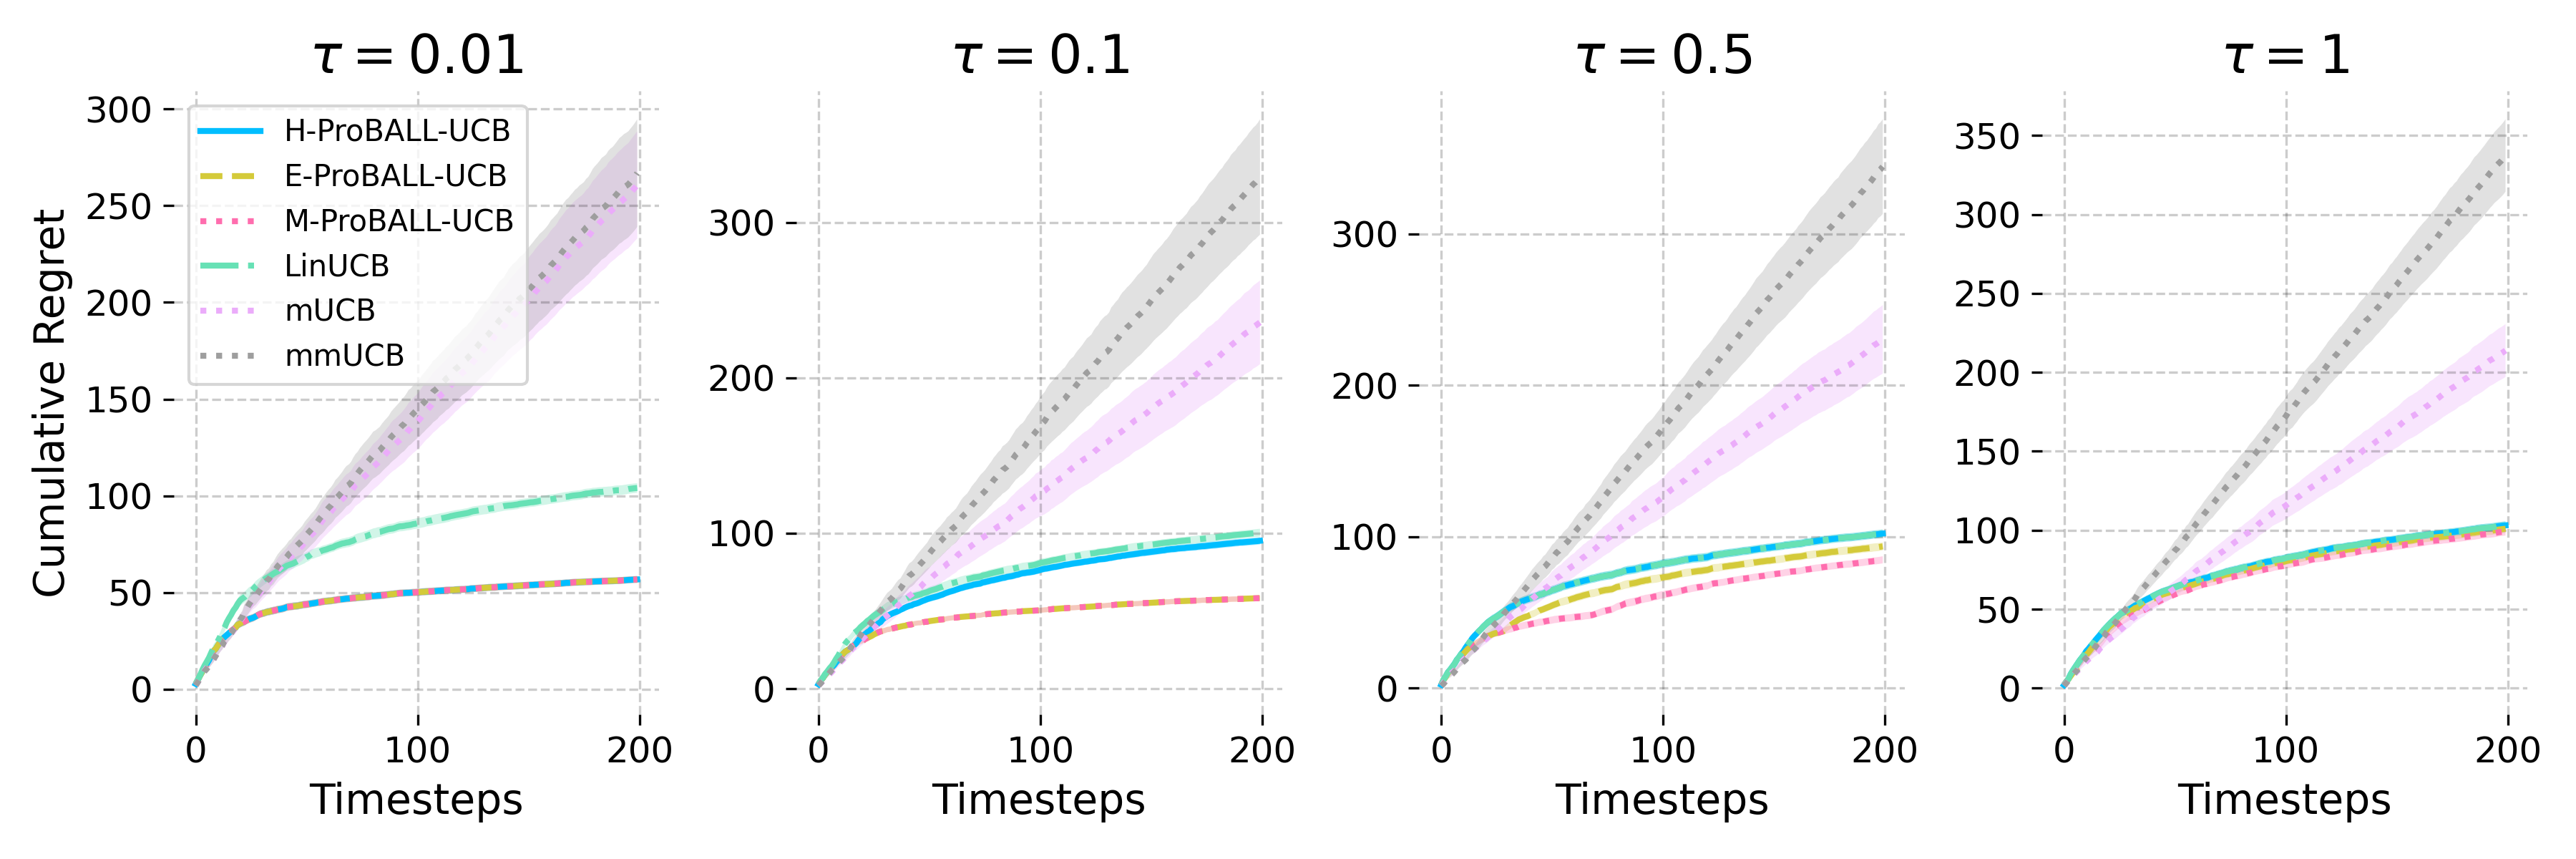
\includegraphics[scale=0.5]{figures/ch03/imgs/movies/bayes_regret_ucbs_sold_movies.png}
    \caption{Comparison of \aigen{Algorithm~\ref{alg:proball-ucb}} initialized with \aigen{Algorithm~\ref{alg:sold}} against LinUCB, mUCB, and mmUCB, for different choices of $\tau$ and confidence bound constructions, in terms of regret. All variants of \aigen{Algorithm~\ref{alg:proball-ucb}} perform no worse than LinUCB, and outperform mUCB and mmUCB. Shaded area depicts $1$-standard error confidence intervals over 30 trials with fresh $\theta$. The confidence intervals on regret thus account for the variation in frequentist regret for changing $\theta$.}
    \label{fig:movie-regret-ucbs-sold}
\end{figure}

\begin{figure}[H]
    \centering
    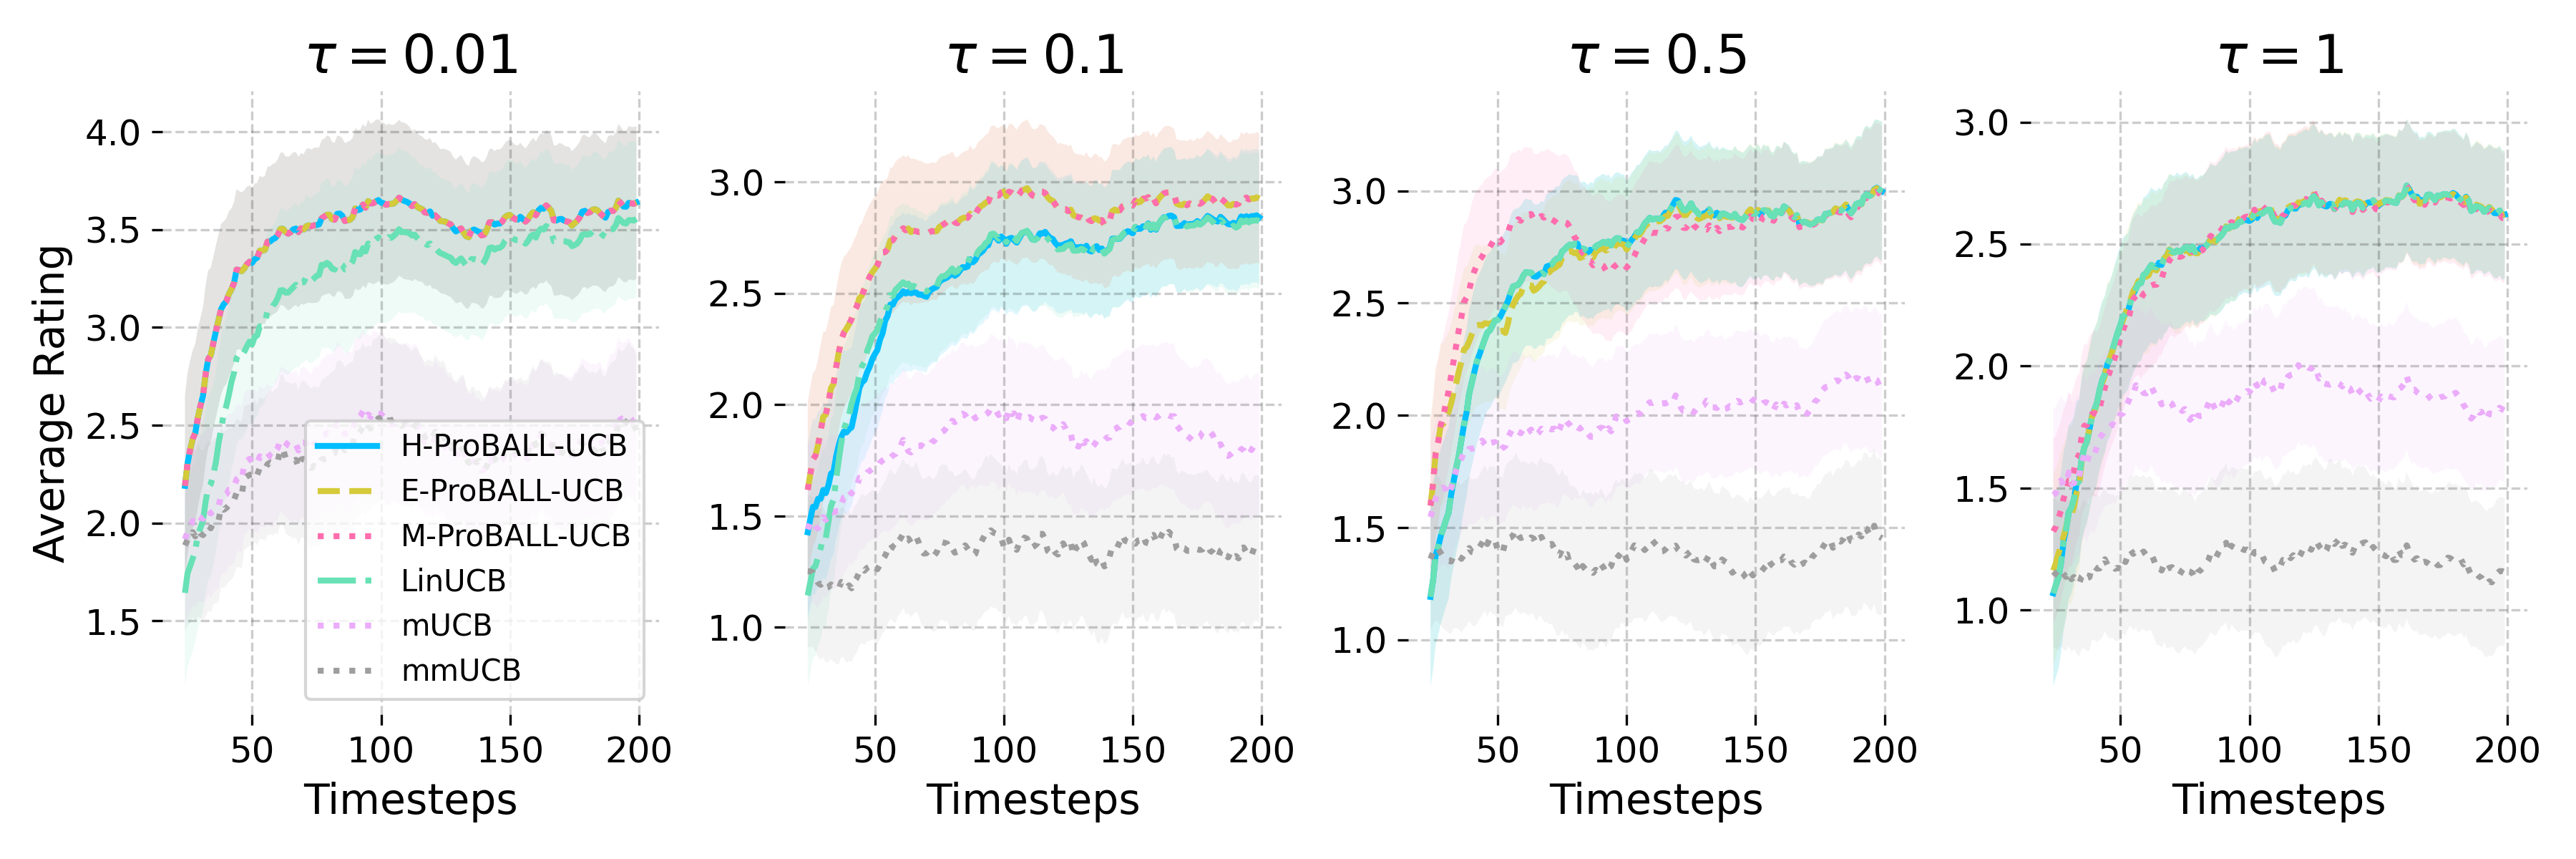
\includegraphics[scale=0.5]{figures/ch03/imgs/movies/bayes_rating_ucbs_sold_movies.png}
    \caption{Comparison of \aigen{Algorithm~\ref{alg:proball-ucb}} initialized with \aigen{Algorithm~\ref{alg:sold}} against LinUCB, mUCB, and mmUCB, for different choices of $\tau$ and confidence bound constructions, in terms of rolling average rating over $25$ timesteps. \aigen{Algorithm~\ref{alg:proball-ucb}} performs no worse than LinUCB, and outperforms mUCB and mmUCB. }
    \label{fig:movie-rating-ucbs-sold}
\end{figure}
\end{minipage}

\newpage
\begin{minipage}{\textwidth}
\subsubsection{TS Algorithms}\label{app:proball-ts}

\begin{figure}[H]
    \centering
    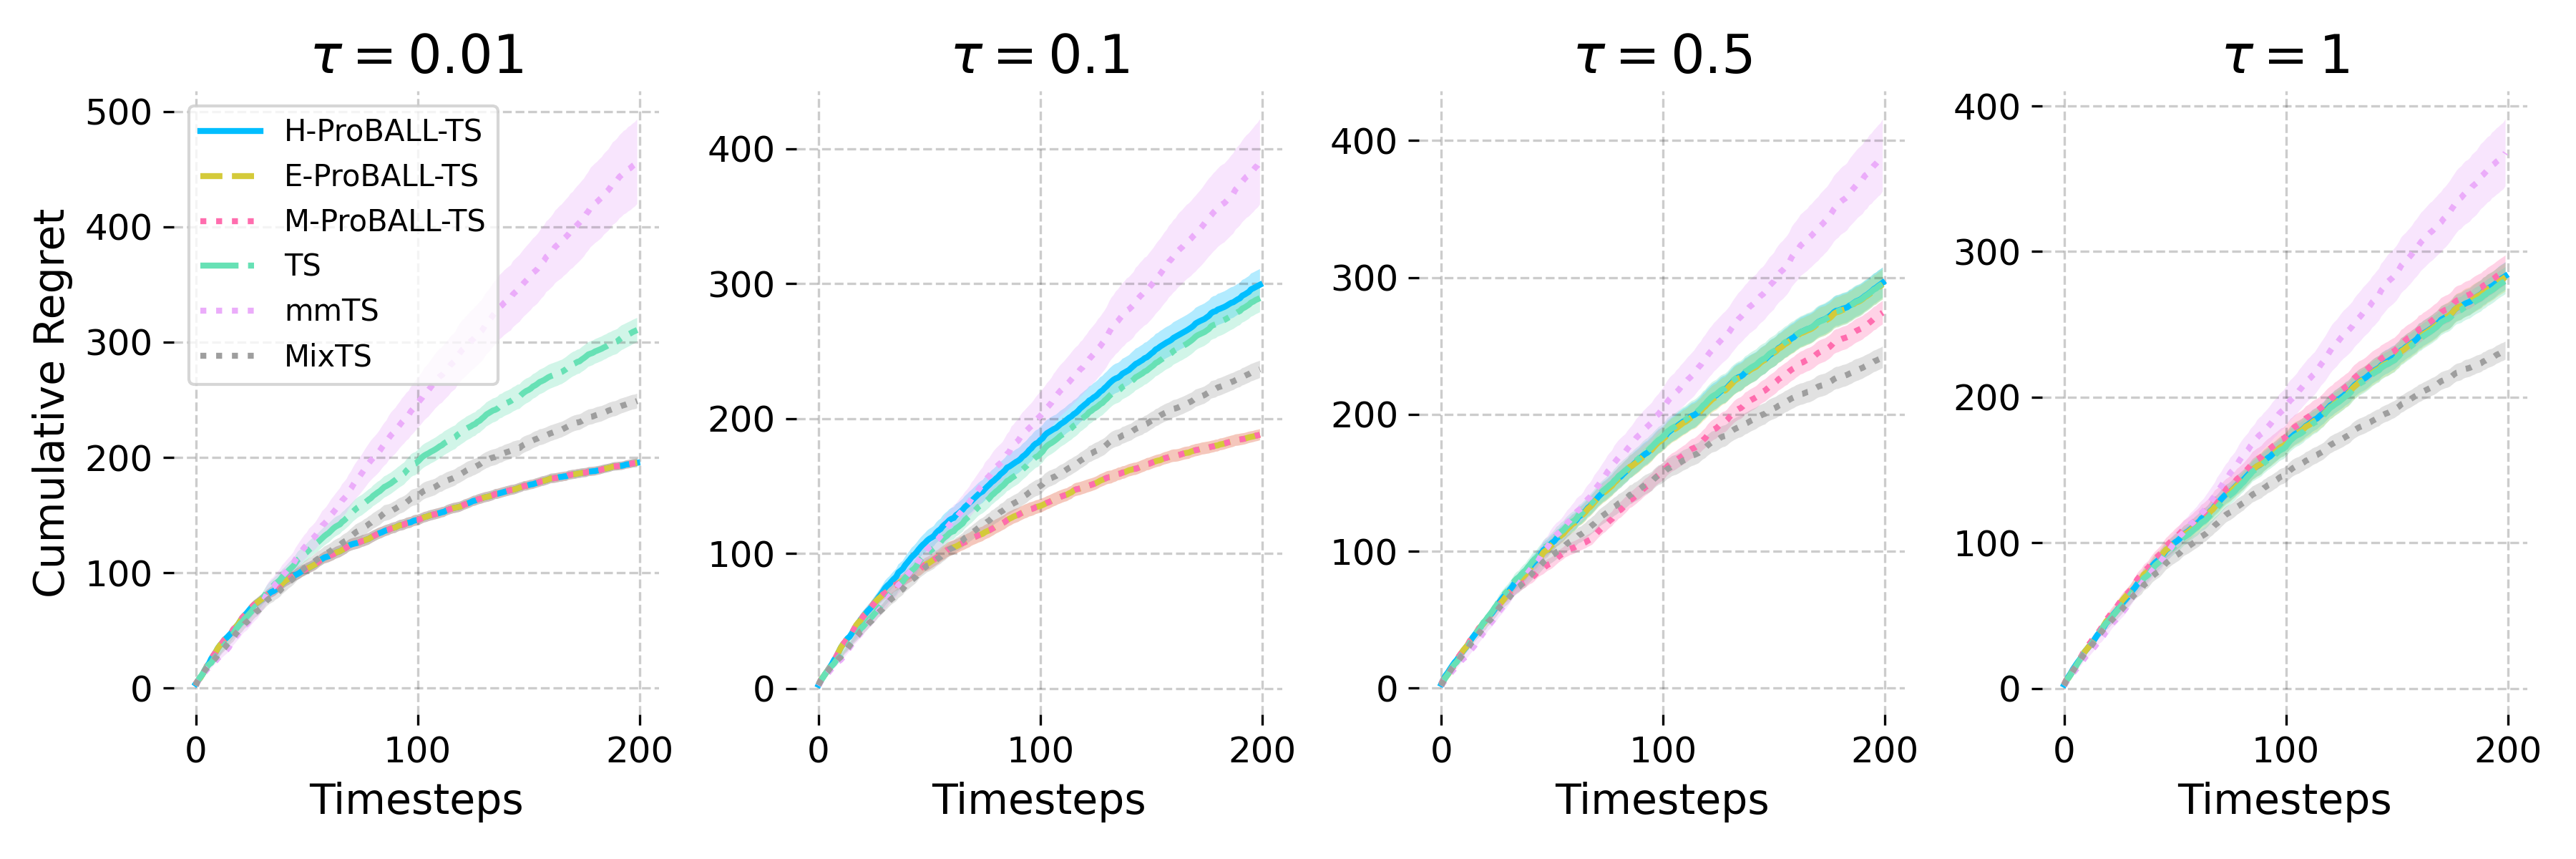
\includegraphics[scale=0.5]{figures/ch03/imgs/movies/bayes_regret_ts_sold_movies.png}
    \caption{Comparison of \aigen{projected confidence-ball Thompson sampling (Algorithm~\ref{alg:proball-ts})} initialized with \aigen{Algorithm~\ref{alg:sold}} against TS, mmTS, and MixTS, for different choices of $\tau$ and confidence bound constructions, in terms of regret. All variants of \aigen{projected confidence-ball Thompson sampling (Algorithm~\ref{alg:proball-ts})} outperform TS, mmTS, and MixTS. }
    \label{fig:movie-regret-ts-sold}
\end{figure}

\begin{figure}[H]
    \centering
    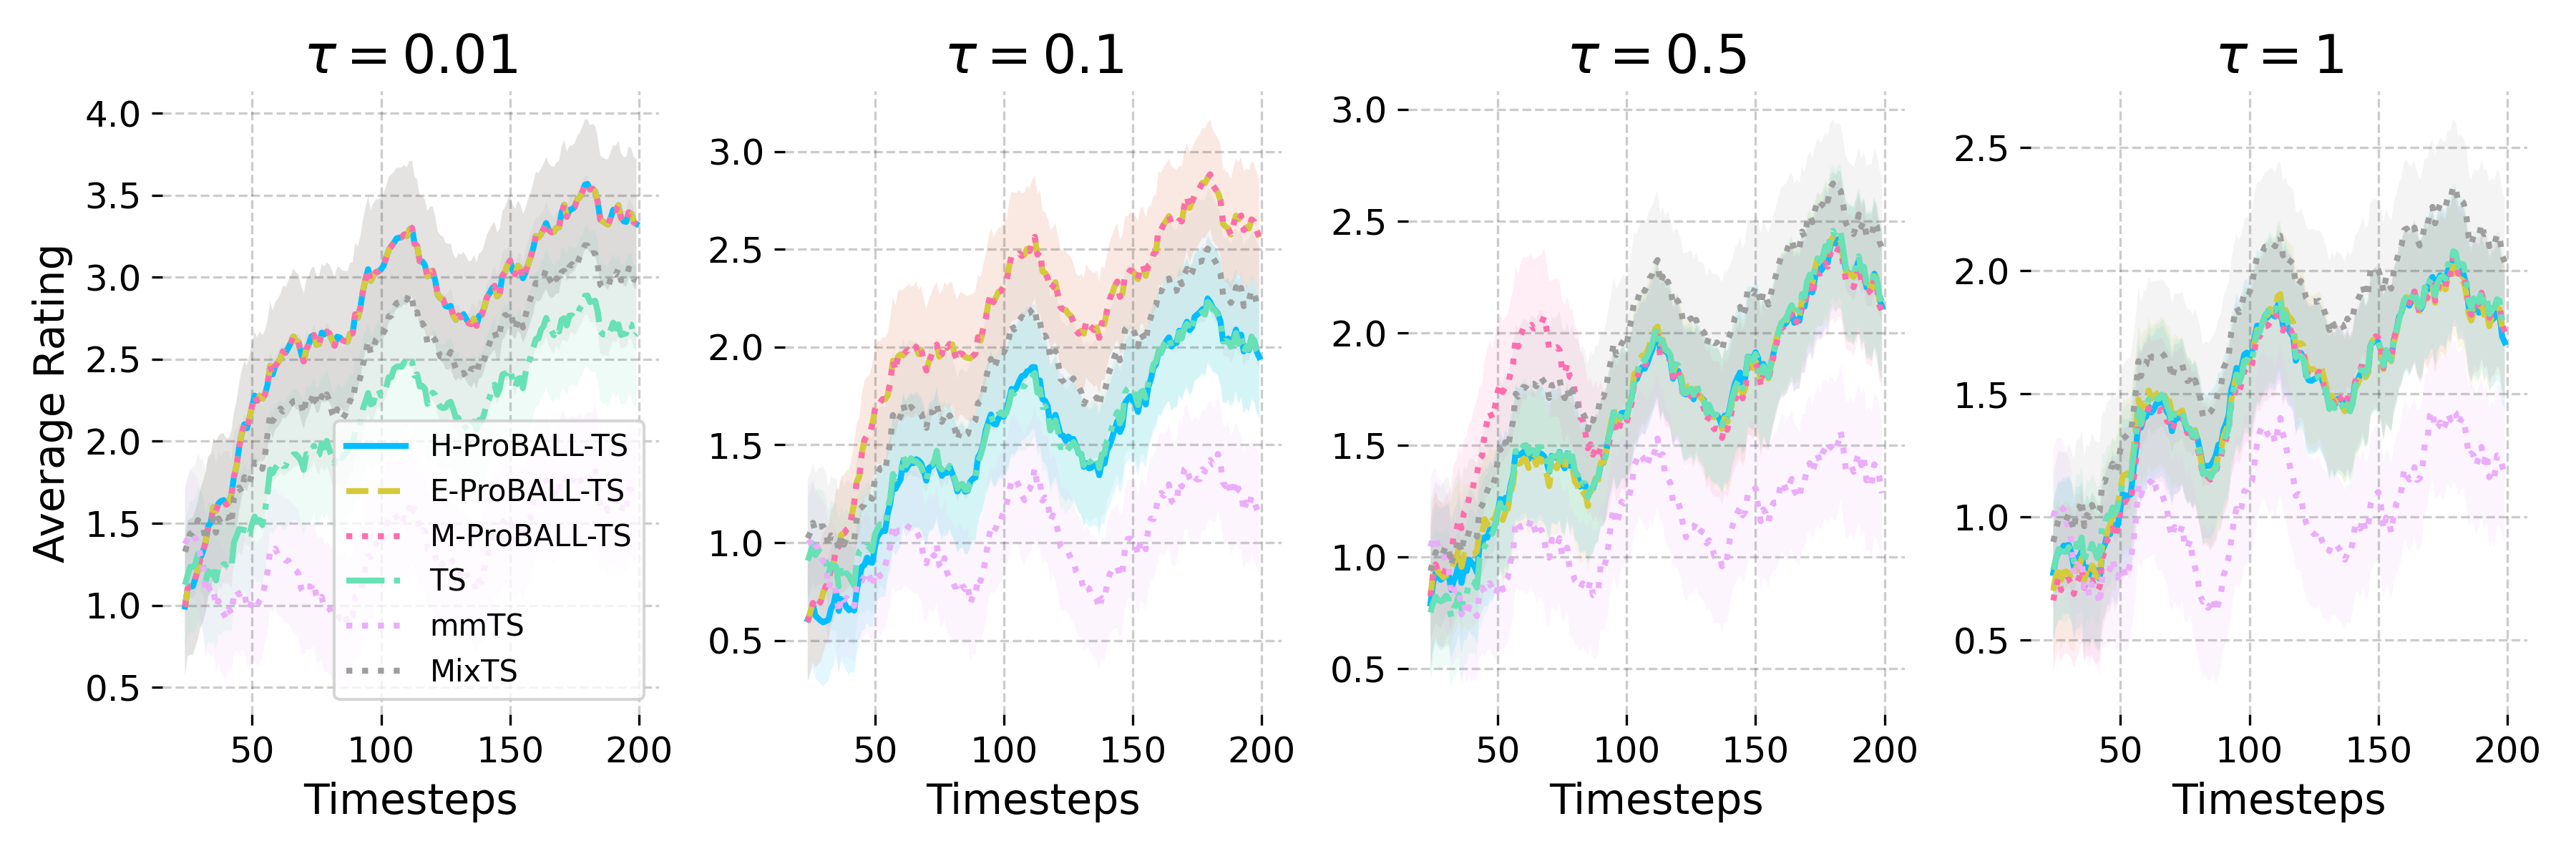
\includegraphics[scale=0.5]{figures/ch03/imgs/movies/bayes_rating_ts_sold_movies.png}
    \caption{Comparison of \aigen{projected confidence-ball Thompson sampling (Algorithm~\ref{alg:proball-ts})} initialized with \aigen{Algorithm~\ref{alg:sold}} against TS, mmTS, and MixTS, for different choices of $\tau$ and confidence bound constructions, in terms of rolling average rating over $25$ timesteps. All variants of \aigen{projected confidence-ball Thompson sampling (Algorithm~\ref{alg:proball-ts})} outperform TS, mmTS, and MixTS. Shaded area depicts $1$-standard error confidence intervals over 30 trials with fresh $\theta$. The confidence intervals on regret thus account for the variation in frequentist regret for changing $\theta$. }
    \label{fig:movie-rating-ts-sold}
\end{figure}
\end{minipage}

\newpage
\begin{minipage}{\textwidth}
\subsubsection{Comparison Against Low-Dimensional Ground Truth Subspaces}


\begin{figure}[H]
    \centering
    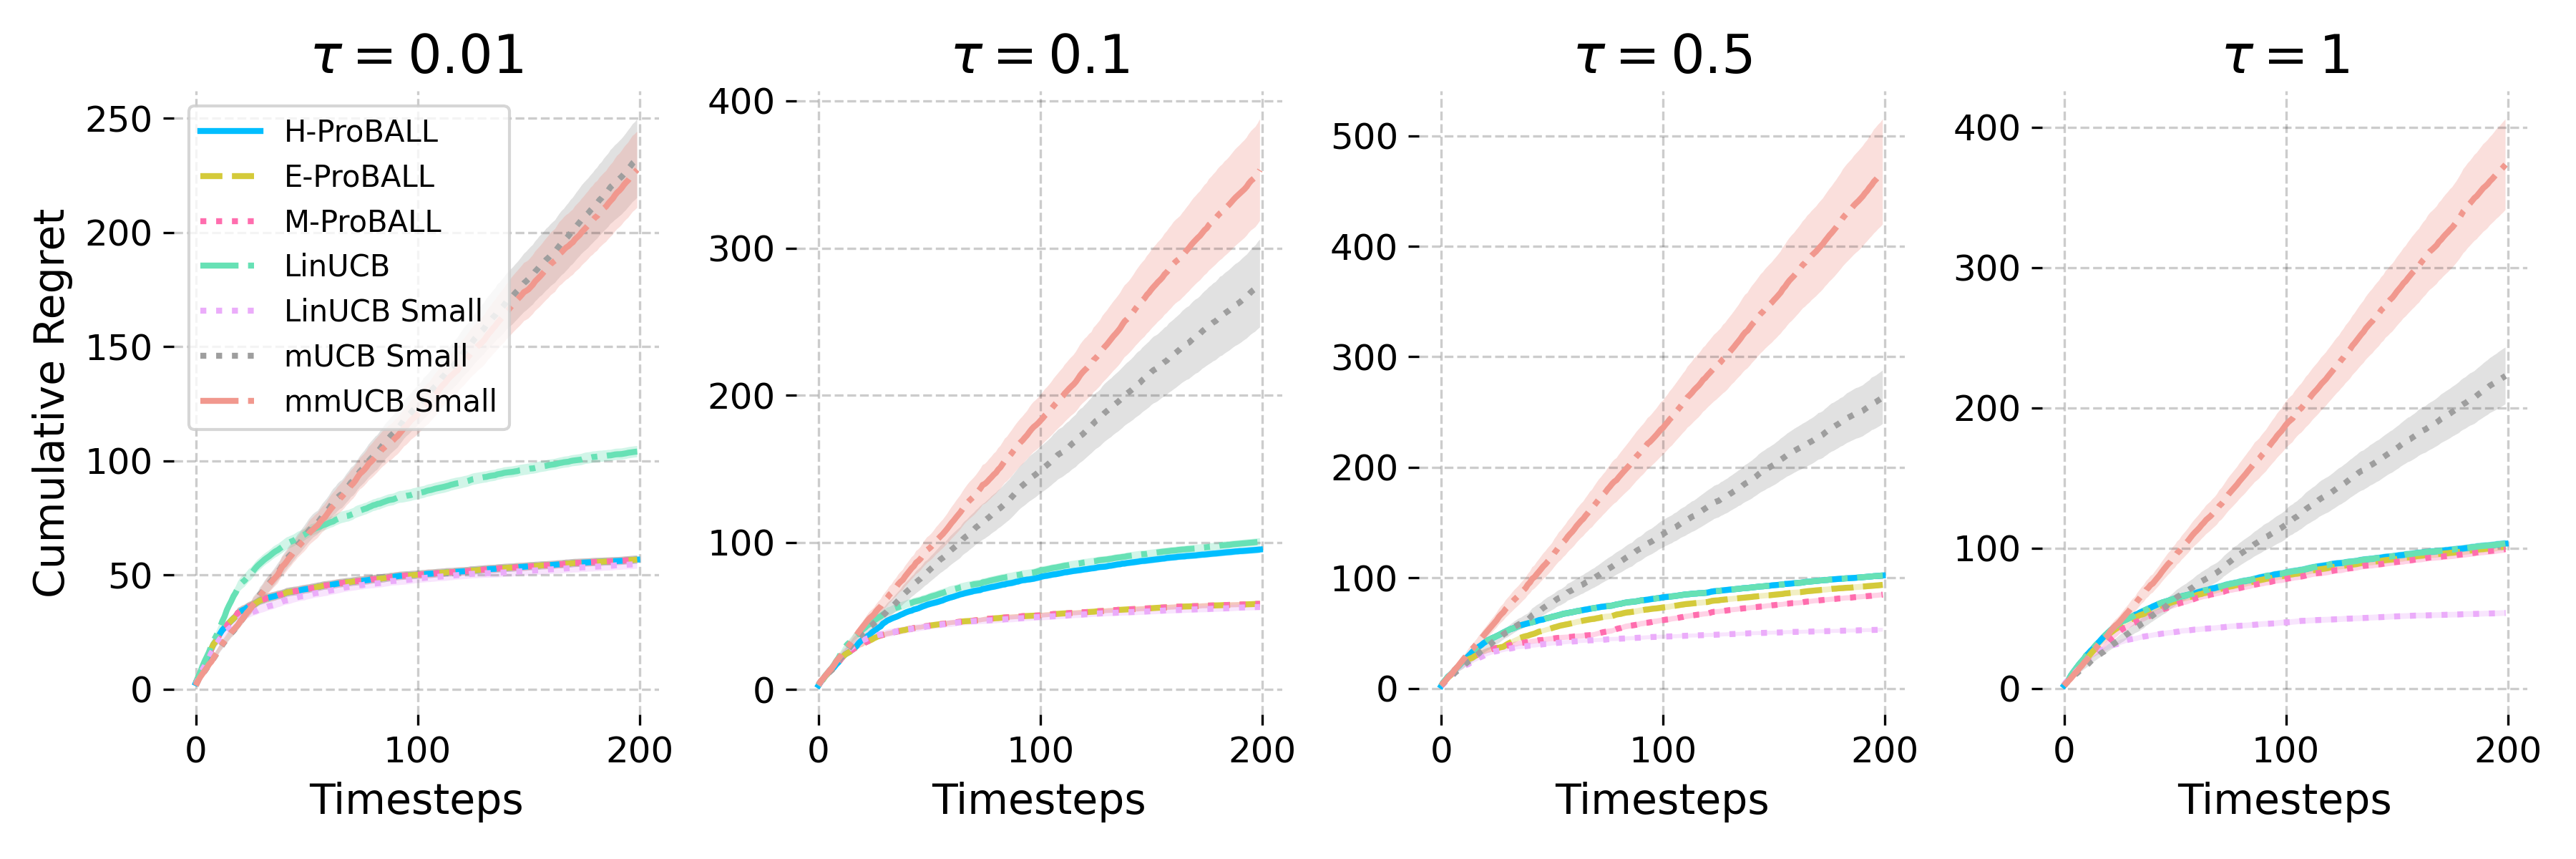
\includegraphics[scale=0.55]{figures/ch03/imgs/movies/bayes_regret_small_sold_movies.png}
    \caption{Comparison of \aigen{Algorithm~\ref{alg:proball-ucb}} initialized with \aigen{Algorithm~\ref{alg:sold}} against LinUCB, mUCB, and mmUCB on low-dimensional ground-truth features, for different choices of $\tau$ and confidence bound constructions. When $\tau$ is small enough, all variants of \aigen{Algorithm~\ref{alg:proball-ucb}} perform no worse than low-dimensional LinUCB, and outperform mUCB and mmUCB, on ground truth features. This showcases the efficacy of \aigen{Algorithm~\ref{alg:sold}}, and demonstrates that we recover subspaces that are just as good as ground-truth. Shaded area depicts $1$-standard error confidence intervals over 30 trials with fresh $\theta$. The confidence intervals on regret thus account for the variation in frequentist regret for changing $\theta$.}
    \label{fig:movie-regret-no-sold}
\end{figure}



\begin{figure}[H]
    \centering
    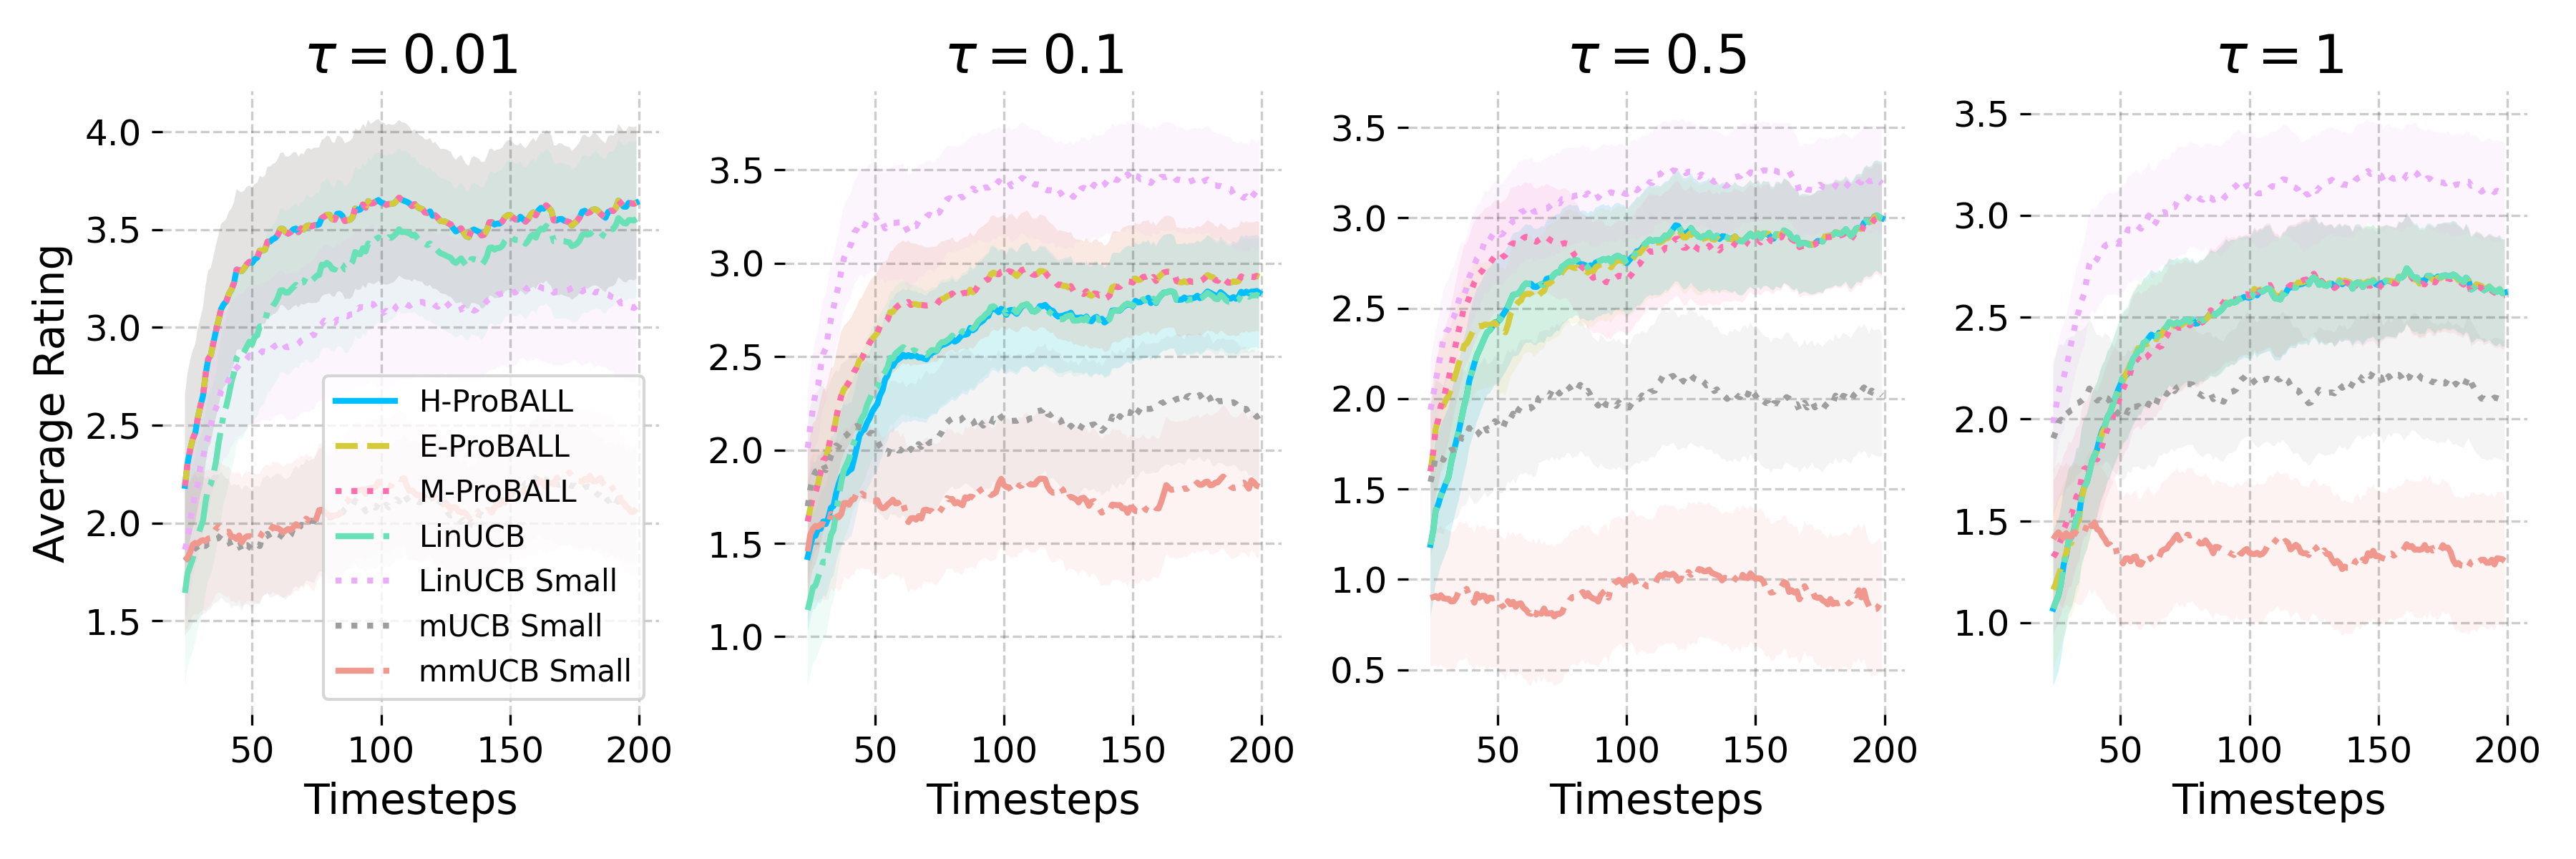
\includegraphics[scale=0.55]{figures/ch03/imgs/movies/bayes_rating_small_sold_movies.png}
    \caption{Comparison of \aigen{Algorithm~\ref{alg:proball-ucb}} initialized with \aigen{Algorithm~\ref{alg:sold}} against LinUCB, mUCB, and mmUCB on low-dimensional ground-truth features, for different choices of $\tau$ and confidence bound constructions. When $\tau$ is small enough, all variants of \aigen{Algorithm~\ref{alg:proball-ucb}} perform no worse than low-dimensional LinUCB, and outperform mUCB and mmUCB, on ground truth features. This showcases the efficacy of \aigen{Algorithm~\ref{alg:sold}}, and demonstrates that we recover subspaces that are just as good as ground-truth. Shaded area depicts $1$-standard error confidence intervals over 30 trials with fresh $\theta$. The confidence intervals on regret thus account for the variation in frequentist regret for changing $\theta$.}
    \label{fig:movie-rating-no-sold}
\end{figure}
\end{minipage}

\begin{minipage}{\textwidth}
   
\subsubsection{No Usage of \aigen{Algorithm~\ref{alg:sold}}}

\begin{figure}[H]
    \centering
    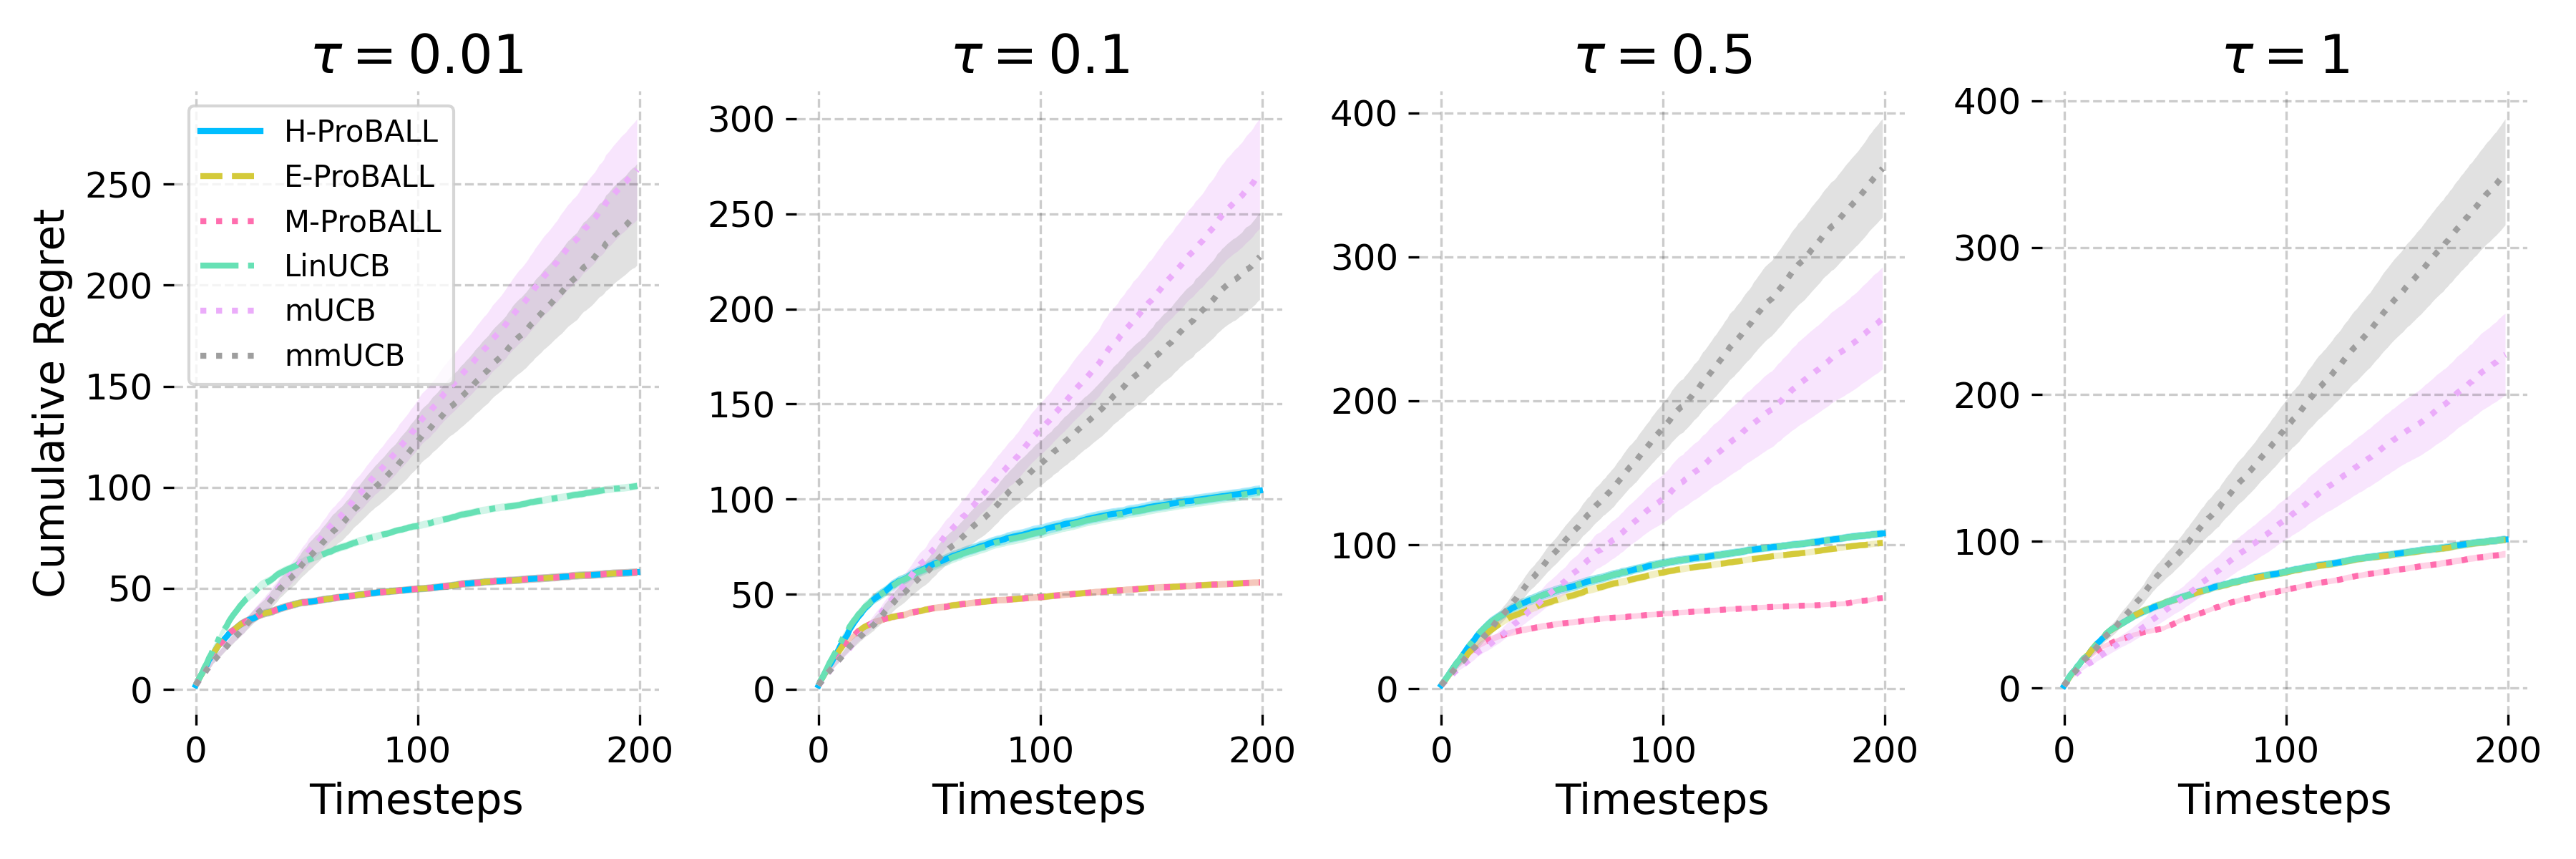
\includegraphics[scale=0.55]{figures/ch03/imgs/movies/bayes_regret_movies.png}
    \caption{Comparison of \aigen{Algorithm~\ref{alg:proball-ucb}} initialized with ground truth subspaces against LinUCB, mUCB, and mmUCB, for different choices of $\tau$ and confidence bound constructions. All variants of \aigen{Algorithm~\ref{alg:proball-ucb}} perform no worse than LinUCB, and outperform mUCB and mmUCB. Shaded area depicts $1$-standard error confidence intervals over 30 trials with fresh $\theta$. The confidence intervals on regret thus account for the variation in frequentist regret for changing $\theta$.}
    \label{fig:movie-regret-no-sold-ts}
\end{figure}
\begin{figure}[H]
    \centering
    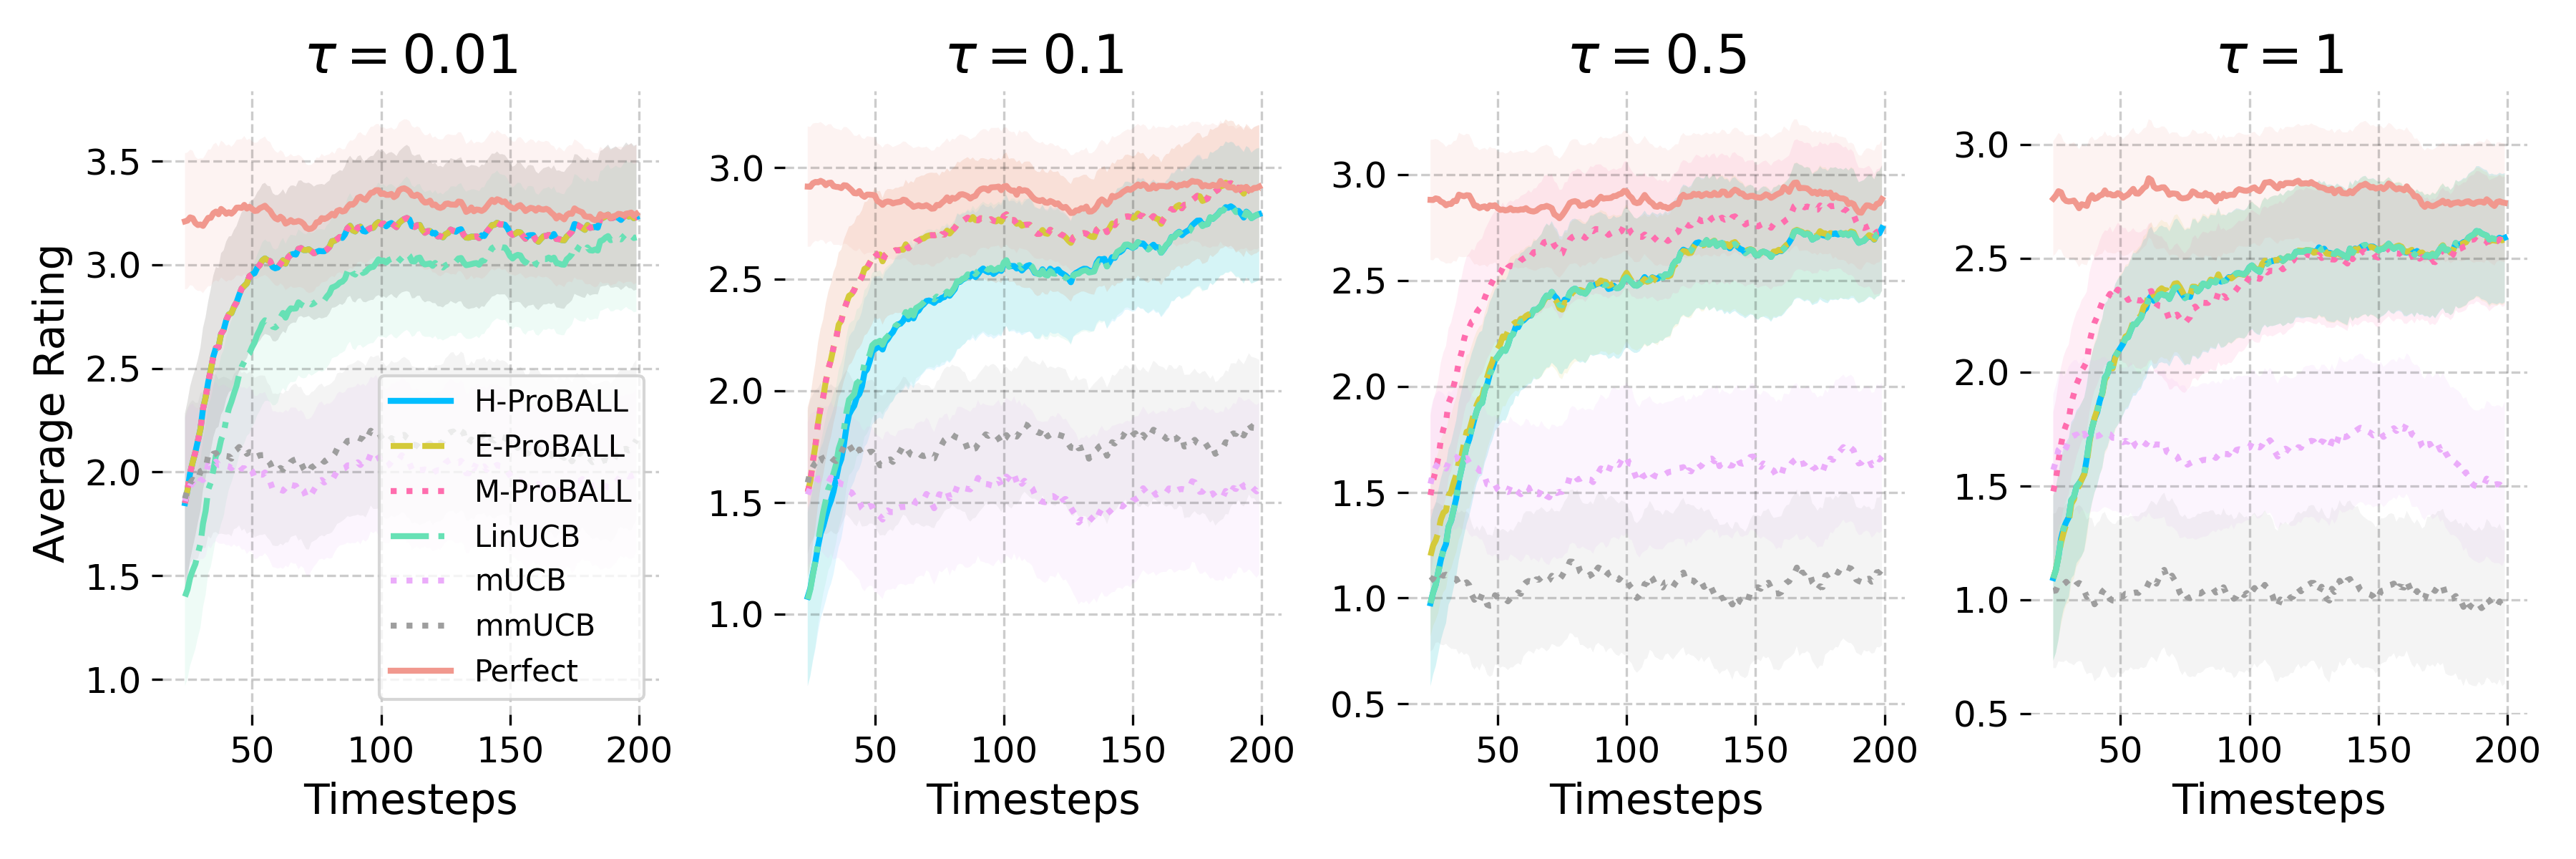
\includegraphics[scale=0.55]{figures/ch03/imgs/movies/bayes_rating_movies.png}
    \caption{Comparison of \aigen{Algorithm~\ref{alg:proball-ucb}} initialized with ground truth subspaces against LinUCB, mUCB, and mmUCB, for different choices of $\tau$ and confidence bound constructions, in terms of rolling average rating over $25$ timesteps. All variants of \aigen{Algorithm~\ref{alg:proball-ucb}} perform no worse than LinUCB, and outperform mUCB and mmUCB. Shaded area depicts $1$-standard error confidence intervals over 30 trials with fresh $\theta$. The confidence intervals on regret thus account for the variation in frequentist regret for changing $\theta$.}
    \label{fig:movie-rating-no-sold-ts}
\end{figure}
 
\end{minipage}

\newpage
\subsection{Sample Complexity of \aigen{Algorithm~\ref{alg:sold}}}

We perform an empirical study of the sample complexity of \aigen{Algorithm~\ref{alg:sold}} on the MovieLens dataset. To do so, we compare the end-to-end regret at $T=200$ timesteps of both \aigen{Algorithm~\ref{alg:proball-ucb}} and \aigen{projected confidence-ball Thompson sampling (Algorithm~\ref{alg:proball-ts})}, against LinUCB and Linear Thompson sampling using ground-truth low-dimensional features. When $\tau$ is small enough, we see that the end-to-end regret of both \aigen{Algorithm~\ref{alg:proball-ucb}} and \aigen{projected confidence-ball Thompson sampling (Algorithm~\ref{alg:proball-ts})} converges to that of LinUCB and Linear Thompson sampling using ground-truth low-dimensional features. This shows that we lose little from needing to estimate the subspace with \aigen{Algorithm~\ref{alg:sold}} when enough offline samples are present.


\begin{figure}[H]
    \centering
    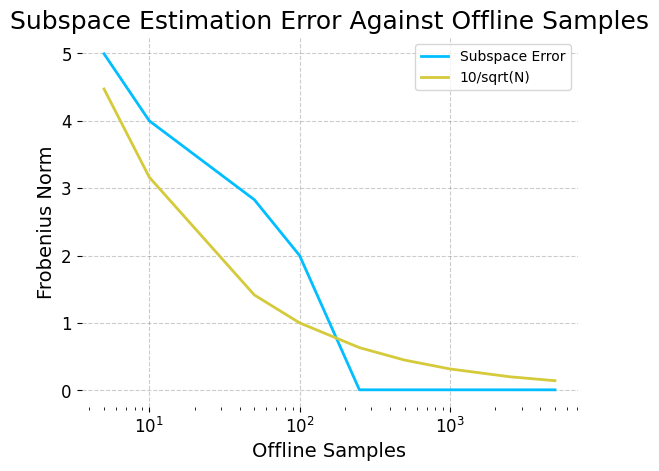
\includegraphics[width=0.7\linewidth]{figures/ch03/imgs/movies/sample_comp_sold.png}
    \caption{Subspace estimation error of \aigen{Algorithm~\ref{alg:sold}} against the number of offline samples, in the Frobenius norm. This was performed on the MovieLens dataset. We compare the error of \aigen{Algorithm~\ref{alg:sold}} against the parametric rate of $1/\sqrt{N}$. This shows that the error of \aigen{Algorithm~\ref{alg:sold}} indeed decreases very quickly in practice.}
    \label{fig:subspace-error-sold}
\end{figure}

\newpage
\begin{figure}[H]
    \centering
    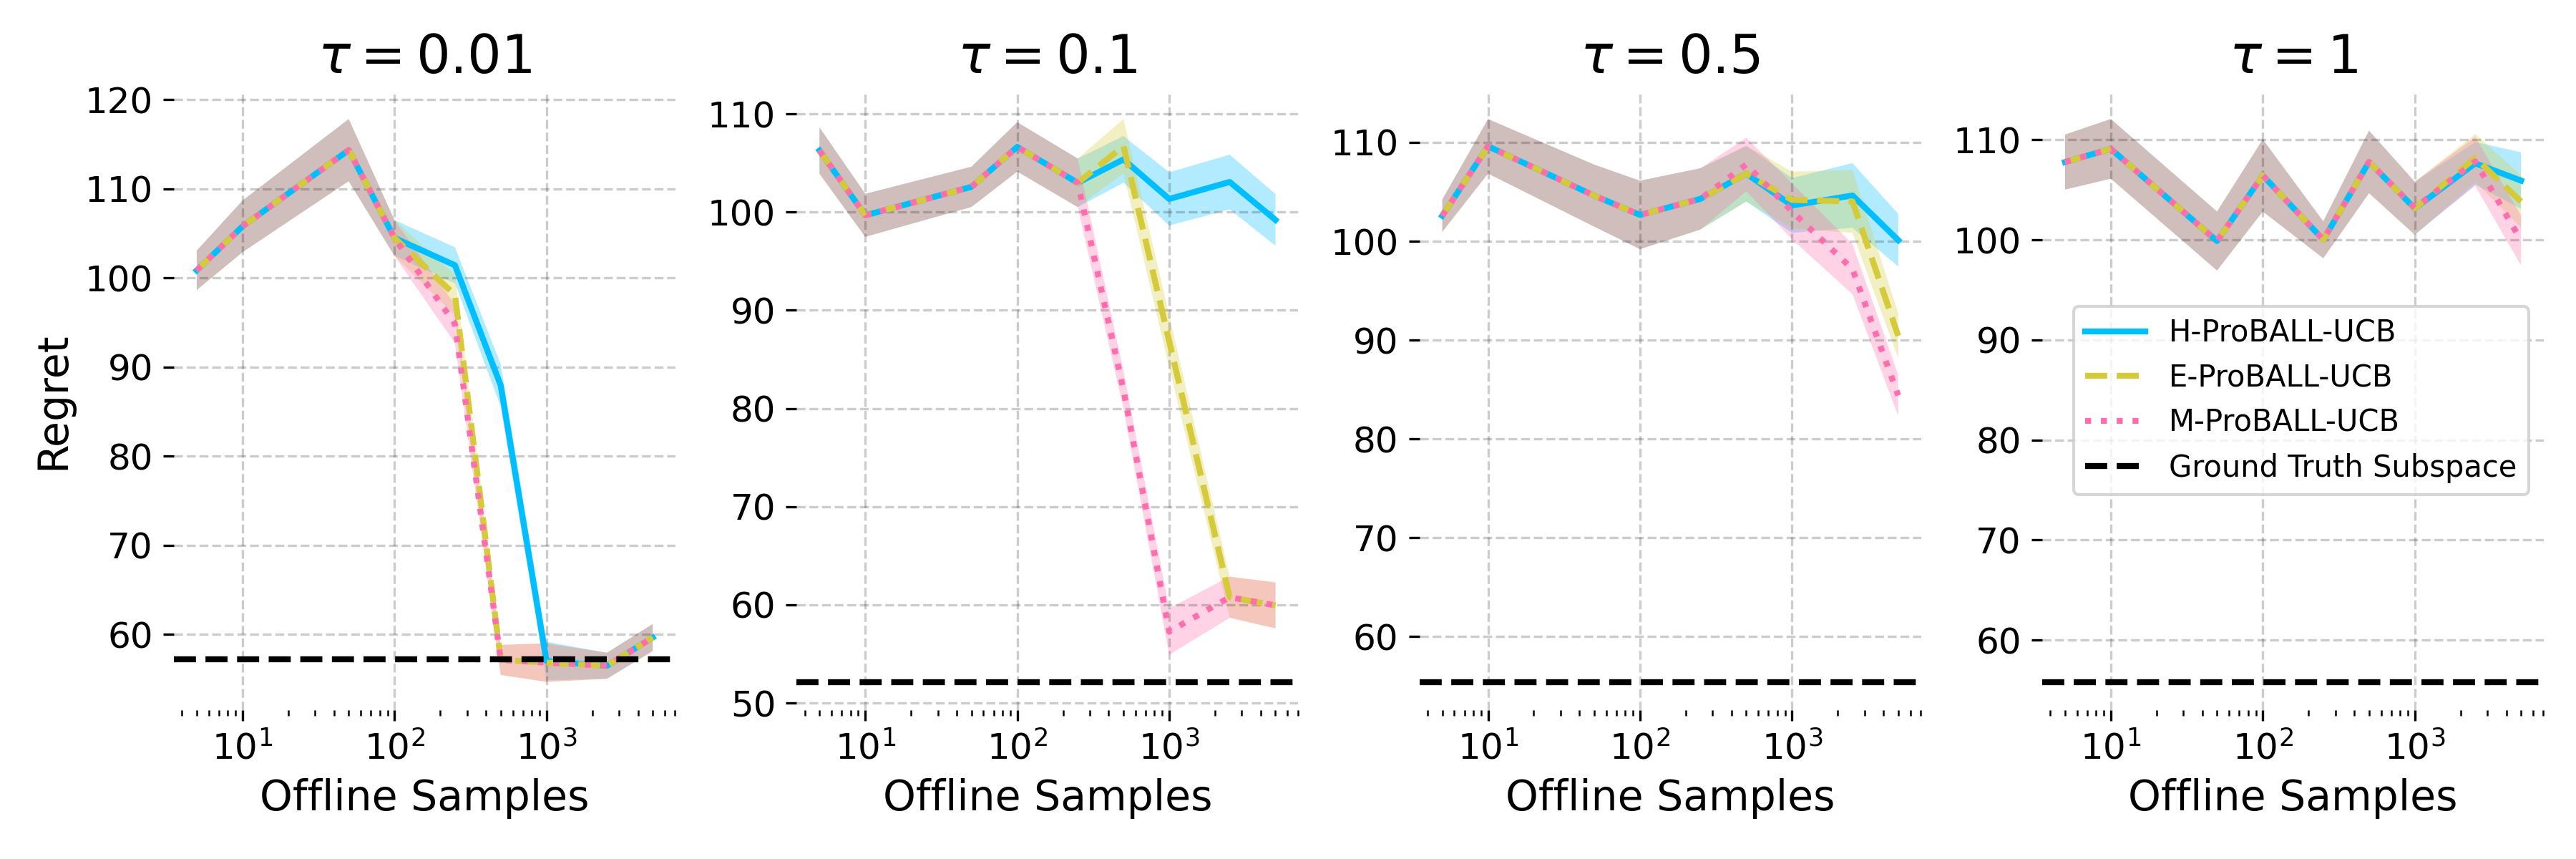
\includegraphics[scale=0.55]{figures/ch03/imgs/movies/bayes_subspace_sample_comp_movies.png}
    \caption{End-to-end regret at $T=200$ timesteps of \aigen{Algorithm~\ref{alg:proball-ucb}} initialized with \aigen{Algorithm~\ref{alg:sold}}, against the number of offline samples used in fitting \aigen{Algorithm~\ref{alg:sold}}. With a low enough $\tau$, the regret of \aigen{Algorithm~\ref{alg:proball-ucb}} approaches the regret of LinUCB on ground-truth low-dimensional features, showing that we lose next to nothing from needing to estimate the subspace with \aigen{Algorithm~\ref{alg:sold}}. Shaded area depicts $1$-standard error confidence intervals over 30 trials with fresh $\theta$. }
    \label{fig:sample-complexity-sold-ucbs}
\end{figure}


\begin{figure}[H]
    \centering
    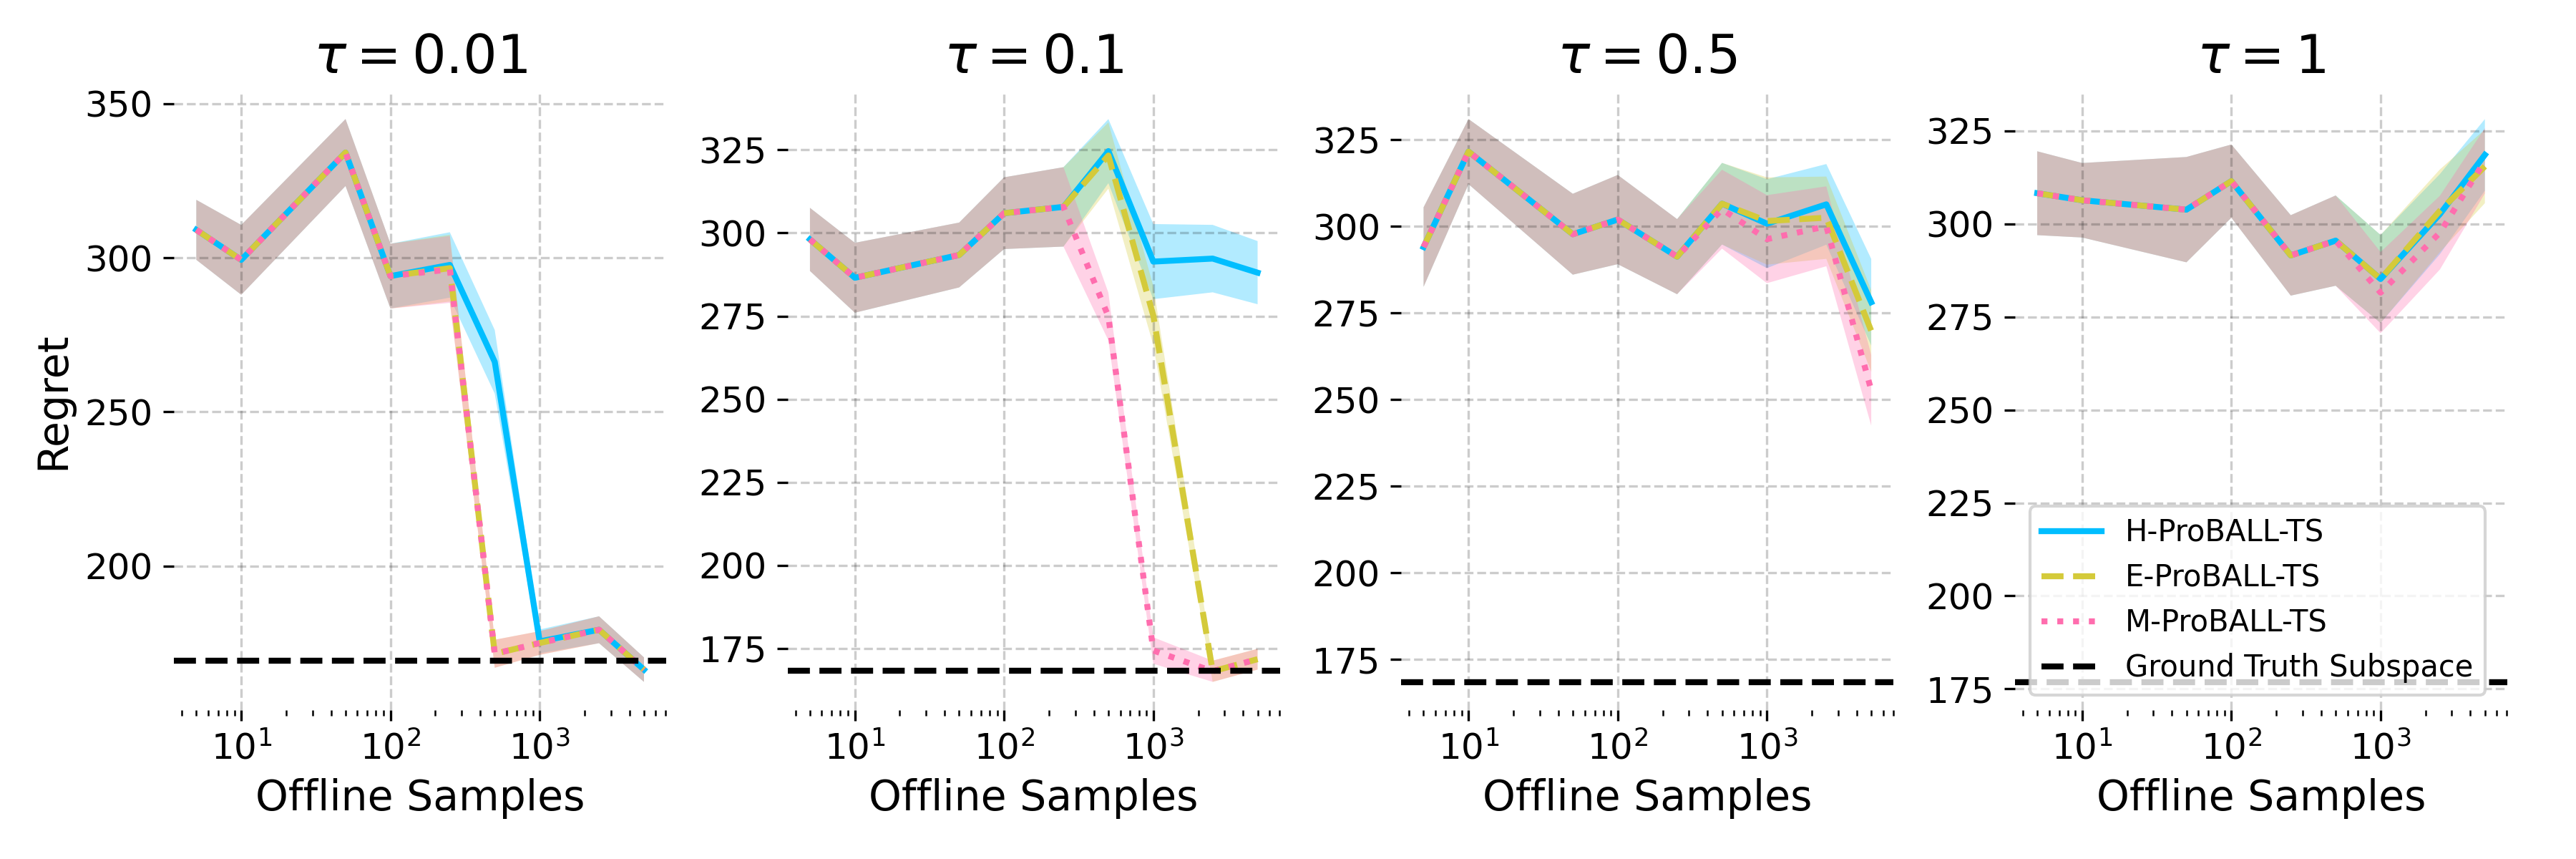
\includegraphics[scale=0.55]{figures/ch03/imgs/movies/bayes_subspace_ts_sample_comp_movies.png}
    \caption{End-to-end regret at $T=200$ timesteps of \aigen{projected confidence-ball Thompson sampling (Algorithm~\ref{alg:proball-ts})} initialized with \aigen{Algorithm~\ref{alg:sold}}, against the number of offline samples used in fitting \aigen{Algorithm~\ref{alg:sold}}. With a low enough $\tau$, the regret of \aigen{projected confidence-ball Thompson sampling (Algorithm~\ref{alg:proball-ts})} approaches the regret of TS on ground-truth low-dimensional features, showing that we lose next to nothing from needing to estimate the subspace with \aigen{Algorithm~\ref{alg:sold}}. Shaded area depicts $1$-standard error confidence intervals over 30 trials with fresh $\theta$. }
    \label{fig:sample-complexity-sold-ts}
\end{figure}
